%\documentclass[11pt]{article}
\documentclass[final,12pt]{colt2018}

\usepackage[T1]{fontenc}

%\usepackage{geometry}
% \usepackage[letterpaper, left=1in, right=1in, top=1in, bottom=1in]{geometry}

%\usepackage[dvipsnames]{xcolor}
%\usepackage[colorlinks=true, linkcolor=blue, citecolor=blue]{hyperref}
\usepackage{microtype} 

\usepackage{algorithm}
\usepackage{algpseudocode}

%\usepackage{parskip}

% \usepackage{natbib}
% \bibliographystyle{plainnat}
% \bibpunct{(}{)}{;}{a}{,}{,}

% \usepackage{amsthm}
\usepackage{mathtools}
\usepackage{amsmath}
\usepackage{bbm}
\usepackage{amsfonts}
\usepackage{amssymb}
\let\vec\undefined
\usepackage{MnSymbol} %Actually conflicts with amssymb and others

\usepackage{xpatch}

%%% theorems

% \theoremstyle{definition}  %Sets style of subsequent newtheorems to 'definition'
% \newtheorem{exercise}{Exercise}
% \newtheorem{claim}{Claim}
% \newtheorem{lemma}{Lemma}
\newtheorem{assumption}{Assumption}
% \newtheorem{conjecture}{Conjecture}
% \newtheorem{corollary}{Corollary}
% \newtheorem{proposition}{Proposition}
\newtheorem{fact}{Fact}
% %\newtheorem{model}{Model}
% %\newtheorem{problem}{Problem}
% \newtheorem{assumption}{Assumption}
% \newtheorem{problem}{Problem}
% \newtheorem{model}{Model}
% \theoremstyle{plain}
% \newtheorem{remark}{Remark}
% \newtheorem{example}{Example}
% \newtheorem{theorem}{Theorem}
% \newtheorem{definition}{Definition}

\xpatchcmd{\proof}{\itshape}{\normalfont\proofnameformat}{}{}
\newcommand{\proofnameformat}{\bfseries}

\newcommand{\notimplies}{\nRightarrow}

%%% prettyref

\usepackage{prettyref}
\newcommand{\pref}[1]{\prettyref{#1}}
% \newcommand{\pfref}[1]{Proof of \prettyref{#1}}
\newcommand{\pfref}[1]{{\bf of \prettyref{#1}}}
\newcommand{\savehyperref}[2]{\texorpdfstring{\hyperref[#1]{#2}}{#2}}
\newrefformat{eq}{\savehyperref{#1}{\textup{(\ref*{#1})}}}
\newrefformat{eqn}{\savehyperref{#1}{Equation~\ref*{#1}}}
\newrefformat{lem}{\savehyperref{#1}{Lemma~\ref*{#1}}}
\newrefformat{fact}{\savehyperref{#1}{Fact~\ref*{#1}}}
\newrefformat{def}{\savehyperref{#1}{Definition~\ref*{#1}}}
\newrefformat{thm}{\savehyperref{#1}{Theorem~\ref*{#1}}}
\newrefformat{corr}{\savehyperref{#1}{Corollary~\ref*{#1}}}
\newrefformat{sec}{\savehyperref{#1}{Section~\ref*{#1}}}
\newrefformat{app}{\savehyperref{#1}{Appendix~\ref*{#1}}}
\newrefformat{ass}{\savehyperref{#1}{Assumption~\ref*{#1}}}
\newrefformat{ex}{\savehyperref{#1}{Example~\ref*{#1}}}
\newrefformat{fig}{\savehyperref{#1}{Figure~\ref*{#1}}}
\newrefformat{alg}{\savehyperref{#1}{Algorithm~\ref*{#1}}}
\newrefformat{rem}{\savehyperref{#1}{Remark~\ref*{#1}}}
\newrefformat{conj}{\savehyperref{#1}{Conjecture~\ref*{#1}}}
\newrefformat{prop}{\savehyperref{#1}{Proposition~\ref*{#1}}}
\newrefformat{proto}{\savehyperref{#1}{Protocol~\ref*{#1}}}
\newrefformat{prob}{\savehyperref{#1}{Problem~\ref*{#1}}}
\newrefformat{claim}{\savehyperref{#1}{Claim~\ref*{#1}}}

% Math delimiters
\DeclarePairedDelimiter{\abs}{\lvert}{\rvert} %
\DeclarePairedDelimiter{\brk}{[}{]}
\DeclarePairedDelimiter{\crl}{\{}{\}}
\DeclarePairedDelimiter{\prn}{(}{)}
\DeclarePairedDelimiter{\nrm}{\|}{\|}
\DeclarePairedDelimiter{\tri}{\langle}{\rangle}
\DeclarePairedDelimiter{\dtri}{\llangle}{\rrangle}

\DeclarePairedDelimiter{\ceil}{\lceil}{\rceil}
\DeclarePairedDelimiter{\floor}{\lfloor}{\rfloor}


% \DeclareMathOperator{\E}{\mathbb{E}} %expecation
\let\Pr\undefined
\let\P\undefined
\DeclareMathOperator*{\En}{\mathbb{E}}
\DeclareMathOperator{\Enn}{\mathbb{E}}
\DeclareMathOperator*{\Eh}{\widehat{\mathbb{E}}}
\DeclareMathOperator{\P}{P}
\DeclareMathOperator{\Pr}{Pr}

% Arg<x>
\DeclareMathOperator*{\argmin}{arg\,min} % * Places subscript directly under operator
\DeclareMathOperator*{\argmax}{arg\,max}             
\DeclareMathOperator*{\arginf}{arg\,inf} 
\DeclareMathOperator*{\argsup}{arg\,sup} 

\DeclareMathOperator*{\smax}{smax_{\eta}}
\DeclareMathOperator*{\smin}{smin_{\eta}}

% one-off macros
\newcommand{\ls}{\ell}
\newcommand{\ind}{\mathbbm{1}}    %Indicator
\newcommand{\pmo}{\crl*{\pm{}1}}
\newcommand{\eps}{\epsilon}
\newcommand{\veps}{\varepsilon}

\newcommand{\ldef}{\vcentcolon=}
\newcommand{\rdef}{=\vcentcolon}

% styles
\newcommand{\mc}[1]{\mathcal{#1}}
\newcommand{\wt}[1]{\widetilde{#1}}
\newcommand{\wh}[1]{\widehat{#1}}


% Special letters: blackboard, mathcal, widehat
% djhsu magic
\def\ddefloop#1{\ifx\ddefloop#1\else\ddef{#1}\expandafter\ddefloop\fi}
\def\ddef#1{\expandafter\def\csname bb#1\endcsname{\ensuremath{\mathbb{#1}}}}
\ddefloop ABCDEFGHIJKLMNOPQRSTUVWXYZ\ddefloop
\def\ddefloop#1{\ifx\ddefloop#1\else\ddef{#1}\expandafter\ddefloop\fi}
\def\ddef#1{\expandafter\def\csname b#1\endcsname{\ensuremath{\mathbf{#1}}}}
\ddefloop ABCDEFGHIJKLMNOPQRSTUVWXYZ\ddefloop
\def\ddef#1{\expandafter\def\csname c#1\endcsname{\ensuremath{\mathcal{#1}}}}
\ddefloop ABCDEFGHIJKLMNOPQRSTUVWXYZ\ddefloop
\def\ddef#1{\expandafter\def\csname h#1\endcsname{\ensuremath{\widehat{#1}}}}
\ddefloop ABCDEFGHIJKLMNOPQRSTUVWXYZ\ddefloop
\def\ddef#1{\expandafter\def\csname hc#1\endcsname{\ensuremath{\widehat{\mathcal{#1}}}}}
\ddefloop ABCDEFGHIJKLMNOPQRSTUVWXYZ\ddefloop
\def\ddef#1{\expandafter\def\csname t#1\endcsname{\ensuremath{\widetilde{#1}}}}
\ddefloop ABCDEFGHIJKLMNOPQRSTUVWXYZ\ddefloop
\def\ddef#1{\expandafter\def\csname tc#1\endcsname{\ensuremath{\widetilde{\mathcal{#1}}}}}
\ddefloop ABCDEFGHIJKLMNOPQRSTUVWXYZ\ddefloop

% Names
\newcommand{\Holder}{H{\"o}lder}
% Custom commands
\newcommand{\bR}{\mathbb{R}}
\newcommand{\mL}{\mathcal{L}}
\newcommand{\mO}{\mathcal{O}}
\newcommand{\mG}{\mathcal{G}}
\newcommand{\mF}{\mathcal{F}}
\newcommand{\mP}{\mathcal{P}}
\newcommand{\mR}{\mathcal{R}}
\newcommand{\bI}{\mathbf{1}}
\newcommand{\TV}{d_{\text{TV}}}
\newcommand{\KL}{d_{\text{KL}}}
\newcommand{\Tr}{\text{Tr}}
\newcommand{\bP}{\mathbb{P}}
\newcommand{\bE}{\mathbb{E}}

\newcommand{\N}{\mathcal{N}}
\newcommand{\Id}{\mathsf{I}}
\newcommand{\las}{\mathsf{las}}
\newcommand{\spca}{\mathsf{spca}}

\newcommand{\Yt}{\widetilde{Y}}
\newcommand{\Wt}{\widetilde{W}}


% Standard environments
%\newtheorem{definition}{Definition}[section]
%\newtheorem{example}{Example}[section]
%\newtheorem{exercise}{Exercise}[section]
\newtheorem{fact}{Fact}[section]
%\newtheorem{theorem}{Theorem}[section]
%\newtheorem{corollary}{Corollary}[section]
%\newtheorem{conjecture}{Conjecture}[section]
%\newtheorem{lemma}{Lemma}[section]
%\newtheorem{problem}{Problem}[section]
\newenvironment{solution}[1][Solution]{
    \begin{proof}[#1]
  }{
    \end{proof}
  }

\newenvironment{fminipage}%
  {\begin{Sbox}\begin{minipage}}%
  {\end{minipage}\end{Sbox}\fbox{\TheSbox}}

\newenvironment{algbox}[0]{\vskip 0.2in
\noindent 
 \begin{fminipage}{5.9in}
}{
\end{fminipage}
\vskip 0.2in
}

\setcounter{tocdepth}{1}

%\usepackage[suppress]{color-edits}
%\usepackage{color-edits}
%\addauthor{df}{red}
%\addauthor{ks}{blue}
%\usepackage{showlabels}

%%%% Misc macros

% \newcommand{\pt}{\partial_{t}}
%\newcommand{\dl}{\partial}
\newcommand{\reg}{\mathrm{Reg}_n}
\renewcommand{\trn}{\top}
\newcommand{\dl}{\delta}
\newcommand{\sym}{\mathbb{S}}
\newcommand{\Bfun}{Burkholder }

\newcommand{\predt}{\wt{y}}

\newcommand{\propone}{$1^{o}$}
\newcommand{\proptwo}{$2^{o}$}
\newcommand{\propthree}{$3^{o}$}
\newcommand{\propthreep}{$3'$}

%%%% document info %%%%%%%

\title[Online Learning: Sufficient Statistics and the Burkholder Method]{Online Learning: Sufficient Statistics and the Burkholder Method}
\usepackage{times}

\date{}

%\author{
%  Dylan J. Foster\thanks{Cornell University}
%  \and
%  Alexander Rakhlin\thanks{MIT}
%  \and
%  Karthik Sridharan\footnotemark[1]
%  }
  \coltauthor{\Name{Dylan J. Foster}\Email{djfoster@cs.cornell.edu}\\
\addr Cornell University
\AND
\Name{Alexander Rakhlin}\Email{rakhlin@mit.edu}\\
\addr Massachusetts Institute of Technology
\AND
\Name{Karthik Sridharan}\Email{sridharan@cs.cornell.edu}\\
\addr Cornell University
  }

\begin{document}

\maketitle

\begin{abstract}
We uncover a fairly general principle in online learning: If a regret inequality can be (approximately) expressed as a function of certain ``sufficient statistics'' for the data sequence, then there exists a special \emph{Burkholder function} that 1) can be used algorithmically to achieve the regret bound and 2) only depends on these sufficient statistics, not the entire data sequence,  so that the online strategy is only required to keep the sufficient statistics in memory. This characterization is achieved by bringing the full power of the \emph{Burkholder Method}---originally developed for certifying probabilistic martingale inequalities---to bear on the online learning setting.

To demonstrate the scope and effectiveness of the Burkholder method, we develop a novel online strategy for matrix prediction that attains a regret bound corresponding to the variance term in matrix concentration inequalities. We also present a linear-time/space prediction strategy for parameter-free supervised learning with linear classes and general smooth norms. 

\end{abstract}

\section{Introduction}
% !TeX root = main.tex
\section{Introduction}
\label{sec:intro}
Generative models are often trained in an unsupervised fashion, fitting a model $q$ to a set of observed data $x_P \subseteq X$ drawn iid from some true distribution $p$ on $x\in X$. Now, of course $p$ may not exactly belong to family $Q$ of probability distributions being fit, whether $Q$ consists of Gaussians mixture models, Markov models, or even neural networks of bounded size. We first discuss the limitations of generative modeling without feedback, and then discuss our model and results.

%\subsection{Limitations of Generative Modeling from Positive Examples Alone}
Consider fitting a generative model on a text corpus consisting partly of poetry written by four-year-olds and partly of mathematical publications from the {\em Annals of Mathematics}. Suppose that learning to generate a poem that looks like it was written by a child was easier than learning to generate a novel mathematical article with a correct, nontrivial statement. If the generative model pays a high price for generating unrealistic examples, then it may be better off learning to generate children's poetry than mathematical publications. However, without negative feedback, it may be difficult for a neural network or any other model to know that the mathematical articles it is generating are stylistically similar to the mathematical publications but do not contain valid proofs.\footnote{This is excluding clearly fake articles published without proper review in lower-tier venues \citep{LabbeL13}.} 

As a simpler example, the classic Markovian ``trigram model'' of natural language assigns each word a fixed probability conditioned only on the previous two words. Prior to recent advances in deep learning, for decades the trigram model and its variant were the workhorses of language modeling, assigning much greater likelihood to natural language corpora than numerous linguistically motivated grammars and other attempts \citep{Rosenfeld00}. However, text sampled from a trigram is typically nonsensical, e.g., the following text was randomly generated from a trigram model fit on a corpus of text from the Wall Street Journal \citep{JurafskyM09}:
\begin{quote}
They also point to ninety nine point six billion dollars from two hundred
four oh six three percent of the rates of interest stores as Mexico and
gram Brazil on market conditions. 
\end{quote}

In some applications, like text compression using a language model \citep{WittenNC87}, maximizing likelihood is equivalent to optimizing compression. However, in many  applications involving generation, such nonsense is costly and unacceptable. Now, of course it is possible to always generate valid data by returning random training examples, but this is simply overfitting and not learning. Alternatively, one could incorporate human-in-the-loop feedback such as through crowdsourcing, into the generative model to determine what is a valid, plausible sentence.

In some domains, validity could be determined automatically. Consider a Markovian model of a well-defined concept such as mathematical formulas that compile in \LaTeX{}. Now, consider a $n$-gram Markovian character model which the probability of each subsequent character is determined by the previous $n$ characters. For instance, the expression \$\{2+\{x-y\}\$ is invalid in \LaTeX{} due to mismatched braces. For this problem, a \LaTeX{} compiler may serve as a validity oracle. Various $n$-gram models can be fit which only generate valid formulas. To address mismatched braces, for example, one such model would ensure that it always closed braces within $n$ characters of opening, and had no nested braces. While an $n$-gram model will not perfectly model the true distribution over valid \LaTeX{} formulas, for certain generative purposes one may prefer an $n$-gram model that generates valid formulas over one that assigns greater likelihood to the training data but generates invalid formulas. 

Figure \ref{fig:rectangle} illustrates a simple case of learning a rectangle model for data which is not uniform over a rectangle. A maximum likelihood model would necessarily be the smallest rectangle containing all the data, but most examples generated from this distribution may be invalid. Instead a smaller rectangle, as illustrated in the figure, may be desired.

\begin{figure}[h]\label{fig:rectangle}
\centering
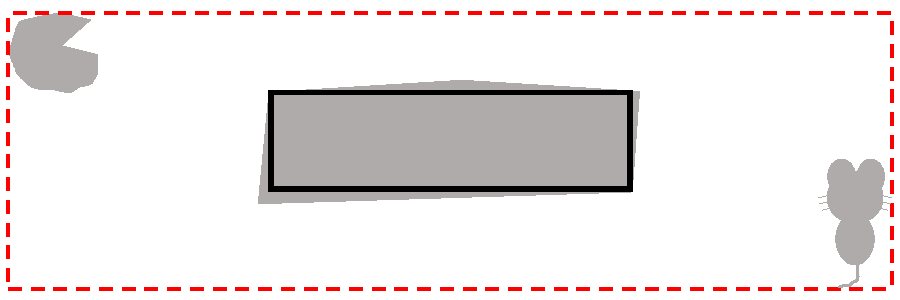
\includegraphics[width=3in]{fig.pdf}
\caption{Example where the underlying distribution $p$ is uniform over the (gray) valid regions. The solid rectangle maximizes our objective since it does not output nonsense (is supported only within the grey matter) and is closest to the $p$ (covers the maximum amount of grey matter). In contrast, the standard maximum likelihood (dashed red) rectangle must fully contain the observed samples, thus generating invalid points most of the time.  }
\end{figure}

Motivated by these observations, we evaluate a generative model $q$ on two axes. First is {\em coverage}, which is related to the probability assigned to future examples drawn from the true distribution $p$. Second is {\em validity}, defined as the probability that random examples generated from $q$ meet some validity requirement. Formally, we measure coverage in terms of a bounded {\em loss}:
$$\Loss(p,q)=\E_{x \sim p}[L(q_x)],$$
where $L:[0,1]\rightarrow [0,M]$ is a bounded decreasing function such as the capped log-loss $L(q_x)=\min(M, \log 1/q_x)$. % or $L(q_x)=\log 1/(q_x+\exp(-M))$. 
A bounded loss has the advantages of being efficiently estimable, and also it enables a model to assign 0 probability to one example (e.g., an outlier or error) if it greatly increases the likelihood of all other data. Validity is defined with respect to a set $V \subseteq X$, and $q(V)$ is the probability that a random example generated from $q$ lies within $V$. 

Clearly, there is a tradeoff between coverage and validity. We first focus on the case of (near) perfect validity. A Valid Generative Modeling (VGM) algorithm if it outputs, for a family of distributions $Q$ over $X$, if it outputs $\hat{q}$ with (nearly) perfect validity and whose loss is nearly as good as the loss of the best valid $q\in Q$. More precisely, $A$ is a VGM learner of $Q$ if for any nonempty valid subset $V \subseteq X$, any probability distribution $p$ over $V$, and any $\eps>0$, $A$ uses $n$ random samples from $p$ and makes $m$ membership oracle calls to $V$ and outputs a distribution $\hat{q}$ such that, $$\Loss(p, \hat{q}) \leq \min_{q \in Q: q(V)=1}\Loss(p,q) + \eps ~\text{ and }~\hat{q}(V)\geq 1-\eps.$$ 
We aim for our learner to be sample and query efficient, requiring that $n$ and $m$ are polynomial in $M, 1/\eps$ and a measure of complexity of our distribution class $Q$.
Furthermore, we would like our algorithms to be computationally efficient, with a runtime polynomial in the size of the data, namely the $n + m$ training examples. 
A more formal description of the problem is available in Section~\ref{sec:problem}.

$A$ is said to be {\em proper} if it always outputs $\hat{q}\in Q$ and {\em improper} otherwise.
In Section~\ref{sec:impossibility}, we first show that efficient proper learning for VGM is impossible. This is an information-theoretic result, meaning that even given infinite runtime and positive samples, one still cannot solve the VGM problem. Interestingly, this is different from binary classification, where it is possible to statistically learn from iid examples without a membership oracle.

Our first main positive result is an efficient (improper) learner for VGM. The algorithm relies on a subroutine that solves the following {\em Generative Modeling with Negatives} (GMN) problem: given sets $X_P, X_N \subset X$ of positive and negative examples, find the probability distribution $q \in Q$ which minimizes $\sum_{x \in X_P} L(q(x))$ subject to the constraint that $q(X_N)=0$. For simplicity, we present our algorithm for the case that the distribution family $Q$ is finite, giving sample and query complexity bounds that are logarithmic in terms of $|Q|$. However, as we show in Section~\ref{sec:infinite-families}, all of our results extend to infinite families $Q$. It follows that if one has a computationally efficient algorithm for the GMN problem for a distribution family $Q$, then our reduction gives a computationally efficient VGM learning algorithm for $Q$.

Our second positive result is an algorithm that minimizes $\Loss(p,q)$ subject to a relaxed validity constraint comparing against the optimal distribution that has validity $q(V)$ at least $1-\alpha$ for some $\alpha>0$. We show in Section~\ref{sec:partial-validity} that even in this more general setting, it is possible to obtain an algorithm that is statistically efficient but may not be computationally efficient. An important open question is whether there exists a computationally efficient algorithm for this problem when given access to an optimization oracle, as was the case for our algorithm for VGM.

\subsection{Related Work}
\cite{KearnsMRRSS94} showed how to learn distributions from positive examples in the realizable setting, i.e., where the true distribution is assumed to belong to the class being learned. In the same sense as their work is similar to PAC learning \citet{Valiant84} of distributions, our work is like agnostic learning \citet{KearnsSS94} in which no assumption on the true distribution is made. 

Generative Adversarial Networks (GANs)~\cite{GoodfellowPMXWOCB14} are an approach for generative modeling from positive examples alone, in which a generative model is trained against a discriminator that aims to distinguish real data from generated data. In some domains, GANs have been shown to outperform other methods at generating realistic-looking examples. Several shortcomings of GANs have been observed \citet{AroraRZ18}, and GANs are still subject to the theoretical limitations we argue are inherent to any model trained without a validity oracle. 

In supervised learning, there is a rich history of learning theory with various types of queries, including membership which are not unlike our (in)validity oracle. Under various assumptions, queries have been shown to facilitate the learning of complex classes such as finite automata \citet{Angluin88} and DNFs \citet{Jackson97}. See the survey of \cite{Angluin92} for further details.  Interestingly, \cite{Feldman09} has shown that for agnostic learning, i.e., without making assumptions on the generating distribution, the addition of membership queries does not enhance what is learnable beyond random examples alone. 
Supervised learning also has a large literature around active learning, showing how the ability to query examples reduces the sample complexity of many algorithms. See the survey of \cite{Hanneke14}. Note that the aim here is typically to save examples and not to expand what is learnable.
 
More sophisticated models, e.g., involving neural networks, can mitigate the invalidity problem as they often generate more realistic natural language and have even been demonstrated to generate \LaTeX{} that nearly compiles \citep{Karpathy15} or nearly valid Wikipedia markdown. However, longer strings generated are unlikely to be valid. For example, \cite{Karpathy15} shows generated markdown which includes:
\begin{quote}
==Access to ''rap===
The current history of the BGA has been [[Vatican Oriolean Diet]], British Armenian, published in 1893.  While actualistic such conditions such as the [[Style Mark Romanians]] are still nearly not the loss.
\end{quote}

Even ignoring the mismatched quotes and equal signs, note that this example has two so-called ``red links'' to two pages that do not exist. Without checking, it was not obvious to us whether or not Wikipedia had pages titled {\em Vatican Oriolean Diet} or {\em Style Mark Romanians}. In some applications, one may or may not want to disallow red links. In the case that they are considered valid, one may seek a full generative model of what might plausibly occur inside of brackets, as the neural network has learned in this case. If they are disallowed, a model might memorize links it has seen but not generate new ones. A validity oracle can help the learner identify what it should avoid generating.

 In practice, \cite{KusnerPH17} discuss how generative models from neural networks (in particular autoencoders) often generate invalid sequences. 
\cite{JanzWPKH18} learn the validity of examples output by a generative model using oracle feedback. 




\section{Example: Matrix Prediction}
\label{sec:matrix}
% !TEX root = paper.tex

In this section we focus on linear matrix prediction problems. The side information $x_t$ is now matrix-valued, and we shall denote it by a capital letter $X_t\in\bbR^{d_1\times{}d_2}$. Our goal is to achieve a regret inequality as in \pref{eq:phi_comp_adap} with a class $\F=\crl*{X\mapsto\tri*{W,X}\mid{} W\in\cW}$, where $\cW=\crl*{W\in\bbR^{d_1\times{}d_2}\mid{}\nrm*{W}_{\Sigma}\leq{}r}$. Here $\tri*{A,B}=\Tr(AB^{\trn})$ is the standard matrix inner product and $\nrm*{\cdot}_{\Sigma}$ denotes the nuclear norm. We also let $\nrm*{\cdot}_{\sigma}$ denote the spectral norm. As before, the loss $\loss$ is assumed to be $L$-Lipschitz and regret against a matrix $W\in\cW$ is given by
$
  \reg(W)\ldef \sum_{t=1}^{n}\loss(\pred_t, y_t) - \loss(\tri*{W,X_t}, y_t).
$

In a search for an adaptive bound on regret, we inspect the adaptive bound \pref{eq:adaptive} for the vector case. The direct analogue for matrices would be a bound proportional to $\left(\sum_{t=1}^n \norm{X_t}^2_\sigma \right)^{1/2}$, and indeed such a bound is possible with Matrix Exponential Weights \cite[Theorem 13]{HazKalSha12}.\footnote{With more work it is possible to obtain a bound of $\left(\max_{t}\nrm*{X_t}_{\sigma}\cdot\nrm*{\sum_{t=1}^nX_t}_\sigma \right)^{1/2}$; this is still weaker than our result, and seems to only be possible when the constraint set and $X_t$s are restricted to be positive-semidefinite.} However, the matrix version of Khintchine inequality, as well as matrix deviation inequalities, involve---for the case of random centered self-adjoint matrices---the tighter quantity $\norm{\sum_{t=1}^n X_t^2}^{1/2}_\sigma$ (see \citep{tropp2012user,mackey2014matrix}). Given the correspondence between online regret bounds and martingale inequalities, one may wonder if there is an algorithm that achieves this adaptive bound. We shall exhibit such a method using our approach, and the reader might already guess that $\sum_{t=1}^n X_t^2$ should be part of the sufficient statistic for the online algorithm. This is indeed the case, though we present results for general non-square matrices.

Let $\sym^{d}$ denote the set of symmetric matrices in $\bbR^{d\times{}d}$, $\sym^{d}_{+}$ denote the set of positive-semidefinite matrices, and $\sym^{d}_{++}$ denote the set of positive-definite matrices. 
For $X\in\sym^{d}$ we let $\lambda(X)\in\bbR^{d}$ denote its eigenvalues arranged in decreasing order, so that $\lambda_1(X)$ is the largest eigenvalue. For any matrix $X\in\bbR^{d_1\times{}d_2}$ we define its Hermitian dilation $\cH(X)\in\sym^{d_1+d_2}$ and  $\cM(X) \in\sym^{d_1+d_2}$ as:
\begin{equation}
  \cH(X) = \left(
    \begin{array}{ll}
      0 & X\\
      X^{\trn} & 0
    \end{array}
    \right) ~~~~~~~~~\cM(X) = \cH(X)^{2} = \left(
    \begin{array}{ll}
      XX^{\trn} & 0\\
      0 & X^{\trn}X
    \end{array}
  \right).
  \end{equation}
  It is well-known that for any matrix $X$, $\lambda_{1}(\cH(X)) = \nrm*{X}_{\sigma}.$

With these definitions in place, the desired adaptive regret bound takes the form
\begin{equation}
\cA_{\eta}(X_{1},\ldots,X_{n}) = \frac{\eta{}rL^2}{2}\nrm*{\sum_{t=1}^{n}\cM(X_t)}_{\sigma} + \frac{c}{\eta}
\end{equation}
for some fixed $\eta>0$ and constant $c>0$. The sufficient statistic takes values in  $\cT=\reals\times \sym^{d_1+d_2}\times \sym^{d_1+d_2}_{+}$ and incorporates the matrix variance terms $\cM(X_t)$.



\begin{proposition}
  \label{prop:matrix_sufficient}
  The pair $(\suff, V)$ defined via $\suff(X_t,\pred_t,\delta_t) = \left( \delta_t\cdot\pred_t, \delta_t\cdot \cH(X_t), \cM(X_t) \right)\in\reals\times \sym^{d_1+d_2}\times \sym^{d_1+d_2}_{+}$ and
\begin{equation}
\label{eq:matrix_v}
V(a, H, M) = a + r\lambda_1\prn*{H -{\textstyle\frac{1}{2}}\eta{}L^2 M} - \frac{c}{\eta},
\end{equation}
form a sufficient statistic pair for the adaptive regret bound $\cA_{\eta}$.
\end{proposition}
  
Now that we proposed a sufficient statistic, \pref{lem:suff_to_martingale} and \pref{lem:equivalence_burkholder} give a specific form for a martingale inequality and a construction for the special function (if the martingale inequality holds). Since the function constructed in the proof of \pref{lem:equivalence_burkholder} may not be efficiently computable, we embark on a search for a function that \emph{can} be evaluated efficiently. The next theorem presents such a Burkholder function. The proof rests on Lieb's Concavity Theorem \citep{lieb1973convex}, which states that for any fixed $A\in\sym^{d}$, the function $X \mapsto\Tr\,\exp\prn*{A + \log{}X}$ is concave over $\sym^{d}_{++}$.
  

  \begin{theorem}
    \label{thm:matrix_burkholder}
    Define $\burk:\reals\times \sym^{d_1+d_2}\times \sym^{d_1+d_2}_{+}\to{}\bbR$ via
    \[
      \burk(a, H, M) = a+ \frac{r}{\eta}\log\,\Tr\,\exp\prn*{\eta{}H - {\textstyle\frac{1}{2}}\eta^{2}L^{2}M} - \frac{c}{\eta}.
    \]
    Then $\burk$ is a Burkholder function, for the pair $(\suff, V)$ in \pref{eq:matrix_v} when $c\geq{}r\log(d_1 + d_2)$.

  \end{theorem}
  This Burkholder function construction immediately implies both existence of a prediction strategy (via \pref{lem:universal_algo}) and that a probabilistic inequality for matrix-values martingales holds. We will present both in detail. The matrix prediction strategy granted by the Burkholder algorithm is particularly simple due to extra convexity properties of $\burk$; see \pref{app:efficient}.
  
  \begin{corollary}[Matrix prediction algorithm]
    \label{corr:matrix_strategy}
    Suppose that $\cY=\brk*{-B, B}$ for some $B>0$. Then the deterministic strategy
    \begin{equation}
      \label{eq:matrix_pred}      
      \pred_{t} = \mathrm{proj}_{\brk*{-B, B}}\prn*{-\frac{r}{L\eta}\En_{\sigma\in\pmo}\brk*{
        \sigma\log\,\Tr\,\exp\,\prn*{\eta\sigma{}L\cH(X_t) + \eta{}\sum_{s=1}^{t-1}\dl_{s}\cH(X_s) - {\textstyle\frac{1}{2}}\eta^{2}L^{2}\sum_{s=1}^{t}\cM(X_s)}
        }}
      \end{equation}
       leads to a regret bound of
      \[
        \sum_{t=1}^{n}\loss(\pred_t, y_t) - \inf_{W\in\cW}\sum_{t=1}^{n}\loss(\tri*{W,X_t}, y_t) \leq{}
        {\textstyle\frac{1}{2}}\eta{}L^2 r\nrm*{\sum_{t=1}^{n}\cM(X_t)}_{\sigma} + \frac{r\log(d_1 + d_2)}{\eta}.
      \]
  \end{corollary}

  Since this regret bound is monotonically increasing with time, it is easy to tune $\eta$ to obtain a fully adaptive strategy.
  \begin{proposition}
    Let $R=\max_{t}\nrm*{X_t}_{\sigma}$ be known. By tuning $\eta$ through the standard doubling trick, we arrive at a regret bound of  
    \begin{align*}
      &\sum_{t=1}^{n}\loss(\pred_t, y_t) - \inf_{W\in\cW}\sum_{t=1}^{n}\loss(\tri*{W,X_t}, y_t) 
    \\ &\leq{}
      O\prn*{r\sqrt{\max\crl*{\nrm*{\sum_{t=1}^{n}X_{t}X_{t}^{\trn}}_{\sigma}, \nrm*{\sum_{t=1}^{n}X_{t}^{\trn}X_{t}}_{\sigma}}\log(d_1+d_2)} + Rr\log(n)}.
    \end{align*}
  \end{proposition}
	
	Let us briefly discuss the result. First, the computation in \pref{eq:matrix_pred} involves an SVD, and does not scale with $t$ since the method only keeps in memory the cumulative statistics. The regret bound gives a \emph{sequence-optimal} rate for the problem of \emph{Online Matrix Completion}, where each $X_t$ is an indicator $e_{i_t}e_{j_t}^{\top}$ corresponding to---for example---a user-movie pair for which the learner must predict a score. Here the regret bound obtained by \pref{eq:matrix_pred} interpolates between the worst-case configuration of the entries $(i_t,j_t)$ and ``spread-out'' (e.g. uniform) sampling of the entries. The result improves on \citep{foster2017zigzag}, which showed that this type of bound is possible by invoking the UMD inequality for Schatten norms but did not provide an efficient algorithm. See that paper for further discussion of the setting and problem.
	

  We now deliver on the second promise, namely a probabilistic martingale inequality. This inequality is stated for $\bbR^{d_1+d_2}$-valued Paley-Walsh martingale difference sequences $(\eps_t\mb{X}_t(\eps))_{t\leq{}n}$, where each $\mb{X}_{t}(\eps) = \mb{X}_{t}(\eps_1,\ldots,\eps_{t-1})$ is predictable with respect to $\cF_{t-1}=\sigma(\eps_{1},\ldots,\eps_{t-1})$ for Rademacher random variables $\eps_{1},\ldots,\eps_{n}$.

  \begin{corollary}[Martingale Matrix Square Function Inequality]
    \label{corr:matrix_square}
    For all Paley-Walsh martingale difference sequences $(\eps_t\mb{X}_{t}(\eps))_{t\leq{}n}$ it holds that
    \begin{equation}
      \label{eq:matrix_square}
    \En_{\eps}\nrm*{\sum_{t=1}^{n}\eps_t\mb{X}_{t}(\eps)}_{\sigma}
    \leq{} \sqrt{2\En_{\eps}\max\crl*{\nrm*{\sum_{t=1}^{n}\mb{X}_{t}(\eps)\mb{X}_{t}(\eps)^{\trn}}_{\sigma}, \nrm*{\sum_{t=1}^{n}\mb{X}_{t}(\eps)^{\trn}\mb{X}_{t}(\eps)}_{\sigma}}\log(d_1+d_2)}.
    \end{equation}
  \end{corollary}
    In the special case where $\mb{X}_t(\eps)=X_t$ is a fixed sequence, this square function inequality \pref{eq:matrix_square} recovers the Matrix Khintchine inequality \citep{mackey2014matrix}, including constants.  A similar martingale inequality can be obtained from the Matrix Freedman/Bennett inequalities of \cite{tropp2011freedman}, but this will depend on almost sure bounds on spectral norms of $(\mb{X}_{t}(\eps))_{t\leq{}n}$.

%%% Local Variables:
%%% mode: latex
%%% TeX-master: "paper"
%%% End:


\section{Further Examples}
\label{sec:further}
% !TEX root = paper.tex

\subsection{ZigZag Algorithm and the UMD Property}

\cite{Pisier75} used martingale techniques to provide a characterization of super-reflexive Banach spaces as those admitting an equivalent uniformly convex norm. As already described in \pref{ex:smoothness}, the essential ingredient of this analysis is a construction of a function $\burk$ with the desired restricted concavity property (which turns out to be equivalent to uniform smoothness) for the martingale inequality \pref{eq:smoothness_martingale_ineq}. The corresponding notion in the world of online learning is that of an adaptive gradient (or mirror) descent. 

\cite{burkholder1981geometrical} provided a geometrical characterization of UMD spaces, and a key ingredient of the approach was to establish existence of (and sometimes to compute in closed form) the function $\burk$ with corresponding geometric properties ($\zeta$-convexity, which is equivalent to  ``zigzag concavity'' \citep{osekowski2012sharp}). As shown in \citep{foster2017zigzag}, in the online learning world the corresponding adaptive regret bound is that of empirical Rademacher averages:
$$\sum_{t=1}^n\loss(\pred_t,y_t) - \min_{\norm{w}\leq 1}\sum_{t=1}^n \loss(\inner{w,x_t},y_t) - C\En\norm{\sum_{t=1}^n \epsilon_t \delta_t x_t}.$$
By linearizing the loss, it suffices to use the sufficient statistic $\suff(x_t,\pred_t,\delta_t)= (\delta_t\pred_t, \delta_t x_t, \epsilon_t x_t)$ where $(\epsilon_t)$ is taken to be a sequence drawn by the algorithm.
The corresponding martingale inequality is
\begin{align}
	\label{eq:umd_martingale_ineq}
	\En\left[ \norm{\sum_{t=1}^n \epsilon_t\bx_t(\epsilon)}^p - C\norm{\sum_{t=1}^n \epsilon_t'\bx_t(\epsilon)}^p\right] \leq 0,
\end{align}
where the process in the subtracted term is decoupled and $p>1$ is arbitrary. We refer the reader to \citep{foster2017zigzag} for more details. 

We would like to emphasize that both smoothness/strong convexity (as in Pisier's work) and the UMD property (as in Burkholder's work) are two distinct notions with distinct sets of sufficient statistics. Since the fundamental works of Pisier and Burkholder, the so-called ``Burkholder method'' has been employed to prove a wide range of martingale inequalities and discover the corresponding geometric properties of the special function \citep{osekowski2012sharp,hytonen2016analysis}. The goal of this paper is to present a unifying approach for working with arbitrary sufficient statistics in online learning, and to show that the Burkholder approach is in fact \emph{algorithmic}. 


\subsection{AdaGrad and Square Function Inequalities}
\label{sec:adagrad}

The Burkholder method can be used to recover efficient algorithms that obtain regret bounds in the vein of diagonal AdaGrad and full-matrix AdaGrad \citep{duchi2011adaptive}, with optimal constants. We thank Adam Os\k{e}kowski for suggesting this example to us \citep{osekowski2017personal}.

Define a function $\burk_{\textrm{square}}(x, y):\bbR^{d}\times{}\bbR_{+}\to\bbR$  \citep{osekowski2005two,osekowski2012sharp} via
\[
\burk_{\textrm{square}}(x, y) = \left\{
\begin{array}{ll}
-\sqrt{2y^{2} - \nrm*{x}_{2}^{2}},\quad& y\geq{}\nrm*{x}_{2}. \\
\nrm*{x}_{2}-2y,\quad& y<\nrm*{x}_{2}.
\end{array}
\right.
\]
$\burk_{\textrm{square}}$ satisfies three properties as in \pref{lem:equivalence_burkholder}: \textbf{1.} $\burk_{\textrm{square}}(x,y)\geq{}\nrm*{x}_{2}-2y$, \textbf{2.} $\burk_{\textrm{square}}(x,\nrm*{x}_{2})\leq{}0$, and \textbf{3.} $\burk_{\textrm{square}}(x+d,\sqrt{y^2 + \nrm*{d}_{2}^{2}})\leq{} \burk_{\textrm{square}}(x,y) + \tri*{\partial_{x}\burk_{\textrm{square}}(x,y), d}$. This function consequently leads to two algorithms in the style of AdaGrad \citep{duchi2011adaptive} but with optimal constants, and which we now sketch.

The first regret bound is for $\ls_{2}$ classes, as in full-matrix AdaGrad, and has the form
\[
\sum_{t=1}^n\loss(\pred_t,y_t) - \min_{\norm{w}_{2}\leq 1}\sum_{t=1}^n \loss(\inner{w,x_t},y_t) - 2L\sqrt{\sum_{t=1}^{n}\nrm*{x_t}^{2}_{2}}\leq{}0.
\]

The associated martingale inequality is 
$
\En\norm{\sum_{t=1}^n \epsilon_t\bx_t(\epsilon)}_{2} \leq{} 2\En\sqrt{\sum_{t=1}^{n}\nrm*{\bx_{t}(\eps)}^{2}_{2}},
$
which was shown to be optimal in \cite{osekowski2005two}.\footnote{Note that the expectation is outside the square root, so this is stronger than the ubiquitous inequality $\En\norm{\sum_{t=1}^n \epsilon_t\bx_t(\epsilon)}_{2} \leq{} \sqrt{\En\sum_{t=1}^{n}\nrm*{\bx_{t}(\eps)}^{2}_{2}}$.} The second regret bound is for $\ls_{\infty}$ classes, as in diagonal AdaGrad, and has the form
\[
\sum_{t=1}^n\loss(\pred_t,y_t) - \min_{\norm{w}_{\infty}\leq 1}\sum_{t=1}^n \loss(\inner{w,x_t},y_t) - 2L\nrm*{\prn*{\sum_{t=1}^{n}x_{t}^{2}}^{1/2}}_{1}\leq{}0,
\]
where $x_{t}^{2}$ denotes the element-wise square. This is obtained by applying the scalar version of $\burk_{\textrm{square}}$ coordinate-wise. The associated martingale inequality is 
$
\En\norm{\sum_{t=1}^n \epsilon_t\bx_t(\epsilon)}_{1} \leq{} 2\En\nrm*{\prn*{\sum_{t=1}^{n}\bx_{t}(\eps)^{2}}^{1/2}}_{1}.
$
Both regret bounds require no prior knowledge of the range of $(x_t)_{t\leq{}n}$.

\subsection{Strongly Convex Losses}
\label{sec:square_loss}
In this section we take $\cF=\crl*{x\mapsto{}\tri*{w,x}\mid{}w\in\bbR^{d}}$ and equip this space with a regularizer $\Phi(w) = \frac{1}{2}\nrm*{w}_{2}^{2}$. We assume that the loss $\ls(\yh, y)$ is $\rho$-strongly convex and $L$-Lipschitz. We adopt the shorthand $z_t=(x_t, -\yh_t)$, and our goal is to obtain a data- and comparator- dependent regret bound of the form

\[
\cA_{\lambda}(w; z_{1},\ldots,z_{n}) = \Phi((w,1)) + c\log\,\det\prn*{\rho{}\sum_{t=1}^{n}z_tz_t^{\trn} + \lambda{}I} - c\log\,\det(\lambda{}I).
\]
for some $c>0$. Here we recover the classical Vovk-Azoury-Warmuth-type bound for strongly convex losses \citep{Vovk98,AzouryWarmuth01}. This example is important because it shows that the Burkholder method in full generality can both obtain fast rates for curved losses and obtain bounds that jointly depend on the comparator and data; the UMD-type Burkholder functions used in \cite{foster2017zigzag} do not obtain such results. The right sufficient statistic for this problem should be familiar: In addition to storing a sum of gradients, we also store the empirical covariance $\sum_{t=1}^{n}z_tz_t^{\trn}$. We introduce one last piece of notation: For $A\succeq{}0$, $\Psi_{A}(w)=\frac{1}{2}\tri*{w,Aw}$.

\begin{proposition}
  \label{prop:square_loss_sufficient}
   The sufficient statistic $\suff(x_t,\pred_t,\delta_t)= \left( \delta_{t}z_t, z_tz_t^{\trn} \right)\in\bbR^{d+1}\times{}\sym^{d+1}_{+}$ and
\begin{equation}
\label{eq:vovk_azoury_warmuth_v}
V(x, A) = \Psi^{\star}_{\rho{}A + \lambda{}I}\prn*{x} - c\log\prn*{\det(\rho{}A + \lambda{}I)/\det(\lambda{}I)}
\end{equation}
forms a sufficient statistic pair for the adaptive regret bound $\cA_{\lambda}$.
\end{proposition}

\begin{theorem}
  \label{thm:square_loss_burkholder}
      For the sufficient statistic pair $(\suff, V)$ in \pref{prop:square_loss_sufficient}, $\burk=V$ is a Burkholder function whenever $c\geq{}L^{2}/\rho$. 
\end{theorem}
Note that for this setting the natural choice for $V$ turned out to be a Burkholder function itself.





\section*{Discussion}
Due to space constraints the following additional results have been deferred to the appendix: Discussion of further directions (\pref{app:discussion}), algorithms for parameter-free online learning in Banach spaces (\pref{app:linear_loss}), and necessary conditions for existence of Burkholder functions (\pref{app:necessary}).

\section*{Acknowledgements}
We thank Adam Os\k{e}kowski  for helpful discussions and for suggesting the example in \pref{sec:adagrad}.  DF is supported in part by the NDSEG fellowship. Research was supported in part by the NSF under grants no. CDS\&E-MSS 1521529 and 1521544. KS additionally acknowledges support from NSF CAREER Award 1750575 and a Sloan Research Fellowship.

\bibliography{refs}

\appendix

\section{Further Directions}
\label{app:discussion}
% !TEX root = paper.tex

The core techniques developed in this paper suggest a number of promising future directions and natural extensions.

\paragraph{Finding sufficient statistics} This paper gives multiple examples of Burkholder function constructions and sufficient statistics. If one wishes to find sufficient statistics for an adaptive bound $\cA$ of interest, a basic rule of thumb is to consider a single input instance (instead of all $n$ data points) and determine---say---a polynomial expansion or expansion in another basis for the terms in $\mathrm{Reg}_{n}-\cA$ involving the instance. This gives a coarse sketch of which statistics are necessary. 

As an example, take the standard square loss with linear predictors as the benchmark class and suppose we are interested in a non-adaptive bound. Following the heuristic above, we need to find an expansion for terms of the form ``$(\hat{y} - y)^2 - (\tri*{w,x} - y)^2 - ~\mathsf{constant}$''. Expanding this expression out, we find that $\hat{y}^2$, $y \cdot x$ and $x x^\top$ are all required to write the expression explicitly. In fact, for this square loss example, the weighted sum of the $x_t$s and the sum of the outer products $\sum_t x_t x_t^\top$ turn out to be sufficient statistics as well.  

For the examples in this paper, we exclusively considered benchmark classes $\F$ that were linear, which appears to have made the search for sufficient statistics easier. However, even when one considers a class $\F$ of non-linear functions, the approach of trying to expand the desired regret inequality (which now involves nonlinear $f \in \F$) around a given instance $x$ in terms of some basis may still help to obtain an adequate sufficient statistics. Furthermore, one may enlarge the class $\F$ to make the sufficient statistic search easier. For instance, if we want to learn the class of boolean decision trees of depth $d$, we can exploit that the class can be represented by polynomials of degree $d$ by using the discrete Fourier coefficients of the input instances up to degree $d$ as a sufficient statistic. In summary, for non-linear classes one may still search for sufficient statistics and Burkholder functions by expressing nonlinearities (approximately) via linear combinations of higher-order terms. 

\paragraph{Toward plug-and-play online learning}
A natural next step is to automatize the search for sufficient statistics and \Bfun functions. Suppose that the sufficient statistic pair $(\suff, V)$ is fixed and all that remains is to find a Burkholder function $\burk$. If $V$ can be written as a polynomial of degree over sufficient statistic space $\cT$, a natural approach is to restrict the search to Burkholder functions $\burk$ that are themselves polynomials and relax the inequalities \propone/\proptwo/\propthree{} to sum-of-squares constraints \citep{barak2014sum}. We can then jointly search for a function $\burk$ and a degree-$d$ sum-of-squares proof that this function satisfies the three properties in polynomial time once the degree of $\burk$ is fixed. As a specific example, the problem of finding the zig-zag concave Burkholder function for $\ell_p$ norms explored in \cite{foster2017zigzag} has a sufficient statistic $V$ that is a polynomial of degree $p$ when $p\geq{}2$ is an integer. 

This approach is sound in that it will never incorrectly return a function $\burk$ that does not satisfy the three properties, but may not be complete a-priori. An interesting direction is therefore to explore whether there are conditions under which this system can indeed be made complete.

\paragraph{Generalized/non-additive sufficient statistics} The restriction in \pref{def:sufficiency} that sufficient statistics combine additively can be relaxed. A more general form is as follows. First, define a \emph{representation space} $\cT$. The function $\suff$ now takes the form:
\[
  \suff: \cX\times{}\cY\times{}\brk*{-L, L}\times{}\cT \to \cT.
\]
The restricted concavity condition for $\burk$ under this definition becomes
\[
\forall{}z, \tau:\quad\sup_{\En\brk*{\alpha}=0}\En_{\alpha}\burk\prn*{\suff\prn*{z, \alpha, \tau}} \leq{} \burk(\tau).
\]
Properties \propone{} and \proptwo{} of \pref{lem:equivalence_burkholder} remain the same. This generalized notion of a sufficient statistic allows us to move beyond additive updates---$\suff$ can multiply $z$ with elements of $\cT$, for example---but still restricts storage to the space $\cT$ and is fully compatible with the Burkholder method and general algorithm framework. The generalizations of the equivalence theorem (\pref{lem:equivalence_burkholder}) and the Burkholder algorithm (\pref{lem:universal_algo}) for this notion of sufficient statistic hold as well.

\section{Fast and Easy Parameter-Free Online Learning}
\label{app:linear_loss}
% !TEX root = paper.tex

So far all of our examples have concerned adaptive bounds $\cA$ that adapt to the data sequence $x_{1},\ldots,x_{n}$, not the comparator $f$. In this section we will show that the framework of Burkholder functions and sufficient statistics readily encompasses comparator-dependent norms by giving a new family of algorithms for the problem of \emph{parameter-free online learning} \citep{mcmahan2014unconstrained}. The setup is as follows: We equip the subset $\cX\subseteq{}\bbR^{d}$ with a norm $\nrm*{\cdot}$ and assume that $\nrm*{x_{t}}\leq{}1$ for all $t$.\footnote{The result extends verbatim to the general Banach space case; this is only to simplify presentation.} Recall that $\norm{\cdot}_{\star}$ will denote the dual norm. Rather than constraining the benchmark class to a compact set, we set $\cW=\bbR^{d}$ and set $\cF=\crl*{x\mapsto\tri*{w,x}\mid{}w\in\cW}$. We assume smoothness of the norm: letting $\Psi(x) = \frac{1}{2}\nrm*{x}^{2}$, it holds that\footnote{Our analysis extends to the general case where we instead have  $\frac{1}{2}\nrm*{x}^{2}\leq{}\Psi(x)$ for some $\Psi\neq{}\frac{1}{2}\nrm*{\cdot}^{2}$ and the same smoothness inequality holds, which is needed for settings such as $\ls_1$/$\ls_{\infty}$.}
  \[
    \Psi(x+y) \leq{} \Psi(x) + \tri*{\grad{}\Psi(x), y} + \frac{\beta}{2}\nrm*{y}^{2}.
  \]


To ease notational burden, we will assume the loss is $1$-Lipschitz in this section. We will efficiently obtain a regret bound of the form
\begin{equation}
  \label{eq:regret_param}
\reg(w) \leq{} \cA(w) \ldef \nrm*{w}_{\star}\sqrt{2\beta{}n\log\prn*{\sqrt{\beta}n\nrm*{w}_{\star} + 1}} + 1 \quad\forall{}w\in\bbR^{d}
\end{equation}
for any such smooth norm. We begin by stating a sufficient statistic representation for the problem. This is based on a familiar potential which has appeared in previous works on parameter-free online learning (e.g. \citep{mcmahan2014unconstrained}) in Hilbert spaces; we extend it to any smooth norm, then use it in the Burkholder method to provide \emph{the first linear time/linear space algorithm for parameter-free learning with general smooth norms in online supervised learning}.\footnote{Since the original submission of this paper, the independent work of \citep{cutkosky2018blackbox} has provided an algorithm with a similar regret guarantee and computational efficiency.}

\begin{proposition}
  \label{prop:param_sufficient} Suppose we are interested in an adaptive regret bound of
\[
\cA(w) = \nrm*{w}_{\star}\sqrt{2an\log\prn*{\frac{\sqrt{an}\nrm*{w}_{\star}}{\gamma} + 1}} + c
\]
for constants $a,\gamma,c>0$. Then $\suff(x_t,\pred_t,\delta_t) = \left( \delta_t\cdot\pred_t, \delta_t\cdot x_t\right)\in\reals\times \X$ and the function
\begin{equation}
\label{eq:param_v}
V(b, x) = b + \gamma\exp\prn*{\frac{\nrm*{x}^{2}}{2an}} - c,
\end{equation}
yield a sufficient statistic pair for the regret bound $\cA$.

\end{proposition}

Because the regret bound we provide is not horizon independent unlike previous examples, it will be convenient to allow time-indexed Burkholder functions $(\burk_{t})_{t\leq{}n}$. This indexing is of purely notational convenience, as time-dependent Burkholder functions fit squarely into the algorithmic framework of \pref{lem:universal_algo} by enlarging $\cX$ to $\cX\times{}\brk*{n}$. Nonetheless, we recap the analogous properties for time-dependent Burkholder functions in the proof of the following theorem.

\begin{theorem}
  \label{thm:param_free}
  Suppose $c=1$, $a=\beta$, and $\gamma=1/\sqrt{n}$ in \pref{eq:param_v}. Then
  \[
    \burk_{t}(b, x) \ldef b + \frac{1}{\sqrt{n}}\exp\prn*{\frac{\nrm*{x}^{2}}{2\beta{}t} + \frac{1}{2}\sum_{s=t+1}^{n}\frac{1}{s}} - 1, 
  \]
  is a family of time-varying Burkholder functions satisfying $1^o$, $2^o$, and $3'$.
\end{theorem}

This Burkholder function immediately yields both a prediction strategy achieving \pref{eq:regret_param} and a simple probabilistic martingale inequality. We will now state them both. Because $(\burk_t)_{t\leq{}n}$ satisfy additional convexity properties, the strategy is especially efficient (per \pref{app:efficient} and \pref{lem:det_strat3}).

\begin{corollary}
Suppose that $\cY=\brk*{-B, B}$ for some $B>0$. Then the deterministic prediction strategy
  \[
    \yh_{t} = \mathrm{proj}_{\brk*{-B, B}}\prn*{-\frac{1}{\sqrt{n}}\En_{\sigma\in\pmo}\brk*{\sigma\cdot\exp\prn*{\frac{\nrm*{\sum_{s=1}^{t-1}\dl_{s}x_s + \sigma{}x_t}^{2}}{2\beta{}t} + \frac{1}{2}\sum_{s=t+1}^{n}\frac{1}{s}}}}
  \]
  leads to a regret bound of
  \[
    \sum_{t=1}^{n}\ls(\yh_t, y_t) - \sum_{t=1}^{n}\ls(\tri*{w,x_t}, y_t) \leq{} \nrm*{w}_{\star}\sqrt{2\beta{}n\log\prn*{\sqrt{\beta}n\nrm*{w}_{\star} + 1}} + 1 \quad\forall{}w\in\bbR^{d}.
  \]
\end{corollary}

The Burkholder function family stated above and \pref{lem:equivalence_burkholder} certify that $\sup\En\brk*{V}\leq{}0$. One special case of this martingale inequality is the following mgf bound for vector-valued martingales under smooth norms.

\begin{corollary}
  Let $\bx_{t}(\eps) \ldef \bx_{t}(\eps_1,\ldots,\eps_{t-1})$ be adapted to the filtration $\cF_{t-1}=\sigma(\eps_{1},\ldots,\eps_{t-1})$ for Rademacher random variables $\eps_{1},\ldots,\eps_{n}$, and let $\nrm*{\bx_t}\leq{}1$ almost surely, where $\nrm*{\cdot}$ is a $\beta$-smooth norm. Then it holds that
  \[
    \En_{\eps}\exp\prn*{\frac{\nrm*{\sum_{t=1}^{n}\eps_{t}\bx_{t}(\eps)}^{2}}{2\beta{}n}} \leq{} \sqrt{n}.
  \]

\end{corollary}

\noindent\textbf{Related work~~} Parameter-free online learning is a very active area of research, but essentially all results in this area that we are aware of \citep{mcmahan2013minimax,mcmahan2014unconstrained,orabona2014simultaneous,orabona2016coin,cutkosky2016online, cutkosky2017online} only provide regret bounds of the form \pref{eq:regret_param} in the special case where $\nrm*{\cdot}$ is a Hilbert space. The only exception is \citep{foster2017parameter} which gives an algorithm for smooth norms $\nrm*{\cdot}$, but has time $\mathrm{poly}(n)$ per step.
Our Burkholder-based algorithm has running time $O(d)$ per step and only $O(d)$ memory.\footnote{Technically our algorithm only applies to the online supervised learning setting, whereas the algorithm of \cite{foster2017parameter} applies to the OCO setting.} The key ingredient to achieving this improvement was to examine a known potential through the lens of the Burkholder method. We hope that this approach can lead to similarly useful improvements by applying the Burkholder method to construct more sophisticated potentials as in, e.g. \citep{orabona2016coin, cutkosky2017online}, particularly to achieve regret bounds that adapt jointly to the model and to data.

%%% Local Variables:
%%% mode: latex
%%% TeX-master: "paper"
%%% End:


\section{Necessary Conditions}
\label{app:necessary}
% !TEX root = paper.tex

We now state a simple, yet powerful result that characterizes when existence of a Burkholder function for a sufficient statistic representation pair $(\suff,V)$ is not only sufficient, but \emph{necessary} to obtain a particular regret bound.
\begin{proposition}
\label{prop:lb}
Let $\delta=(\delta_1,\ldots,\delta_n)$ be a $[-L,L]$-valued martingale difference sequence over filtration $\F_{t-1}=\sigma(\delta_1,\ldots,\delta_{t-1})$ and let $\bz=(\bz_1,\ldots,\bz_n)$ be a sequence of functions $\bz_t: [-L,L]^{t-1} \to \X \times \Y$, each viewed as a predictable process with respect to $\F_{t-1}$. Suppose for every such $(\delta, \bz)$ pair there exists a randomized adversary strategy $(x_t, y_t)$ that guarantees, for every learner strategy $(\yh_t)_{t\leq{}n}$,
\begin{equation}
\label{eq:lb}
\En\sup_{f\in\cF}\brk*{\sum_{t=1}^n\loss(\pred_t,y_t)-\loss(f(x_t),y_t) - \cA(f; x_{1},\ldots,x_{n})}
\geq{} \En\left[  V\left(\sum_{t=1}^n \suff(\bz_t, \delta_t) \right) \right].
\end{equation}
Then, if there exists a strategy $(\yh_t)_{t\leq{}n}$ that achieves the regret bound $\cA(f;\xr[n])$, this implies that
\[
\sup_{\delta, \mb{z}}\En\left[  V\left(\sum_{t=1}^n \suff(\bz_t, \delta_t) \right) \right]\leq{}0.\footnote{In the more general case, if \pref{eq:lb} holds up to additive slack $\Delta$, the corresponding condition is $\sup\En\brk*{V}\leq{}\Delta$.}
\]
Consequently, the regret bound $\cA(f;\xr[n])$ is achievable only if there exists a Burkholder function $\burk:\cT\to\bbR$ that satisfies properties \propone/\proptwo/\propthree of \pref{lem:equivalence_burkholder}. 

When $\alpha \mapsto V(\tau+\suff(z,\alpha))$ is convex for any $z\in\X\times\Y,\tau\in\T$, we only require the preceeding inequalities to hold for $\delta_t=\epsilon_t \cdot L$, $\forall{}t=1,\ldots,n$, where $\epsilon_t$s are independent Rademacher random variables. In this case achievability of the regret bound $\cA(f;\xr[n])$ only implies existence of a Burkholder function $\burk$ satisfying property \propthreep{}, not \propthree{}.
\end{proposition}
\paragraph{Linear Classes}
At first glance the conditions of \pref{prop:lb} may seem fairly restrictive, but it is fairly straightforward to instantiate for all the examples in this paper. Consider the following linear setting: Take $\cX\subseteq{}\bbR^{d}$, $\cY$ arbitrary, and let $\cF$ be a linear class of the form $\crl*{x\mapsto{}\tri*{w,x}\mid{}w\in\cW}$, where $\sup_{x\in\cX,w\in\cW}\tri*{w,x}\leq{}1$ and $\cW$ is symmetric. Pick an arbitrary vector space $\overline{\cT}$, let $\overline{\suff}:\cX\to\overline{\cT}$ be an any featurization of the input space, and let $F:\overline{\cT}\to\bbR$ be an arbitrary function. Our goal will be to achieve a regret bound of the form 
\begin{equation}
\label{eq:suff_example}
\sum_{t=1}^{n}\ls(\yh_t, y_t) - \inf_{f\in\cF}\sum_{t=1}^n \loss(f(x_t),y_t)\leq{} \cA(\xr[n]) \ldef F\prn*{\sum_{t=1}^{n}\overline{\suff}(x_t)}.
\end{equation}
Let us first consider a natural choice of $V$ for the upper bound in this setting. Linearizing and using symmetry of $\cW$, we have
\[
\sum_{t=1}^{n}\ls(\yh_t, y_t) - \inf_{f\in\cF}\sum_{t=1}^n \loss(f(x_t),y_t) - \cA(\xr[n])
\leq{} \sum_{t=1}^{n}\yh_t\cdot\dl_t + \sup_{w\in\cW}\tri*{w,\sum_{t=1}^{n}\dl_{t}x_t} - F\prn*{\sum_{t=1}^{n}\overline{\suff}(x_t)}.
\]
This means that if we choose a sufficient statistic $\suff: (x_t, \yh_t, \dl_{t})\mapsto{} (\yh_t\dl_t, x_t\dl_t, \overline{\suff}(x_t))\in{}\bbR\times{}\bbR^{d}\times{}\overline{\cT}$ and choose $V(a, x, \overline{\tau})=a + \sup_{w\in\cW}\tri*{w,x} - F(\overline{\tau})$, then it holds that
\[
\sum_{t=1}^{n}\ls(\yh_t, y_t) - \inf_{f\in\cF}\sum_{t=1}^n \loss(f(x_t),y_t) - \cA(\xr[n]) \leq{} V\prn*{\sum_{t=1}^{n}\suff(x_t, \yh_t, \dl_t)}.
\]
Noting that $\alpha\mapsto{}V(\tau + \suff(x, \yh, \alpha))$ is convex, \pref{lem:suff_to_martingale} implies that a sufficient condition to achieve the regret bound for any convex $1$-Lipschitz loss is that
\begin{equation}
\label{eq:v_regret}
\sup_{\mb{z}}\En_{\eps}\brk*{V\prn*{\sum_{t=1}^{n}\suff(\mb{z}_t, \eps_t)}}\leq{}0,
\end{equation}
where $\mb{z}$ is any $\cX\times{}\cY$-valued predictable process with respect to the Rademacher sequence $\eps_{1},\ldots,\eps_{n}$. 

By specializing to the absolute loss $\ls(\yh, y)=\abs*{\yh-y}$ and choosing an adversary that plays $y_{t}$ to be Rademacher random variables and $x_{t}$ to be any predictable sequence, it can be shown that \pref{eq:v_regret} is also \emph{necessary}; this is proven formally in the appendix. As a corollary, we derive the following result.
\begin{proposition}
\label{prop:necessary}
There exists a Burkholder function $\burk$ for the pair $(\suff, V)$ \emph{if and only if} the regret bound \pref{eq:suff_example} is achievable.
\end{proposition}
 Consider the matrix prediction setting of \pref{sec:matrix} for the special case of $L=1$ and $r=1$. This setting fits into the linear class framework above by taking $\cW$ to be the nuclear norm ball in $\bbR^{d_1\times{}d_2}$ and setting $\overline{\suff}(X)=\cM(X)$ for any matrix $X\in\bbR^{d_1\times{}d_2}$. For this setting \pref{prop:necessary} implies the following equivalence.
\begin{example}[Matrix Prediction]
The following are equivalent:
\begin{enumerate}
\item The regret bound
\[
\sum_{t=1}^{n}\ls(\yh_t, y_t) - \inf_{W\;:\;\nrm*{W}_{\Sigma}\leq{}1}\sum_{t=1}^n \loss(\tri*{W,X_t},y_t) \leq{} \frac{\eta{}}{2}\nrm*{\sum_{t=1}^{n}\cM(X_t)}_{\sigma} + \frac{c}{\eta}
\]
is achievable.
\item The martingale inequality
\[
\En_{\eps}\nrm*{\sum_{t=1}^{n}\eps_t\mb{X}_{t}(\eps)}_{\sigma} \leq{} \frac{\eta{}}{2}\En_{\eps}\nrm*{\sum_{t=1}^{n}\cM(\mb{X}_t(\eps))}_{\sigma} + \frac{c}{\eta}
\]
holds for all $\bbR^{d_1\times{}d_2}$-valued predictable processes $\mb{X}$.
\item There exists a Burkholder function for the sufficient statistic pair $(\suff, V)$ in \pref{eq:v_regret}.
\end{enumerate}

\end{example}




\section{Proofs}
\label{app:proofs}
\appendix

\section{Proof of Lemma \ref{thm:general_instantaneous}}
\begin{proof}{\textbf{of Lemma \ref{thm:general_instantaneous}}.}
We first state a useful property used in typical OMD analysis. Let $\Omega$ be a convex compact set in $\mathbb{R}^K$, $\psi$ be a convex function on $\Omega$, 
$w'$ be an arbitrary point in $\Omega$, and $x \in \mathbb{R}^K$.
If $w^*=\argmin_{w\in \Omega}\{\inn{w,x}+D_{\psi}(w,w')\}$, then for any $u \in \Omega$,
\begin{align*}
\inn{w^*-u, x}\leq D_{\psi}(u,w')-D_\psi(u,w^*)-D_{\psi}(w^*,w'). 
\end{align*}
This is by the first-order optimality condition of $w^*$ and direct calculations. Applying this to update rule~\eqref{eqn:update_rule_2} we have
\begin{align}
\inn{w_{t+1}^\p-u, \hat{\ell}_t+ a_t} \leq D_{\psi_t}(u,w_{t}^\p)-D_{\psi_t}(u,w_{t+1}^\p)-D_{\psi_t}(w_{t+1}^\p, w_{t}^\p); \label{eqn:apply1}
\end{align}
while applying it to update rule~\eqref{eqn:update_rule_1} and picking $u=w_{t+1}^\p$ we have
\begin{align}
\inn{w_t-w_{t+1}^\p, m_t} \leq D_{\psi_t}(w_{t+1}^\p, w_t^\p)-D_{\psi_t}(w_{t+1}^\p, w_t)-D_{\psi_t}(w_t, w_t^\p).\label{eqn:apply2} 
\end{align}
Now we bound the instantaneous regret as follows:
\begin{align}
&\inn{w_t-u, \hat{\ell}_t}\nonumber \\
&=\inn{w_t-u, \hat{\ell}_t+ a_t}-\inn{w_t, a_t}+\inn{u,  a_t}\nonumber \\
&=\inn{w_t-w_{t+1}^\p, \hat{\ell}_t+a_t}-\inn{w_t, a_t}+\inn{w_{t+1}^\p-u, \hat{\ell}_t+a_t}+\inn{u,   a_t}\nonumber \\
&=\inn{w_t-w_{t+1}^\p, \hat{\ell}_t+a_t-m_t}-\inn{w_t,a_t}+\inn{w_{t+1}^\p-u, \hat{\ell}_t+ a_t}+\inn{w_t-w_{t+1}^\p, m_t}+\inn{u,   a_t} \nonumber \\
&\leq D_{\psi_t}(u,w_{t}^\p)-D_{\psi_t}(u,w_{t+1}^\p)-D_{\psi_t}(w_{t+1}^\p, w_t)-D_{\psi_t}(w_t, w_t^\p)+\inn{u, a_t}, \label{eqn:regret_decomposition}
\end{align}
where last inequality is by the condition $\inn{w_t-w_{t+1}^\p, \hat{\ell}_t+a_t-m_t}-\inn{w_t,a_t}\leq 0$, Eq.~\eqref{eqn:apply1}, and Eq.~\eqref{eqn:apply2}.
\end{proof}

\section{Lemmas for Log-barrier OMD}
\label{section:all_kinds_of_lemmas}

In this section we establish some useful lemmas for update rules~\eqref{eqn:update_rule_1} and~\eqref{eqn:update_rule_2} with log-barrier regularizer,
which are used in the proofs of other theorems.
We start with some definitions.

\begin{definition}
\label{definition:norm}
For any $h \in \mathbb{R}^K$, define norm $\norm{h}_{t,w}=\sqrt{h^\top \nabla^2 \psi_t(w) h}=\sqrt{\sum_{i=1}^K \frac{1}{\eta_{t,i}}\frac{h_i^2}{w_i^2}}$ and its dual norm $\norm{h}_{t,w}^*=\sqrt{h^\top \nabla^{-2} \psi_t(w) h}=\sqrt{\sum_{i=1}^K \eta_{t,i}w_i^2 h_i^2}$.
For some radius $r > 0$, define ellipsoid $\mathcal{E}_{t,w}(r)=\left\{u \in \mathbb{R}^K : \norm{u-w}_{t,w}\leq r \right\}$ . 
\end{definition}

\begin{lemma}
\label{lemma:norm_close}
If $w^\p \in \mathcal{E}_{t,w}(1)$ and $\eta_{t,i}\leq \frac{1}{81}$ for all $i$, then $w_i^\p\in \left[ \frac{1}{2}w_i, \frac{3}{2}w_i \right]$ for all $i$, and also $ 0.9\norm{h}_{t,w} \leq \norm{h}_{t,w^\p} \leq 1.2\norm{h}_{t,w}$ for any $h\in \mathbb{R}^K$. 
\end{lemma}
\begin{proof}
$w^\p\in \mathcal{E}_{t,w}(1)$ implies $\sum_{i=1}^K \frac{1}{\eta_{t,i}}\frac{(w^\p_i-w_i)^2}{w_i^2}\leq 1$. Thus for every $i$, we have $\frac{\abs{w_i^\p-w_i}}{w_i}\leq \sqrt{\eta_{t,i}}\leq \frac{1}{9}$, implying $w_i^\p\in \left[ \frac{8}{9}w_i, \frac{10}{9}w_i \right]\subset\left[ \frac{1}{2}w_i, \frac{3}{2}w_i \right]$. 
Therefore, $\norm{h}_{t,w^\p}
=\sqrt{\sum_{i=1}^K \frac{1}{\eta_{t,i}} \frac{h_i^2}{w^{\p 2}_i}}
\geq \sqrt{\sum_{i=1}^K \frac{1}{\eta_{t,i}}\frac{h_i^2}{\left(\frac{10}{9}w_i\right)^2}}
=0.9\norm{h}_{t,w}$. 
Similarly, we have $\norm{h}_{t,w^\p}\leq 1.2\norm{h}_{t,w}$. 
\end{proof}

\begin{lemma}
\label{lemma:stability}
Let $w_t, w_{t+1}^\p$ follow \eqref{eqn:update_rule_1} and \eqref{eqn:update_rule_2} where $\psi_t$ is the log-barrier with $\eta_{t,i}\leq \frac{1}{81}$ for all $i$. If $\norm{\hat{\ell}_t-m_t+a_t}^*_{t,w_t}\leq \frac{1}{3}$, then $w_{t+1}^\p \in \mathcal{E}_{t,w_t}(1)$. 
\end{lemma}

\begin{proof}
Define $F_{t}(w)=\inn{w, m_t}+D_{\psi_t}(w, w_t^\p)$ and $F_{t+1}^\p(w)=\inn{w, \hat{\ell}_t+a_t}+D_{\psi_t}(w, w_t^\p)$. Then by definition we have $w_t=\argmin_{w\in\Omega}F_{t}(w)$ and $w_{t+1}^\p=\argmin_{w\in\Omega}F_{t+1}^\p(w)$. To show $w_{t+1}^\p\in \mathcal{E}_{t,w_t}(1)$, it suffices to show that for all $u$ on the boundary of $\mathcal{E}_{t,w_t}(1)$, $F^\p_{t+1}(u)\geq F^\p_{t+1}(w_t)$. 

Indeed, using Taylor's theorem, for any $u\in \partial \mathcal{E}_{t,w_t}(1)$, there is an $\xi$ on the line segment between $w_t$ and $u$ such that (let $h\triangleq u-w_t$)
\begin{align*}
F^\p_{t+1}(u)&=F^\p_{t+1}(w_t)+\nabla F^{\p}_{t+1} (w_t)^\top h+ \frac{1}{2}h^\top\nabla^2 F^\p_{t+1}(\xi)h \\
&=F^\p_{t+1}(w_t)+ (\hat{\ell}_t-m_t+a_t)^\top h +\nabla F_t (w_t)^\top h+ \frac{1}{2}h^\top\nabla^2 \psi_t(\xi)h \\
&\geq F^\p_{t+1}(w_t)+ (\hat{\ell}_t-m_t+a_t)^\top h + \frac{1}{2}\norm{h}_{t,\xi}^2 \tag{by the optimality of $w_t$}\\
&\geq F^\p_{t+1}(w_t)+ (\hat{\ell}_t-m_t+a_t)^\top h + \frac{1}{2}\times0.9^2\norm{h}_{t,w_t}^2 \tag{by Lemma \ref{lemma:norm_close}} \\
&\geq F^\p_{t+1}(w_t)- \norm{\hat{\ell}_t-m_t+a_t}^*_{t,w_t} \norm{h}_{t,w_t} + \frac{1}{3}\norm{h}_{t,w_t}^2 \\
&=F^\p_{t+1}(w_t)- \norm{\hat{\ell}_t-m_t+a_t}^*_{t,w_t} + \frac{1}{3} \tag{$\norm{h}_{t,w_t}=1$}\\
&\geq F^\p_{t+1}(w_t). \tag{by the assumption}
\end{align*}
\end{proof}

\begin{lemma}
\label{lemma:stability_under_condition}
Let $w_t, w_{t+1}^\p$ follow \eqref{eqn:update_rule_1} and \eqref{eqn:update_rule_2} where $\psi_t$ is the log-barrier with $\eta_{t,i}\leq \frac{1}{81}$ for all $i$. If $\norm{\hat{\ell}_t-m_t+a_t}^*_{t,w_t}\leq \frac{1}{3}$, then $\norm{w_{t+1}^\p-w_t}_{t,w_t}\leq 3\norm{\hat{\ell}_t-m_t+a_t}_{t,w_t}^*$. 
\end{lemma}
\begin{proof}
Define $F_t(w)$ and $F_{t+1}^\p(w)$ to be the same as in Lemma \ref{lemma:stability}. Then we have 
\begin{align}
F_{t+1}^\p(w_t)-F_{t+1}^\p(w_{t+1}^\p)&=(w_t-w_{t+1}^\p)^\top(\hat{\ell}_t-m_t+a_t) + F_t(w_t)-F_t(w_{t+1}^\p) \nonumber \\
&\leq (w_t-w_{t+1}^\p)^\top(\hat{\ell}_t-m_t+a_t) \nonumber \tag{optimality of $w_t$}\\
&\leq \norm{w_t-w_{t+1}^\p}_{t,w_t}\norm{\hat{\ell}_t-m_t+a_t}_{t,w_t}^*. \label{eqn:direction1}
\end{align}
On the other hand, for some $\xi$ on the line segment between $w_t$ and $w_{t+1}^\p$, we have by Taylor's theorem and the optimality of $w_{t+1}^\p$,
\begin{align}
F_{t+1}^\p(w_t)-F_{t+1}^\p(w_{t+1}^\p)&=\nabla F_{t+1}^\p(w_{t+1}^\p)^\top (w_t-w_{t+1}^\p) + \frac{1}{2}(w_t-w_{t+1}^\p)^\top \nabla^2 F_{t+1}^\p(\xi)(w_t-w_{t+1}^\p) \nonumber \\
&\geq \frac{1}{2}\norm{w_t-w_{t+1}^\p}_{t,\xi}^2 .
\label{eqn:direction2}
\end{align}
Since the condition in Lemma \ref{lemma:stability} holds, $w_{t+1}^\p\in \mathcal{E}_{t,w_t}(1)$, and thus $\xi\in \mathcal{E}_{t,w_t}(1)$. Using again Lemma \ref{lemma:norm_close}, we have 
\begin{align}
\frac{1}{2}\norm{w_t-w_{t+1}^\p}_{t,\xi}^2 \geq \frac{1}{3}\norm{w_t-w_{t+1}^\p}_{t,w_t}^2\label{eqn:direction3}.
\end{align}
Combining \eqref{eqn:direction1}, \eqref{eqn:direction2}, and \eqref{eqn:direction3}, we have $\norm{w_t-w_{t+1}^\p}_{t,w_t}\norm{\hat{\ell}_t-m_t+a_t}_{t,w_t}^* \geq \frac{1}{3}\norm{w_t-w_{t+1}^\p}_{t,w_t}^2$, which leads to the stated inequality. 
\end{proof}

\begin{lemma}
\label{lemma:condition_automatic_hold}
%Let $w_t, w_{t+1}^\p$ follow \eqref{eqn:update_rule_1} and \eqref{eqn:update_rule_2}. 
When the three conditions in Theorem \ref{lemma:MAB_condition} hold, we have $\norm{\hat{\ell}_t-m_t+a_t}^{*}_{t,w_t}\leq \frac{1}{3}$ for either $a_{t,i}=6\eta_{t,i}w_{t,i}(\hat{\ell}_{t,i}-m_{t,i})^2$ or $a_{t,i}=0$.  
\end{lemma}
\begin{proof}
For $a_{t,i}=6\eta_{t,i}w_{t,i}(\hat{\ell}_{t,i}-m_{t,i})^2$, we have
\begin{align*}
\norm{\hat{\ell}_t-m_t+a_t}^{*2}_{t,w_t}
&= \sum_{i=1}^K\eta_{t,i}w_{t,i}^2\big(\hat{\ell}_{t,i}-m_{t,i} + 6\eta_{t,i}w_{t,i}(\hat{\ell}_{t,i}-m_{t,i})^2\big)^2 \\
&=\sum_{i=1}^K\eta_{t,i}w_{t,i}^2(\hat{\ell}_{t,i}-m_{t,i})^2+12\eta_{t,i}^2w_{t,i}^3(\hat{\ell}_{t,i}-m_{t,i})^3 +36\eta_{t,i}^3w_{t,i}^4(\hat{\ell}_{t,i}-m_{t,i})^4\\
&\leq \sum_{i=1}^K \eta_{t,i}w_{t,i}^2(\hat{\ell}_{t,i}-m_{t,i})^2(1+36\eta_{t,i}+324\eta_{t,i}^2) \tag{condition (ii)}\\
&\leq 2\sum_{i=1}^K \eta_{t,i}w_{t,i}^2(\hat{\ell}_{t,i}-m_{t,i})^2 \tag{condition (i)}\\
&\leq 2\times \frac{1}{18}=\frac{1}{9}.\tag{condition (iii)}
\end{align*}
For $a_{t,i}=0$, we have
\begin{align*}
\norm{\hat{\ell}_t-m_t+a_t}^{*2}_{t,w_t}=\norm{\hat{\ell}_t-m_t}^{*2}_{t,w_t}=\sum_{i=1}^K \eta_{t,i}w_{t,i}^2(\hat{\ell}_{t,i}-m_{t,i})^2\leq \frac{1}{18} < \frac{1}{9}. \tag{condition (iii)}
\end{align*}
%When $a_{t,i}=0$,
%\begin{align*}
%\norm{\hat{\ell}_t-m_t+a_t}_{t,w_t}^{*2}= \sum_{i=1}^K \eta_{t,i}w_{t,i}^2(\hat{\ell}_{t,i}-m_{t,i})^2 \leq \frac{1}{18}<\frac{1}{9}. \text{\ \ \ \ \ \ \ \ \ \ \ \ \ \ \ \ \ \ \ \ \ \ \ (condition(iii))} 
%\end{align*}
\end{proof}

\begin{lemma}
\label{lemma:2times_bound}
If the three conditions in Theorem \ref{lemma:MAB_condition} hold, \textsc{Broad-OMD} (with either Option I or II)
satisfies $\frac{1}{2}w_{t,i}\leq w^\p_{t+1,i}\leq \frac{3}{2}w_{t,i}$.
%Let $w_t, w_{t+1}^\p$ follow \eqref{eqn:update_rule_1} and \eqref{eqn:update_rule_2}. If the three conditions in Theorem \ref{lemma:MAB_condition} hold, then $\frac{1}{2}w_{t,i}\leq w^\p_{t+1,i}\leq \frac{3}{2}w_{t,i}$, for either $a_{t,i}=6\eta_{t,i}w_{t,i}(\hat{\ell}_{t,i}-m_{t,i})^2$ or $a_{t,i}=0$.
\end{lemma}
\begin{proof}
This is a direct application of Lemmas \ref{lemma:condition_automatic_hold},  \ref{lemma:stability}, and \ref{lemma:norm_close}.
%It suffices to prove $w_{t+1}^\p \in \mathcal{E}_{t,w_t}(1)$, because if it is true, then
%\begin{align*}
%\norm{w_{t+1}^\p-w_t}_{t,w_t}=\sqrt{\sum_{i=1}^K\frac{1}{\eta_{t,i}}\frac{(w^\p_{t+1,i}-w_{t,i})^2}{w_{t,i}^2}}\leq 1, 
%\end{align*}
%which implies $\frac{\abs{w_{t+1,i}^\p-w_{t,i}}}{w_{t,i}}\leq \sqrt{\eta_{t,i}}\leq \frac{1}{2}$. Thus, $w_{t+1,i}^\p \in [\frac{1}{2}w_{t,i}, \frac{3}{2}w_{t,i}]$.

%Since we assume the three conditions in Theorem \ref{lemma:MAB_condition} hold, $w_{t+1}^\p \in \mathcal{E}_{t,w_t}(1)$ can be proved by applying Lemma \ref{lemma:condition_automatic_hold} and Lemma \ref{lemma:stability} back to back.

\end{proof}

\begin{lemma}
\label{lemma:2times_bound_another}
For the MAB problem, if the three conditions in Theorem \ref{lemma:MAB_condition} hold, \textsc{Broad-OMD} (with either Option I or II)
satisfies $\frac{1}{2}w_{t,i}\leq w^\p_{t,i}\leq \frac{3}{2}w_{t,i}$.
\end{lemma}
\begin{proof}
It suffices to prove $w_{t}^\p \in \mathcal{E}_{t,w_t}(1)$ by Lemma~\ref{lemma:norm_close}.
Since we assume that the three conditions in Theorem \ref{lemma:MAB_condition} hold and $w_t\in \Delta_K$, we have $\norm{m_t}_{t,w_t}^*=\sqrt{\sum_{i=1}^K \eta_{t,i}w_{t,i}^2m_{t,i}^2}\leq \sqrt{\frac{1}{162}\sum_{i=1}^K w_{t,i}^2}\leq \sqrt{\frac{1}{162}}< \frac{1}{3}$. This implies $w_{t}^\p \in \mathcal{E}_{t,w_t}(1)$ by a similar arguments as in the proof of Lemma~\ref{lemma:stability} (one only needs to replace $F_{t+1}^\p(w)$ there by $G(w)\triangleq D_{\psi_t}(w,w_t^\p)$ and note that $w_t^\p=\argmin_{w\in \Delta_K}G(w)$).
\end{proof}


%\begin{lemma}
%\label{lemma:stability_game}
%For MAB problems, if the three conditions in Theorem \ref{lemma:MAB_condition} hold, then \textsc{Broad-OMD} with $a_{t,i}=\mathbf{0}$ and fixed learning rate $\eta$ guarantees $\norm{w_{t+1}-w_t}_1 = \mathcal{O}(\eta)$ for all $t$.  
%\end{lemma}
%\begin{proof}
%By Lemma \ref{lemma:condition_automatic_hold} and \ref{lemma:stability_under_condition}, we have $\norm{w_t-w_{t+1}^\p}_{t,w_t}\leq 3\norm{\hat{\ell}_t-m_t}_{t,w_t}^*$, which implies
%\begin{align*}
%\frac{1}{\eta}\frac{(w_{t,j}-w_{t+1,j}^\p)^2}{w_{t,j}^2}\leq \sum_{i=1}^K\frac{1}{\eta}\frac{(w_{t,i}-w_{t+1,i}^\p)^2}{w_{t,i}^2}\leq 3\eta\sum_{i=1}^K  w_{t,i}^2(\hat{\ell}_{t,i}-m_{t,i})^2\leq 3\eta\times 9. 
%\end{align*}
%Therefore, $\abs{w_{t,j}-w_{t+1,j}^\p} = \mathcal{O}(\eta w_{t,j})$. We can use similar techniques in Lemma \ref{lemma:condition_automatic_hold} and \ref{lemma:stability_under_condition} to prove $\norm{w_{t+1}-w_{t+1}^\p}_{t,w_{t+1}^\p}\leq 3\norm{m_{t+1}}_{t,w_{t+1}^\p}^*$, and thus  $\abs{w_{t+1,j}^\p-w_{t+1,j}}=\mathcal{O}(\eta w_{t+1,j}^\p)=\mathcal{O}(\eta w_{t,j})$. Thus, $\abs{w_{t,j}-w_{t+1,j}}=\mathcal{O}(\eta w_{t,j})$, which implies $\norm{w_t-w_{t+1}}_1=\mathcal{O}(\eta)$. 
%\end{proof}

\section{Proof of Theorem \ref{lemma:MAB_condition} and Corollary~\ref{cor:clear_corollary}}
%To prove Theorem \ref{lemma:MAB_condition}, we need some definitions and lemmas established in Section~\ref{section:all_kinds_of_lemmas}. 

\begin{proof}{\textbf{of Theorem \ref{lemma:MAB_condition}}.}
We first prove Eq.~\eqref{eqn:condition1} holds: by Lemmas \ref{lemma:condition_automatic_hold} %, we have $\norm{\hat{\ell}_t-m_t+a_t}^{*}_{t,w_t}\leq \frac{1}{3}$. Then by
and \ref{lemma:stability_under_condition}, we have
\begin{align*}
\inn{w_t-w_{t+1}^\p, \hat{\ell}_t-m_t+ a_t}
&\leq \norm{w_t-w_{t+1}^\p}_{t,w_t}\norm{\hat{\ell}_t-m_t+a_t}_{t,w_t}^*\\
&\leq 3\norm{\hat{\ell}_t-m_t+a_t}_{t,w_t}^{*2}\\
&\leq 3\sum_{i=1}^K \eta_{t,i}w_{t,i}^2(\hat{\ell}_{t,i}-m_{t,i})^2(1+36\eta_{t,i}+324\eta_{t,i}^2) \\
&\leq 6\sum_{i=1}^K \eta_{t,i}w_{t,i}^2(\hat{\ell}_{t,i}-m_{t,i})^2 = \inn{w_t, a_t},
\end{align*}
where the last two inequalities are by the same calculations done in the proof of Lemma~\ref{lemma:condition_automatic_hold}.
%where $C=6$. With our choice of $C$ and $\eta_{t,i}$, we have $3(1+6\eta_{t,i}C+9\eta_{t,i}^2C^2)\leq 3\left(1+6\times\frac{6}{162}+9\times \left(\frac{6}{162}\right)^2\right)\leq C$. Therefore, the last expression is further bounded by $\sum_{i=1}^K C\eta_{t,i}w_{t,i}^2(\hat{\ell}_{t,i}-m_{t,i})^2$, which is equal to $\inn{w_t, a_t}$. 

Since Eq.~\eqref{eqn:condition1} holds, using Lemma~\ref{thm:general_instantaneous} we have (ignoring non-positive terms $-A_t$'s),
\begin{align}
\sum_{t=1}^T\inn{w_t-u, \hat{\ell}_t}&\leq \sum_{t=1}^T\left(D_{\psi_t}(u,w_t^\p)-D_{\psi_t}(u,w^\p_{t+1})\right)+\sum_{t=1}^T\inn{u,a_t}\nonumber \\
&\leq D_{\psi_1}(u, w_1^\p) + \sum_{t=1}^{T}\left( D_{\psi_{t+1}}(u, w^\p_{t+1})-D_{\psi_{t}}(u, w^\p_{t+1}) \right)+\sum_{t=1}^T\inn{u,a_t}.\label{eqn:some_intermediate}
\end{align}
In the last inequality, we add a term $D_{\psi_{T+1}}(u, w_{T+1}^\p) \geq 0$ artificially. As mentioned, $\psi_{T+1}$, defined in terms of $\eta_{T+1,i}$, never appears in the \textsc{Broad-OMD} algorithm. We can simply pick any $\eta_{T+1,i} > 0$ for all $i$ here. This is just to simplify some analysis later. 

The first term in \eqref{eqn:some_intermediate} can be bounded by the optimality of $w_1^\p$:
\begin{align*}
D_{\psi_1}(u, w_1^\p)&=\psi_1(u)-\psi_1(w_1^\p)-\inn{\nabla\psi_1(w_1^\p), u-w_1^\p}\\
&\leq \psi_1(u)-\psi_1(w_1^\p)=\sum_{i=1}^K \frac{1}{\eta_{1,i}}\ln\frac{w_{1,i}^\p}{u_i}.
\end{align*}
%where the inequality is because $w_1^\p$ is the minimizer of $\psi_1$. 
The second term, by definition, is
\begin{align*}
\sum_{t=1}^{T}\sum_{i=1}^K \left(\frac{1}{\eta_{t+1,i}}-\frac{1}{\eta_{t,i}}\right) h\left(\frac{u_i}{w_{t+1,i}^\p}\right). 
\end{align*}
Plugging the above two terms into \eqref{eqn:some_intermediate} finishes the proof.
\end{proof}

\begin{proof}{\textbf{of Corollary~\ref{cor:clear_corollary}}.}
We first check the three conditions in Theorem~\ref{lemma:MAB_condition} under our choice of $\eta_{t,i}$ and $\hat{\ell}_{t,i}$: $\eta_{t,i}=\eta=\frac{1}{162K_0}\leq \frac{1}{162}$; $w_{t,i}\abs{\hat{\ell}_{t,i}-m_{t,i}}=\abs{\ell_{t,i}-m_{t,i}}\mathbbm{1}\{i\in b_t\} \leq 2<3$; 
$\sum_{i=1}^K \eta_{t,i}w_{t,i}^2(\hat{\ell}_{t,i}-m_{t,i})^2=\frac{1}{162K_0}\sum_{i=1}^K (\ell_{t,i}-m_{t,i})^2\mathbbm{1}\{i\in b_t\} \leq \frac{4}{162} < \frac{1}{18}$. 
%(in the MAB case, $\sum_{i=1}^K \eta_{t,i}w_{t,i}^2(\hat{\ell}_{t,i}-m_{t,i})^2=\eta_{t,i_t}(\ell_{t,i_t}-m_{t,i_t})^2\leq \frac{1}{162}\times 3^2=\frac{1}{18}$). 
Applying Theorem~\ref{lemma:MAB_condition} we then have 
\begin{align*}
\sum_{t=1}^T \inn{w_t-u, \hat{\ell}_t}\leq \sum_{i=1}^K  \frac{\ln\frac{w^\p_{1,i}}{u_i}}{\eta}  +\sum_{t=1}^T \inn{u,a_t}.
\end{align*}
As mentioned, if we let $u=b^*$, then $\ln \frac{w_{1,i}^\p}{u_i}$
becomes infinity for those $i\notin b^*$. Instead, we let $u=\left(1-\frac{1}{T}\right)b^* + \frac{1}{T}w_1^\p$. With this choice of $u$, we have $\frac{w_{1,i}^\p}{u_i}\leq \frac{w_{1,i}^\p}{\frac{1}{T}w_{1,i}^\p}=T$. Plugging $u$ into the above inequality and rearranging, we get 
\begin{align}
\sum_{t=1}^T \inn{w_t-b^*, \hat{\ell}_t}\leq \frac{K\ln T}{\eta}+\sum_{t=1}^T \inn{b^*,a_t}+B,  \label{eqn:sb_corollary}
\end{align}
where $B\triangleq \frac{1}{T}\sum_{t=1}^T \inn{-b^*+w_1^\p, \hat{\ell}_t+a_t}$. 

Now note that $\mathbb{E}_{b_t}[a_{t,i}]=6\eta (\ell_{t,i}-m_{t,i})^2=\mathcal{O}(\eta)$ and $\mathbb{E}_{b_t}[\hat{\ell}_{t,i}]=\ell_{t,i}=\mathcal{O}(1)$ for all $i$. Thus, $\mathbb{E}[B]=\mathbb{E}\left[\frac{1}{T}\sum_{t=1}^T \inn{-b^*+w_1^\p, \mathbb{E}_{b_t}[\hat{\ell}_t+a_t]}\right] \leq \mathbb{E}\left[\frac{1}{T}\sum_{t=1}^T \norm{-b^*+w_1^\p}_1 \norm{\mathbb{E}_{b_t}[\hat{\ell}_t+a_t]}_\infty\right] = \mathcal{O}(K_0)$. Taking expectation on both sides of \eqref{eqn:sb_corollary}, we have 
\begin{align*}
\mathbb{E}\left[\sum_{t=1}^T b_t^\top \ell_t  - \sum_{t=1}^T b^{*\top} \ell_t \right] \leq \frac{K\ln T}{\eta} + 6\eta\mathbb{E}\left[\sum_{t=1}^T \sum_{i\in b^*}^K (\ell_{t,i}-m_{t,i})^2\right] + \mathcal{O}(K_0). 
\end{align*}
%One can verify that in the MAB case, the last term can be $\mathcal{O}(1)$ because now $b^*, w_1^\p \in \Delta_K$.  
\end{proof}

\section{Proof of Theorem \ref{cor:variance_bound}}
\begin{proof}{\textbf{of Theorem \ref{cor:variance_bound}}.}
As in \cite{hazan2011better}, 
for the rounds we perform uniform sampling we do not update $w_t^\p$. 
Let $\mathcal{S}$ be the set of rounds of uniform sampling. %Then in all other rounds the learner is essentially running an untouched \textsc{Broad-OMD}. Therefore, we can use Corollary \ref{cor:clear_corollary} to bound the regret. By Corollary \ref{cor:clear_corollary}, 
Then for the other rounds we can apply Corollary \ref{cor:clear_corollary} to arrive at
\begin{align}
\mathbb{E}\left[\sum_{t\in [T]\backslash \mathcal{S}} \ell_{t,i_t}-\ell_{t,i^*} \right]\leq \frac{K\ln T}{\eta} + 6\eta \mathbb{E}\left[\sum_{t\in [T]\backslash \mathcal{S}}(\ell_{t,i^*}-\tilde{\mu}_{t-1,i^*})^2\right] + \mathcal{O}(1). \label{eqn:regret_bound:a_t_neq_0_another} 
\end{align}
The second term can be bounded as follows: 
\begin{align}
&\mathbb{E}\left[\sum_{t\in [T]\backslash \mathcal{S}} (\ell_{t,i^*}-\tilde{\mu}_{t-1,i^*})^2\right]\leq \mathbb{E}\left[\sum_{t=2}^T (\ell_{t,i^*}-\tilde{\mu}_{t-1,i^*})^2\right] \nonumber \\
&\leq 3\sum_{t=2}^T(\ell_{t,i^*}-\mu_{t,i^*})^2+3\sum_{t=2}^T(\mu_{t,i^*}-\mu_{t-1,i^*})^2 + 3\mathbb{E}\left[\sum_{t=2}^T(\mu_{t-1,i^*}-\tilde{\mu}_{t-1,i^*})^2\right].\label{eqn:decompose_three}
\end{align}
The first and the third terms in \eqref{eqn:decompose_three} can be bounded using Lemma 10 and 11 of \citep{hazan2011better} respectively, and they are both of order $\mathcal{O}(Q_{T,i^*}+1)$ if we pick $M=\Theta(\ln T)$. The second term in \eqref{eqn:decompose_three} can be bounded by a constant by Lemma \ref{lemma:second_Q_term}. Thus second term in \eqref{eqn:regret_bound:a_t_neq_0_another}  can be bounded by $\mathcal{O}\left(\eta (Q_{T,i^*}+1)\right)$. Finally, note that $\mathbb{E}\left[\sum_{t=1}^T \ell_{t,i_t}-\ell_{t,i^*} \right]\leq\mathbb{E}\left[\sum_{t\in [T]\backslash \mathcal{S}} \ell_{t,i_t}-\ell_{t,i^*} \right]+2\mathbb{E}[\abs{\mathcal{S}}]$ and that $\mathbb{E}[\abs{\mathcal{S}}]=\mathcal{O}\left(\sum_{t=1}^T \frac{MK}{t}\right)=\mathcal{O}\left(MK\ln T\right)=\mathcal{O}\left(K(\ln T)^2\right)$. Combining everything, we get 
\begin{align*}
\mathbb{E}\left[\sum_{t=1}^T \ell_{t,i_t}-\ell_{t,i^*} \right]=\mathcal{O}\left( \frac{K\ln T}{\eta} + \eta Q_{T,i^*} + K(\ln T)^2\right).
\end{align*}
\end{proof}

\begin{lemma}
\label{lemma:second_Q_term}
For any $i$, $\sum_{t=2}^T (\mu_{t,i}-\mu_{t-1,i})^2=\mathcal{O}(1)$. 
\end{lemma}
\begin{proof}
By definition, \sloppy$\absolute{\mu_{t,i}-\mu_{t-1,i}}=\absolute{\frac{1}{t}\sum_{s=1}^t \ell_{s,i}-\frac{1}{t-1}\sum_{s=1}^{t-1} \ell_{s,i}}=\absolute{\frac{1}{t}\ell_{t,i}-\frac{1}{t(t-1)}\sum_{s=1}^{t-1}\ell_{s,i}}\leq \absolute{\frac{1}{t}\ell_{t,i}}+\absolute{\frac{1}{t(t-1)}\sum_{s=1}^{t-1}\ell_{s,i}}\leq \frac{2}{t}$. Therefore, $\sum_{t=2}^T (\mu_{t,i}-\mu_{t-1,i})^2\leq \sum_{t=2}^T \frac{4}{t^2}=\mathcal{O}(1)$. 
\end{proof}

\section{Proof of Theorem \ref{thm:path_length}}
We first state a useful lemma.
\begin{lemma}
\label{lemma:bound_ni}
Let $n_i$ be such that $\eta_{T+1,i}=\kappa^{n_i}\eta_{1,i}$, i.e., the number of times the learning rate of arm $i$ changes in \textsc{Broad-OMD+}. Then $n_i\leq \log_2 T$, and $\eta_{t,i}\leq 5\eta_{1,i}$ for all $t,i$.  
\end{lemma}
\begin{proof}
Let $t_1, t_2, \ldots, t_{n_i}\in [T]$ be the rounds the learning rate for arm $i$ changes (i.e., $\eta_{t+1,i}=\kappa \eta_{t,i}$ for $t=t_1, \ldots, t_{n_i}$). 
By the algorithm, we have 
\begin{align*}
KT\geq \frac{1}{\bar{w}_{t_{n_i},i}}>\rho_{t_{n_i},i}>2\rho_{t_{n_i-1},i}>\cdots>2^{n_i-1}\rho_{t_1,i}=2^{n_i}K. 
\end{align*}
Therefore, $n_i\leq \log_2 T$. And we have $\eta_{t,i}\leq \kappa^{\log_2 T}\eta_{1,i}=e^{\frac{\log_2 T}{\ln T}}\eta_{1,i}\leq 5\eta_{1,i}$.
\end{proof}




\begin{proof}{\textbf{of Theorem \ref{thm:path_length}}.}
Again, we verify the three conditions stated in Theorem \ref{lemma:MAB_condition}. By Lemma \ref{lemma:bound_ni}, $\eta_{t,i}\leq 5\eta\leq 5\times\frac{1}{810}=\frac{1}{162}$; also, $w_{t,j}\absolute{\hat{\ell}_{t,j}-m_{t,j}}=w_{t,j}\absolute{\frac{(\ell_{t,j}-m_{t,j})\mathbbm{1}\{i_t=j\}}{\bar{w}_{t,j}}}\leq w_{t,j}\absolute{\frac{2}{w_{t,j}\left(1-\frac{1}{T}\right)}}\leq 3$ because we assume $T\geq 3$; finally, $
\sum_{j=1}^K \eta_{t,j}w_{t,j}^2(\hat{\ell}_{t,j}-m_{t,j})^2=\eta_{t,i_t}w_{t,i_t}^2(\hat{\ell}_{t,i_t}-m_{t,i_t})^2\leq \frac{1}{162}\times 3^2=\frac{1}{18}$.

Let $\tau_j$ denote the last round the learning rate for arm $j$ is updated, that is, $\tau_j\triangleq \max\{t\in [T]: \eta_{t+1,j}=\kappa\eta_{t,j} \}$. 
We assume that the learning rate is updated at least once so that $\tau_j$ is well defined, otherwise one can verify that the bound is trivial.
For any arm $i$ to compete with, let 
$u=\left(1-\frac{1}{T}\right)\mathbf{e}_{i}+\frac{1}{T}w_1^\p
=\left(1-\frac{1}{T}\right)\mathbf{e}_{i}+\frac{1}{KT}\mathbf{1}$, which guarantees $\frac{w_{1,i}^\p}{u_i}\leq T$. Applying Theorem \ref{lemma:MAB_condition}, with $B\triangleq \frac{1}{T}\sum_{t=1}^T \inn{-\mathbf{e}_{i}+w^\p_{1}, \hat{\ell}_t+a_t}$ we have
\begin{align}
\sum_{t=1}^T\inn{w_t, \hat{\ell}_t}-\hat{\ell}_{t,i}&\leq \frac{K\ln T}{\eta} + \sum_{t=1}^{T}\sum_{j=1}^K\left(\frac{1}{\eta_{t+1,j}}-\frac{1}{\eta_{t,j}}\right)h\left(\frac{u_{j}}{w_{t+1,j}^\p}\right)+\sum_{t=1}^T a_{t,i}+B\nonumber \\
&\leq \frac{K\ln T}{\eta} + \left(\frac{1}{\eta_{\tau_i+1,i}}-\frac{1}{\eta_{\tau_i,i}}\right)h\left(\frac{u_{i}}{w_{\tau_i+1,i}^\p}\right)+\sum_{t=1}^T a_{t,i}+B\nonumber \\
&\leq \frac{K\ln T}{\eta} + \frac{1-\kappa}{\eta_{\tau_i+1,i}}h\left(\frac{u_{i}}{w_{\tau_i+1,i}^\p}\right)+\sum_{t=1}^T a_{t,i}+B\nonumber \\
&\leq \frac{K\ln T}{\eta} - \frac{1}{5\eta \ln T}h\left(\frac{u_{i}}{w_{\tau_i+1,i}^\p}\right)+\sum_{t=1}^T a_{t,i}+B,  \label{eqn:quasi_regret_bound1}
\end{align}
where the last inequality is by Lemma~\ref{lemma:bound_ni} and the fact $\kappa-1 \geq \frac{1}{\ln T}$. Now we bound the second and the third term in \eqref{eqn:quasi_regret_bound1} separately. 
\begin{enumerate}
\item For the second term,  by Lemma \ref{lemma:2times_bound} and $T \geq 3$ we have
\begin{align*}
\frac{u_{i}}{w^\p_{\tau_i+1,i}} \geq \frac{1-\frac{1}{T}}{ \frac{3}{2}w_{\tau_i, i} }\geq \frac{\left(1-\frac{1}{T}\right)^2}{\frac{3}{2}\bar{w}_{\tau_i,i}} =\frac{\left(1-\frac{1}{T}\right)^2}{\frac{3}{2}}\times \frac{\rho_{T+1,i}}{2}\geq \frac{\rho_{T+1,i}}{8} \geq \frac{4K}{8} \geq 1.
\end{align*}
Noting that $h(y)$ is an increasing function when $y\geq 1$, we thus have
\begin{align}
h\left(\frac{u_{i}}{w^\p_{\tau_i+1,i}}\right)\geq h\left(\frac{\rho_{T+1,i}}{8}\right)
=\frac{\rho_{T+1,i}}{8}-1-\ln\left(\frac{\rho_{T+1,i}}{8}\right)\geq \frac{\rho_{T+1,i}}{8}-1-\ln\left(\frac{KT}{4}\right). \label{eqn:path_length_second_term}
\end{align}

\item For the third term, we proceed as
\begin{align}
\sum_{t=1}^T a_{t,i} &= 6\sum_{t=1}^T \eta_{t,i}w_{t,i}(\hat{\ell}_{t,i}-m_{t,i})^2\leq 90\eta \sum_{t=1}^T \abs{\hat{\ell}_{t,i}-m_{t,i}}  \nonumber \\
&\leq 90\eta\left(\max_{t\in[T]}\frac{1}{\bar{w}_{t,i}}\right) \sum_{t=1}^{T}  \abs{\ell_{t,i}-\ell_{t-1,i}} \leq 90\eta\rho_{T+1,i} V_{T,i}, \label{eqn:path_length_third_term}
\end{align}
where in the first inequality, we use $w_{t,i}\abs{\hat{\ell}_{t,i}-m_{t,i}}\leq 3$ and $\eta_{t,i}\leq 5\eta$; in the second inequality, we do a similar calculation as in Eq.~\eqref{eqn:path_length_trick} (only replacing $w_{t,i}$ by $\bar{w}_{t,i}$); and in the last inequality, we use the fact $\frac{1}{\bar{w}_{t,i}}\leq \rho_{T+1,i}$ for all $t\in [T]$
by the algorithm.
\end{enumerate}
Combining Eq.~\eqref{eqn:path_length_second_term} and Eq.~\eqref{eqn:path_length_third_term} and using the fact $\frac{1+\ln\left(\frac{KT}{4}\right)}{5\ln T}\leq K\ln T$, we continue from Eq.~\eqref{eqn:quasi_regret_bound1} to arrive at
\begin{align}
\sum_{t=1}^T \inn{w_t, \hat{\ell}_t}-\hat{\ell}_{t,i}\leq \frac{2K\ln T}{\eta}+ \rho_{T+1,i}\left( \frac{-1}{40\eta\ln T} +90\eta V_{T,i} \right) +B,  \label{eqn:quasi_regret_bound2}
\end{align}
We are almost done here, but note that the left-hand side of \eqref{eqn:quasi_regret_bound2} is not the desired regret. What we would like to bound is
\begin{align}
\sum_{t=1}^T \inn{\bar{w}_t, \hat{\ell}_t} - \sum_{t=1}^T \hat{\ell}_{t,i}=\sum_{t=1}^T \inn{\bar{w}_t-w_t, \hat{\ell}_t}+ \sum_{t=1}^T\left(\inn{w_t, \hat{\ell}_t}-\hat{\ell}_{t,i}\right), \label{eqn:quasi_regret_bound3}
\end{align}
where the second summation on the right-hand side is bounded by Eq.~\eqref{eqn:quasi_regret_bound2}.
The first term can be written as $\sum_{t=1}^T \inn{-\frac{1}{T}w_t+\frac{1}{KT}\mathbf{1}, \hat{\ell}_t}$. Note that$
\frac{1}{T}\sum_{t=1}^T\inn{-w_t, \hat{\ell}_t}\leq \frac{1}{T}\sum_{t=1}^T\abs{\inn{w_t,\hat{\ell}_t-m_t}}+\frac{1}{T}\sum_{t=1}^T\abs{\inn{w_t, m_t}} \leq 3 + 1=4$, and
$
\mathbb{E}\left[\frac{1}{T}\sum_{t=1}^T \inn{\frac{1}{K}\mathbf{1},\hat{\ell}_{t}}\right]=\frac{1}{T}\sum_{t=1}^T \inn{\frac{1}{K}\mathbf{1},\ell_t}\leq 1. $
Therefore, taking expectation on both sides of \eqref{eqn:quasi_regret_bound3}, we get 
\begin{align*}
\mathbb{E}\left[\sum_{t=1}^T \ell_{t,i_t} \right] - \sum_{t=1}^T \ell_{t,i} \leq \frac{2K\ln T}{\eta} + \mathbb{E}[\rho_{T+1,i}]\left( \frac{-1}{40\eta\ln T} +90\eta V_{T,i} \right) + \mathcal{O}(1),   
\end{align*}
because $\mathbb{E}[B]$ is also $\mathcal{O}(1)$ as proved in Corollary~\ref{cor:clear_corollary}. 
\end{proof}

\section{Proofs of Lemma \ref{lemma:simple_lemma} and Theorem \ref{lemma:second_order_regret_bound}}

\begin{proof}{\textbf{of Lemma \ref{lemma:simple_lemma}}.}
By the same arguments as in the proof of Lemma~\ref{thm:general_instantaneous}, we have
\begin{align*}
\inn{w_{t+1}^\p-u, \hat{\ell}_t} \leq D_{\psi_t}(u,w_{t}^\p)-D_{\psi_t}(u,w_{t+1}^\p)-D_{\psi_t}(w_{t+1}^\p, w_{t}^\p); 
\end{align*}
and 
\begin{align*}
\inn{w_t-w_{t+1}^\p, m_t} \leq D_{\psi_t}(w_{t+1}^\p, w_t^\p)-D_{\psi_t}(w_{t+1}^\p, w_t)-D_{\psi_t}(w_t, w_t^\p).
\end{align*}
Therefore, by expanding the instantaneous regret, we have
\begin{align*}
&\inn{w_t-u, \hat{\ell}_t}\nonumber \\
&=\inn{w_t-w_{t+1}^\p, \hat{\ell}_t-m_t}+\inn{w_{t+1}^\p-u, \hat{\ell}_t}+\inn{w_t-w_{t+1}^\p, m_t} \nonumber \\
&\leq \inn{w_t-w_{t+1}^\p, \hat{\ell}_t-m_t} + D_{\psi_t}(u,w_{t}^\p)-D_{\psi_t}(u,w_{t+1}^\p)-D_{\psi_t}(w_{t+1}^\p, w_t)-D_{\psi_t}(w_t, w_t^\p). 
\end{align*}
\end{proof}
\begin{proof}{\textbf{of Theorem \ref{lemma:second_order_regret_bound}}.}
Applying Lemma \ref{lemma:simple_lemma}, we have 
\begin{align*}
\sum_{t=1}^T\inn{w_t-u, \hat{\ell}_t} &\leq \sum_{t=1}^T \left(D_{\psi_t}(u,w_{t}^\p)-D_{\psi_t}(u,w_{t+1}^\p)+\inn{w_t-w_{t+1}^\p, \hat{\ell}_t-m_t}-A_t\right) \\
&\leq \sum_{i=1}^K \frac{\ln \frac{w_{1,i}^\p}{u_i}}{\eta} +\sum_{t=1}^T \inn{w_t-w_{t+1}^\p, \hat{\ell}_t-m_t}-A_t .
\end{align*}
%The proof of the inequality
%\begin{align*}
%\sum_{t=1}^T D_{\psi_t}(u,w_{t}^\p)-D_{\psi_t}(u,w_{t+1}^\p) \leq \sum_{i=1}^K \left( \frac{\ln \frac{w_{1,i}^\p}{u_i}}{\eta_{1,i}} + \sum_{t=1}^T \left(\frac{1}{\eta_{t+1,i}}-\frac{1}{\eta_{t,i}}\right)h\left(\frac{u_i}{w_{t+1,i}^\p}\right) \right)
%\end{align*}
%is the same as in Lemma \ref{lemma:MAB_condition}. By the non-decreasing learning rate assumption and the fact that $h(\cdot)$ is positive, we can discard $\sum_{t=1}^T \left(\frac{1}{\eta_{t+1,i}}-\frac{1}{\eta_{t,i}}\right)h\left(\frac{u_i}{w_{t+1,i}^\p}\right)$. For the other term, we have 
For the second term, using Lemma \ref{lemma:condition_automatic_hold} and \ref{lemma:stability_under_condition} we bound $\inn{w_t-w_{t+1}^\p, \hat{\ell}_t-m_t}$ by
\begin{align*}
\norm{w_t-w_{t+1}^\p}_{t,w_t}\norm{\hat{\ell}_t-m_t}_{t,w_t}^* 
\leq 3\norm{\hat{\ell}_t-m_t}_{t,w_t}^{*2} = 3\eta\sum_{i=1}^K w_{t,i}^2(\hat{\ell}_{t,i}-m_{t,i})^2
%&= 3\sum_{i=1}^K \eta_{t,i}(\ell_{t,i}-m_{t,i})^2\mathbbm{1}\{i\in b_t\}=3\sum_{i=1}^K \eta_{t,i}b_{t,i}(\ell_{t,i}-m_{t,i})^2
\end{align*}

Finally we lower bound $A_t$ for the MAB case. Note $h(y)=y-1-\ln y\geq \frac{(y-1)^2}{6}$ for $y\in [\frac{1}{2},2]$. By Lemma~\ref{lemma:2times_bound} and \ref{lemma:2times_bound_another}, $\frac{w_{t+1,i}^\p}{w_{t,i}}$ and $\frac{w_{t,i}}{w_{t,i}^\p}$ both belong to $[\frac{1}{2},2]$. Therefore, 
\begin{align*}
A_t&=D_{\psi_t}(w_{t+1}^\p, w_t)+D_{\psi_t}(w_t, w_t^\p)=\frac{1}{\eta} \sum_{i=1}^K \left(h\left(\frac{w_{t+1,i}^\p}{w_{t,i}}\right) +h\left(\frac{w_{t,i}}{w_{t,i}^\p}\right)\right) \\
&\geq \frac{1}{6\eta} \sum_{i=1}^K \left( \frac{(w_{t+1,i}^\p-w_{t,i})^2}{w_{t,i}^2} + \frac{(w_{t,i}-w_{t,i}^\p)^2}{w_{t,i}^{\p 2}} \right) \\
&\geq \frac{1}{24\eta} \sum_{i=1}^K \left( \frac{(w_{t+1,i}^\p-w_{t,i})^2}{w_{t,i}^2} + \frac{(w_{t,i}-w_{t,i}^\p)^2}{w_{t-1,i}^2} \right), 
\end{align*}
and 
\begin{align*}
\sum_{t=1}^T A_t &\geq \frac{1}{24\eta}\sum_{t=2}^{T}\sum_{i=1}^K\frac{(w_{t,i}^\p-w_{t-1,i})^2}{w_{t-1,i}^2}+\sum_{t=2}^T \sum_{i=1}^K \frac{(w_{t,i}-w_{t,i}^\p)^2}{w_{t-1,i}^2}\geq \frac{1}{48\eta}\sum_{t=2}^T \sum_{i=1}^K \frac{(w_{t,i}-w_{t-1,i})^2}{w_{t-1,i}^2}. 
\end{align*}
\end{proof}

\section{Doubling Trick}
\label{app:doubling_trick}

\begin{algorithm}[t]
\DontPrintSemicolon
\caption{Doubling trick for \textsc{Broad-OMD} with $a_t=\mathbf{0}$}
\label{alg:doubling}
\textbf{Initialize}: $\eta=\frac{1}{162K_0}, T_0=0, t=1.$\\
\For{$\beta=0, 1, \ldots$}{
   $w_{t}^\p=\argmin_{w\in \Omega}\psi_1(w)$ (restart \textsc{Broad-OMD}). \\
   \While{$t\leq T$}{
      Update $w_t$, sample $b_t\sim w_t$, and update $w_{t+1}^\p$ as in \textsc{Broad-OMD} with Option II. \\
      \If{$\sum_{s=T_\beta+1}^{t} \sum_{i=1}^K w_{s,i}^2(\hat{\ell}_{s,i}-m_{s,i})^2 \geq \frac{K\ln T}{3\eta^2}$}{
          $\eta \leftarrow \eta/2$, $T_{\beta+1} \leftarrow t$, $t\leftarrow t+1$. \\
          \textbf{break}.
      }
      $t\leftarrow t+1$. 
   }
}
\end{algorithm}

We include the version of our algorithm with the doubling trick in Algorithm~\ref{alg:doubling}.
For simplicity we still assume the time horizon $T$ is known; the extension to unknown horizon is straightforward. 

\begin{proof}{\textbf{of Theorem \ref{thm:doubling_trick_theorem}}.}
Let $u=\left(1-\frac{1}{T}\right)b^*+\frac{1}{T}w_1^\p$ so that $\ln \frac{w^\p_{1,i}}{u_i} \leq \ln T$.
At some epoch $\beta$, by Theorem~\ref{lemma:second_order_regret_bound}, the break condition, and condition (iii) we have with $\eta_\beta\triangleq\frac{2^{-\beta}}{162K_0}$,
\begin{align*}
\sum_{t= T_\beta+1}^{T_{\beta+1}}\inn{w_t-u, \hat{\ell}_t} &\leq \frac{K\ln T}{\eta_\beta} + 
3\eta_\beta\sum_{t=T_\beta+1}^{T_{\beta+1}}\sum_{i=1}^K w_{t,i}^2(\hat{\ell}_{t,i}-m_{t,i})^2 \\
& \leq  \frac{2K\ln T}{\eta_\beta} + 3\eta_\beta \sum_{i=1}^K w_{T_{\beta+1},i}^2(\hat{\ell}_{T_{\beta+1},i}-m_{T_{\beta+1},i})^2 
= \mathcal{O}\left(\frac{K\ln T}{\eta_\beta}\right).
\end{align*}

Suppose that at time $T$, the algorithm is at epoch $\beta=\beta^*$. Then we have
\[
\sum_{t=1}^T\inn{w_t-u, \hat{\ell}_t}\leq\sum_{\beta=0}^{\beta^*}\mathcal{O}\left( \frac{K\ln T}{\eta_\beta} \right)\leq \sum_{\beta=0}^{\beta^*}\mathcal{O}\left( 2^\beta K_0 K\ln T \right)\leq\mathcal{O}\left(2^{\beta^*}K_0 K\ln T\right).
\]
It remains to bound $\beta^*$.
If $\beta^*=0$ (no restart ever happened), then trivially $\sum_{t= 1}^{T}\inn{w_t-u, \hat{\ell}_t}=\mathcal{O}(K_0 K\ln T)$. 
Otherwise, because epoch $\beta^*-1$ finishes, we have 
\begin{align*}
\sum_{t= T_{\beta^*-1}+1}^{T_{\beta^*}}\sum_{i=1}^K w_{t,i}^2(\hat{\ell}_{t,i}-m_{t,i})^2 \geq \frac{K\ln T}{3(\eta_{\beta^*-1})^2} = \Omega(2^{2\beta^*}K_0^2K\ln T).  
\end{align*}
Combining them, we have 
\begin{align}
\sum_{t=1}^T\inn{w_t-u, \hat{\ell}_t} &\leq \mathcal{O}\left(2^{\beta^*}K_0K\ln T\right)
\leq \mathcal{O}\left( \sqrt{(K\ln T)\sum_{t= T_{\beta^*-1}+1}^{T_{\beta^*}}\sum_{i=1}^K w_{t,i}^2(\hat{\ell}_{t,i}-m_{t,i})^2} \right) \nonumber \\
&\leq \mathcal{O}\left( \sqrt{(K\ln T)\sum_{t= 1}^{T}\sum_{i=1}^K w_{t,i}^2(\hat{\ell}_{t,i}-m_{t,i})^2} \right), \label{eqn:doubling_bound_1}
\end{align}
Combining both cases we have 
\begin{align}
\sum_{t=1}^T\inn{w_t-u, \hat{\ell}_t} \leq \mathcal{O}\left( \sqrt{K\ln T\sum_{t= 1}^{T}\sum_{i=1}^K w_{t,i}^2(\hat{\ell}_{t,i}-m_{t,i})^2} + K_0K\ln T\right).
\end{align}
Now substituting $u$ by its definition and taking expectations, with $B\triangleq \frac{1}{T} \sum_{t=1}^T \inn{-b^*+w_1^\p, \hat{\ell}_{t}}$ we arrive at 
\begin{align*}
\mathbb{E}\left[ \sum_{t=1}^T \inn{b_t-b^*, \ell_t} \right]
&\leq \mathcal{O}\left(\mathbb{E}\left[\sqrt{K\ln T\sum_{t= 1}^{T}\sum_{i=1}^K w_{t,i}^2(\hat{\ell}_{t,i}-m_{t,i})^2}\right]+K_0K\ln T \right)+\mathbb{E}[B] \\
&\leq \mathcal{O}\left(  \sqrt{K\ln T\mathbb{E}\left[\sum_{t= 1}^{T}\sum_{i=1}^K w_{t,i}^2(\hat{\ell}_{t,i}-m_{t,i})^2\right]}+K_0K\ln T \right), 
\end{align*}
where the last inequality uses the fact $\mathbb{E}[B]=\mathcal{O}(K)$ and Jensen's inequality.
\end{proof}


\section{Proofs of Corollary \ref{cor:path_length_bound_1} and Theorem \ref{thm:fast_convergence_theorem}}

\begin{proof}{\textbf{of Corollary~\ref{cor:path_length_bound_1}}.}
We first verify the three conditions in Theorem~\ref{lemma:second_order_regret_bound}: $\eta \leq \frac{1}{162}$ by assumption; $w_{t,i}\absolute{\hat{\ell}_{t,i}-m_{t,i}}=\absolute{(\ell_{t,i}-\ell_{\alpha_i(t),i})\mathbbm{1}\{i_t=i\}}\leq 2<3$; $\eta \sum_{i=1}^K w_{t,i}^2(\hat{\ell}_{t,i}-m_{t,i})^2=\eta w_{t,i_t}^2(\hat{\ell}_{t,i_t}-m_{t,i_t})^2\leq \frac{9}{162}=\frac{1}{18}$. Let $u=\left(1-\frac{1}{T}\right)\mathbf{e}_{i^*} + \frac{1}{T}w_1^\p$, which guarantees $\frac{w_{1,i}^\p}{u_i}\leq T$. By Theorem~\ref{lemma:second_order_regret_bound} and some rearrangement, we have
\begin{align*}
\sum_{t=1}^T \inn{w_t-\mathbf{e}_{i^*}, \hat{\ell}_t}\leq \frac{K\ln T}{\eta}  +3\eta\sum_{t=1}^T\sum_{i=1}^K  w_{t,i}^2(\hat{\ell}_{t,i}-m_{t,i})^2-\sum_{t=1}^T A_t+B, 
\end{align*}
where $B\triangleq \frac{1}{T}\sum_{t=1}^T \inn{-\mathbf{e}_{i^*}+w_1^\p, \hat{\ell}_t}$. To get the stated bound, just note that $\mathbb{E}[B]=\mathcal{O}(1)$,  and replace $\sum_{t=1}^T\sum_{i=1}^K w_{t,i}^2(\hat{\ell}_{t,i}-m_{t,i})^2$ by the upper bound at \eqref{eqn:path_length_calculation_1} and $A_t$ by the lower bound in Theorem~\ref{lemma:second_order_regret_bound}.
\end{proof}

\section{Omitted Details in Section~\ref{subsection:games}}
\label{appendix:game}
Although the generalization to multi-player games is straightforward, for simplicity we only consider two-player zero-sum games.

We first describe the protocol of the game. The game is defined by an unknown matrix $G\in[-1,1]^{M\times N}$
where entry $G(i,j)$ specifies the loss (or reward) for Player 1 (or Player 2) if Player 1 picks row $i$ while Player 2 picks column $j$.
The players play the game repeatedly for $T$ rounds.
At round $t$, Player 1 randomly picks a row $i_t \sim x_t$ for some $x_t \in \Delta_M$
while Player 2 randomly picks a column $j_t \sim y_t$ for some $y_t \in \Delta_N$.
In~\citep{syrgkanis2015fast}, the feedbacks they receive are the vectors $Gy_t$ and $x_t^\top G$ respectively.
As a natural extension to the bandit setting, we consider a setting where the feedbacks are the scalar values $\mathbf{e}_{i_t}^\top Gy_t$
and $x_t^\top G\mathbf{e}_{j_t}$ respectively, that is, the expected loss/reward for the players' own realized actions (over the opponent's randomness). 

It is clear that each player is essentially facing an MAB problem and thus can employ an MAB algorithm.
Specifically, if both players apply Exp3 for example, their expected average strategies converge to a Nash equilibrium at rate $1/\sqrt{T}$.
However, if instead Player 1 applies \textsc{Broad-OMD} configured as in Corollary~\ref{cor:path_length_bound_1},
then her regret has a path-length term that can be bounded as follows:
\begin{align*}
\sum_{i=1}^K \sum_{t=2}^T\left| \mathbf{e}_{i}^\top Gy_t -  \mathbf{e}_{i}^\top Gy_{t-1}\right|
\leq \sum_{i=1}^K \sum_{t=2}^T\left\| \mathbf{e}_{i}^\top G \right\|_\infty \|y_t - y_{t-1}\|_1 \leq K \sum_{t=2}^T \|y_t - y_{t-1}\|_1,
\end{align*}
which is closely related to the negative regret term in Corollary~\ref{cor:path_length_bound_1}
for Player 2 if she also employs the same \textsc{Broad-OMD}.
The cancellation of these terms then lead to faster convergence rate.

\begin{theorem}
\label{thm:fast_convergence_theorem}
For the setting described above, if both players run \textsc{Broad-OMD} configured as in Corollary~\ref{cor:path_length_bound_1} except that $\eta_{t,i}=\eta= (M+N)^{-\frac{1}{4}}T^{-\frac{1}{4}}$, then their expected average strategies converge to Nash equilibriums at the rate of $\tilde{\mathcal{O}}\left((M+N)^{\frac{5}{4}}/T^{\frac{3}{4}}\right)$, that is,
\begin{align*}
\max_{y\in \Delta_N} \mathbb{E}[\bar{x}]^\top Gy \leq \text{\rm Val} + \tilde{\mathcal{O}}((M+N)^{\frac{5}{4}}/T^{\frac{3}{4}}) \quad\text{and}\quad
\min_{x\in \Delta_M}x^\top G\mathbb{E}[\bar{y}] \geq \text{\rm Val} - \tilde{\mathcal{O}}((M+N)^{\frac{5}{4}}/T^{\frac{3}{4}}),
\end{align*}
where $\bar{x}=\frac{1}{T}\sum_{t=1}^T x_t, \bar{y}=\frac{1}{T}\sum_{t=1}^T y_t$ and 
$\text{\rm Val}= \min\limits_{x\in \Delta_M}\max\limits_{y\in \Delta_N} x^\top Gy = \max\limits_{y\in \Delta_N}\min\limits_{x\in \Delta_M} x^\top Gy$.
\end{theorem}

\begin{proof}
As mentioned, Player 1's $V_{T,i}$ is 
\begin{align*}
\sum_{t=1}^T \abs{\ell_{t,i}-\ell_{t-1,i}}=&\sum_{t=1}^T \abs{\mathbf{e}_i^\top Gy_t-\mathbf{e}_i^\top Gy_{t-1}}\leq \sum_{t=1}^T \norm{\mathbf{e}_i^\top G}_\infty \norm{y_t-y_{t-1}}_1\leq \sum_{t=1}^T \norm{y_t-y_{t-1}}_1
\end{align*}
due to the assumption $|G(i,j)|\leq 1$. Therefore, by Corollary \ref{cor:path_length_bound_1}, Player 1's (pseudo) regret is
\begin{align*}
&\max_{x \in \Delta_M} \mathbbm{E}\left[\sum_{t=1}^T x_t^\top G y_t - \sum_{t=1}^T x^\top G y_t \right] \\
&\leq \mathcal{O}\left(\frac{M\ln T}{\eta}\right) + \mathbb{E}\left[6\eta M \sum_{t=1}^T \norm{y_t-y_{t-1}}_1 -\frac{1}{48\eta}\sum_{t=2}^T \sum_{i=1}^M \frac{(x_{t,i}-x_{t-1,i})^2}{x_{t-1,i}^2} \right],%\label{eqn:game_regret_1}
\end{align*}
while Player 2's (pseudo) regret is
\begin{align*}
&\max_{y \in \Delta_N} \mathbbm{E}\left[\sum_{t=1}^T x_T^\top G y - \sum_{t=1}^T x_t^\top G y_t \right] \\
&\leq \mathcal{O}\left(\frac{N\ln T}{\eta}\right) + \mathbb{E}\left[6\eta N \sum_{t=1}^T \norm{x_t-x_{t-1}}_1 -\frac{1}{48\eta}\sum_{t=2}^T \sum_{i=1}^N \frac{(y_{t,i}-y_{t-1,i})^2}{y_{t-1,i}^2} \right].%\label{eqn:game_regret_2}
\end{align*}
%Picking $\eta=\Theta\left( T^{-\frac{1}{3}}(\ln T)^{\frac{1}{3}} \right)$, we can bound the right-hand side of \eqref{eqn:game_regret_1} by $\mathcal{O}(M(\ln T)^{\frac{2}{3}}T^{-\frac{2}{3}})=\tilde{\mathcal{O}}(MT^{-\frac{2}{3}})$. With a similar analysis, we have 
Summing up the above two bounds, and using the following fact (by the inequality $a - b \leq \frac{a^2}{4b}$):
\begin{align*}
\sum_{i=1}^N \left(6\eta M \abs{y_{t,i}-y_{t-1,i}}- \frac{(y_{t,i}-y_{t-1,i})^2}{48\eta y_{t-1,i}^2}\right)\leq 432\eta^3 M^2 \sum_{i=1}^N y_{t-1,i}^2 \leq 432\eta^3 M^2, 
\end{align*}
we get 
\begin{align*}
\max_{y \in \Delta_N}\mathbb{E}[\bar{x}]^\top Gy - \min_{x \in \Delta_M} x^\top G \mathbb{E}[\bar{y}] 
 =\mathcal{O}\left(\frac{(M+N)\ln T}{T\eta} + \eta^3 (M^2+N^2) \right).
\end{align*}
With $\eta=\tilde{\Theta}\left( (M+N)^{-\frac{1}{4}}T^{-\frac{1}{4}}\right)$ the above bound becomes $\tilde{\mathcal{O}}\left((M+N)^{\frac{5}{4}}T^{-\frac{3}{4}}\right)$.
Rearranging then gives
%Note that $\mathbb{E}\left[ \frac{1}{T}\left(\text{Reg}_T^1+\text{Reg}_T^2\right) \right]=\mathbb{E}\left[ \max_{y}\bar{x}^\top Gy -\min_{x}x^\top G\bar{y} \right]$. Using 
%By von Neumann’s minimax theorem, we then have
%\begin{align*}
%\max_{y\in \Delta_N}\min_{x\in \Delta_M}x^\top Gy= \min_{x\in \Delta_M}\max_{y\in \Delta_N} x^\top Gy 
%&\leq \max_{y \in \Delta_N}\mathbb{E}[\bar{x}]^\top Gy \leq \min_{x \in \Delta_M} x^\top G \mathbb{E}[\bar{y}]  + \tilde{\mathcal{O}}((M+N)^{\frac{5}{4}}T^{-\frac{3}{4}}) \\
%&\leq \min_{x\in \Delta_M}\max_{y\in \Delta_N} x^\top Gy + \tilde{\mathcal{O}}((M+N)^{\frac{5}{4}}T^{-\frac{3}{4}}).
%\end{align*}
%This implies that in expectation the two players' average strategies $(\bar{x},\bar{y})$ converges to nearly optimal ones in the rate of $\tilde{\mathcal{O}}((M+N)^{\frac{5}{4}}T^{-\frac{3}{4}})$, because 
\begin{align*}
\max_{y\in\Delta_N} \mathbb{E}[\bar{x}]^\top Gy 
&\leq \min_{x \in \Delta_M} x^\top G \mathbb{E}[\bar{y}]  + \tilde{\mathcal{O}}((M+N)^{\frac{5}{4}}T^{-\frac{3}{4}}), \\
&\leq \min_{x\in \Delta_M}\max_{y\in \Delta_N} x^\top Gy + \tilde{\mathcal{O}}((M+N)^{\frac{5}{4}}T^{-\frac{3}{4}})
= \text{\rm Val} + \tilde{\mathcal{O}}((M+N)^{\frac{5}{4}}T^{-\frac{3}{4}}), 
\end{align*}
and similarly
\begin{align*}
\min_{x\in \Delta_M} x^\top G\mathbb{E}[\bar{y}]
&\geq \max_{y\in\Delta_N} \mathbb{E}[\bar{x}]^\top Gy - \tilde{\mathcal{O}}((M+N)^{\frac{5}{4}}T^{-\frac{3}{4}}) \\
&\geq \max_{y\in \Delta_N}\min_{x\in \Delta_M}x^\top Gy - \tilde{\mathcal{O}}((M+N)^{\frac{5}{4}}T^{-\frac{3}{4}})
= \text{\rm Val} - \tilde{\mathcal{O}}((M+N)^{\frac{5}{4}}T^{-\frac{3}{4}}), 
\end{align*}
completing the proof.
\end{proof}

%\begin{proof}{\textbf{of Theorem~\ref{theorem:better_for_stable}}.}
%Similar to the proof of Theorem~\ref{thm:fast_convergence_theorem}, we have by Corollary \ref{cor:path_length_bound_1}, 
%\begin{align*}
%\mathbbm{E}\left[ \text{Reg}_T^1 \right] &=\mathcal{O}\left(\frac{M\ln T}{\eta} + \eta M \mathbb{E}\left[\sum_{t=1}^T \norm{y_t-y_{t-1}}_1\right]  \right).
%\end{align*}
%By our assumption, the bounded is further bounded by $\tilde{\mathcal{O}}\left( \frac{M}{\eta}+\eta MT\kappa \right)$. Selecting the optimal $\eta$ we get the desired bound. 
%\end{proof}

As shown by the theorem, we obtain convergence rate faster than $1/\sqrt{T}$,
but still slower than the $1/T$ rate compared to the full-information setup of~\citep{rakhlin2013optimization, syrgkanis2015fast},
due to the fact that we only have first-order instead of second-order path-length bound.

Note that~\citet{rakhlin2013optimization} also studies two-player zero-sum games with bandit feedback
but with an unnatural restriction that in each round the players play the same strategy for four times.
\citet{foster2016learning} greatly weakened the restriction, but their algorithm only converges to some approximation of Val.
For further comparisons, the readers are referred to the comparisons to~\citep{syrgkanis2015fast}
in \citep{foster2016learning}.
We also point out that the question raised in \citep{rakhlin2013optimization} remains open: if the players only receive the realized loss/reward $\mathbf{e}_{i_t}^\top G\mathbf{e}_{j_t}$ as feedback (a more natural setup), can the convergence rate to Val be faster than $1/\sqrt{T}$?

\section{Proof of Theorem \ref{thm:best of both}}
%\begin{lemma}
%\label{lemma:same_point}
%Consider the MAB problem ($\Omega=\Delta_K$). In the update rule~\eqref{eqn:update_rule_1}, if $m_t=r\mathbf{1}$ for some $r\in [-1,1]$, then $w_t=w_t^\p$. 
%\end{lemma}
%\begin{proof}
%Because $\psi_t$ is strictly convex in $\Delta_K$, $D_{\psi_t}(w, w_t^\p)>0$ for all $w\in \Delta_K$ and $w\neq w_t^\p$. Now if $w_t\neq w_t^\p$, then we have $D_{\psi_t}(w_t, w_t^\p)>0$. On the other hand, by $w_t$'s optimality, we have $\inn{w_t, r\mathbf{1}}+D_{\psi_t}(w_t,w_t^\p)\leq \inn{w_t^\p, r\mathbf{1}}+D_{\psi_t}(w_t^\p,w_t^\p)=\inn{w_t^\p, r\mathbf{1}}$. Therefore, $D_{\psi_t}(w_t,w_t^\p)\leq \inn{w_t^\p-w_t, r\mathbf{1}}=0$ because $\inn{w_t, \mathbf{1}}=\inn{w_t^\p, \mathbf{1}}=1$. This contradicts to $D_{\psi_t}(w_t,w_t^\p)>0$. Hence, $w_t=w_t^\p$.
%\end{proof}


\begin{proof}{\textbf{of Theorem \ref{thm:best of both}}.}
We first verify conditions (ii) and (iii) in Theorem~\ref{thm:doubling_trick_theorem} hold for $\hat{\ell}_{t,i}=\frac{\ell_{t,i}\mathbbm{1}\{i_t=i\}}{w_{t,i}}$ and $m_{t,i}=\ell_{t,i_t}$. Indeed, condition (ii) holds since $w_{t,i}\abs{\hat{\ell}_{t,i}-m_{t,i}}=\abs{\ell_{t,i}\mathbbm{1}\{i_t=i\}-w_{t,i}\ell_{t,i_t}}\leq 2<3$.
Other the other hand, condition (iii) also holds because
\begin{align*}
\eta\sum_{i=1}^K w_{t,i}^2(\hat{\ell}_{t,i}-m_{t,i})^2
&=\eta\sum_{i=1}^K  (\ell_{t,i}\mathbbm{1}\{i_t=i\}-w_{t,i}\ell_{t,i_t})^2\\
&=\eta\sum_{i=1}^K (\ell_{t,i}^2\mathbbm{1}\{i_t=i\}-2\ell_{t,i}w_{t,i}\ell_{t,i_t}\mathbbm{1}\{i_t=i\}+w_{t,i}^2\ell_{t,i_t}^2)\\
&\leq \frac{1}{162}\left(\ell_{t,i_t}^2-2w_{t,i_t}\ell_{t,i_t}^2 + \left(\sum_{i=1}^K w_{t,i}^2\right)\ell_{t,i_t}^2\right)\\
&\leq \frac{1}{162}\left(1+0+1\right) < \frac{1}{18}. 
\end{align*}
Thus, %by Theorem \ref{lemma:second_order_regret_bound}, we have the bound 
%\begin{align}
%\sum_{t=1}^T \inn{w_t-\mathbf{e}_{i^*}, \hat{\ell}_t}\leq\frac{K\ln T}{\eta} +3\eta\sum_{t=1}^T\sum_{i=1}^K w_{t,i}^2(\hat{\ell}_{t,i}-\ell_{t,i_t})^2 + B,  \label{eqn:squint_like}
%\end{align}
%where $B\triangleq \frac{1}{T}\sum_{t=1}^T \inn{-\mathbf{e}_{i^*}+w_1^\p, \hat{\ell}_t}$, 
%and 
by Theorem~\ref{thm:doubling_trick_theorem}, we have
\begin{align}
\mathbb{E}\left[\sum_{t=1}^T \ell_{t,i_t}-\ell_{t,i^*}\right]=\mathcal{O}\left( \sqrt{(K\ln T) \mathbb{E}\left[\sum_{t=1}^T \sum_{i=1}^K w_{t,i}^2(\hat{\ell}_{t,i}-\ell_{t,i_t})^2\right]} + K\ln T \right). \label{eqn:squint_like_further}
\end{align}

Now we consider the stochastic setting. In this case, we further take expectations over $\ell_1, \ldots, \ell_T$ on both sides of \eqref{eqn:squint_like_further}. The left-hand side of \eqref{eqn:squint_like_further} can be lower bounded by
\begin{align}
\mathbb{E}\left[\sum_{t=1}^T \ell_{t,i_t}-\ell_{t,i^*}\right]
&=\mathbb{E}\left[\sum_{t=1}^T \ell_{t,i_t}-\min_{j}\sum_{t=1}^T\ell_{t,j}\right]
\geq \mathbb{E}\left[\sum_{t=1}^T \ell_{t,i_t}-\sum_{t=1}^T\ell_{t,a^*}\right] \nonumber\\
&=\mathbb{E}\left[\sum_{t=1}^T \sum_{i=1}^K w_{t,i}(\ell_{t,i}-\ell_{t,a^*})\right]
\geq \mathbb{E}\left[\sum_{t=1}^T \sum_{i\neq a^*} w_{t,i}\Delta\right]=\Delta\mathbb{E}\left[ \sum_{t=1}^T (1-w_{t,a^*}) \right]. \label{eqn:best_one_direction}
\end{align}
On the other hand, 
\begin{align}
&\mathbb{E}_{i_t\sim w_t}\left[\sum_{i=1}^Kw_{t,i}^2(\hat{\ell}_{t,i}-\ell_{t,i_t})^2\right]
=\mathbb{E}_{i_t\sim w_t}\left[\sum_{i=1}^Kw_{t,i}^2\left(\frac{\ell_{t,i}\mathbbm{1}\{i_t=i\}}{w_{t,i}}-\ell_{t,i_t}\right)^2\right] \nonumber \\
&=\mathbb{E}_{i_t\sim w_t}\left[\sum_{i=1}^K\left(\ell_{t,i}\mathbbm{1}\{i_t=i\}-w_{t,i}\ell_{t,i_t}\right)^2\right] \nonumber \\
&=\sum_{i=1}^K \left( w_{t,i}\left( \ell_{t,i}-w_{t,i}\ell_{t,i} \right)^2 +\sum_{j\neq i} w_{t,j}(w_{t,i}\ell_{t,j})^2 \right) \nonumber \\
&\leq \sum_{i=1}^K \left( w_{t,i}\left( 1-w_{t,i}\right)^2 +\sum_{j\neq i} w_{t,j}w_{t,i}^2 \right)=\sum_{i=1}^K w_{t,i}(1-w_{t,i}) \nonumber \\
&\leq (1-w_{t,a^*}) + \sum_{i\neq a^*} w_{t,i} = 2(1-w_{t,a^*}). \label{eqn:regret_expansion_best_both}
\end{align}
Therefore, the first term on the right-hand side of \eqref{eqn:squint_like_further} can be upper bounded by
\begin{align}
\sqrt{(K\ln T)\mathbb{E}\left[\sum_{t=1}^T \sum_{i=1}^K w_{t,i}^2(\hat{\ell}_{t,i}-\ell_{t,i_t})^2\right]}\leq \sqrt{(K\ln T) \mathbb{E}\left[\sum_{t=1}^T 2(1-w_{t,a^*}) \right]}. \label{eqn:best_another_direction}
\end{align}
Let $H=\mathbb{E}\left[\sum_{t=1}^T (1-w_{t,a^*}) \right]$. Combining \eqref{eqn:best_one_direction}, \eqref{eqn:best_another_direction}, and \eqref{eqn:squint_like_further}, we have 
\begin{align*}
H\Delta \leq \mathcal{O}\left(\sqrt{(K\ln T)H} + K\ln T\right), 
\end{align*}
which implies $H=\mathcal{O}\left(\frac{K\ln T}{\Delta^2}\right)$. Therefore, the expected regret is upper bounded by 
\[\mathcal{O}\left( \sqrt{(K\ln T)H}+K\ln T \right) = \mathcal{O}\left(\frac{K\ln T}{\Delta}\right) .\]

For the adversarial setting, we continue from an intermediate step of \eqref{eqn:regret_expansion_best_both}: 
\begin{align*}
&\mathbb{E}_{i_t\sim w_t}\left[\sum_{i=1}^Kw_{t,i}^2(\hat{\ell}_{t,i}-\ell_{t,i_t})^2\right]
=\sum_{i=1}^K \left( w_{t,i}(1-w_{t,i})^2\ell_{t,i}^2 +\sum_{j\neq i} w_{t,j}w_{t,i}^2\ell_{t,j}^2 \right) \\
&\leq \sum_{i=1}^K w_{t,i}\ell_{t,i}^2 + \sum_{j=1}^K \sum_{i\neq j} w_{t,j}w_{t,i}^2\ell_{t,j}^2\leq \sum_{i=1}^K w_{t,i}\ell_{t,i}^2 + \sum_{j=1}^K w_{t,j}\ell_{t,j}^2 = 2\mathbb{E}_{i_t\sim w_t}\left[\ell_{t,i_t}^2\right]
\end{align*}
%Combining this with \eqref{eqn:squint_like_further}, we get 
%\begin{align}
%\mathbb{E}[\text{Reg}_T] = \mathcal{O}\left( \sqrt{KL\ln T}+K\ln T\right). \label{eqn:best_bound_general}
%\end{align}
Assuming $\ell_{t,i}\in [0,1]$, we thus have $\ell_{t,i_t}^2\leq \ell_{t,i_t}$ and  
\begin{align*}
\mathbb{E}\left[ \sum_{t=1}^T \ell_{t,i_t} \right] - \sum_{t=1}^T \ell_{t,i^*} = \mathcal{O}\left( \sqrt{(K\ln T)\mathbb{E}\left[ \sum_{t=1}^T \ell_{t,i_t} \right]} + K\ln T\right). 
\end{align*}
Solving for $\sqrt{\mathbb{E}\left[ \sum_{t=1}^T\ell_{t,i_t} \right]}$ and rearranging then give
\begin{align*}
\mathbb{E}\left[ \sum_{t=1}^T \ell_{t,i_t} \right] - \sum_{t=1}^T \ell_{t,i^*} = \mathcal{O}\left( \sqrt{(K\ln T)\sum_{t=1}^T \ell_{t,i^*} } + K\ln T\right)=\mathcal{O}\left(\sqrt{KL_{T,i^*}\ln T}+K\ln T\right). 
\end{align*}
\end{proof}


%!TEX root = paper.tex

\subsection{Proofs from \pref{sec:logistic}}

\begin{lemma}
\label{lem:multiclass_lipschitz}
The generalized multiclass logisitic loss is $2L$-Lipschitz with respect to $\ls_{\infty}$ norm.
\end{lemma}
\begin{proof}
It is straightforward to verify the identity
\[
\grad{}_z\ls(z,y) = \prn*{\sum_{k}y_k}\mb{\sigma}(z) - y.
\]
It follows that $\nrm*{\grad{}_z\ls(z,y)}_{1}\leq{}\nrm*{y}_{1}\nrm*{\mb{\sigma}(z)}_{1} + \nrm*{y}_1\leq{}2L$. By duality, this implies $2L$-Lipschitzness with respect to $\ls_{\infty}$.
\end{proof}

\begin{lemma}
\label{lem:monomial_concave}
The function $f(x) = \prod_{k\in\brk{d}}x_{k}^{\alpha_{k}}$ is concave over $\bbR_{+}^{d}$ whenever $\alpha_k\geq{}0\;\forall{}k$ and $\sum_{k\in\brk{d}}\alpha_{k}\leq{}1$.
\end{lemma}
\begin{proof}
We will prove that the Hessian of $f$ is negative semidefinite. The Hessian can be written as
\[
\grad^{2}f(x) = f(x)\cdot{}G(x),
\]
where the matrix $G(x)\in\bbR^{d\times{}d}$ is given by $G(x)_{ii} = \alpha_i(\alpha_i-1)x_{i}^{-2}$ and $G(x)_{ij}=\alpha_i\alpha_jx_i^{-1}x_j^{-1}$. Since $f$ is nonnegative, it suffices to show that $G$ is negative semidefinite. Using the reparameterization $y_i=x_i^{-1}$ and the notation $\had$ for the element-wise product, we can write
\[
G(y) = (\alpha\had{}y)^{\tens{}2} - \diag(\alpha\had{}y^{2}).
\]
For any fixed $y\in\bbR^{d}_{+}$ and any $v\in\bbR^{d}$, we have
\begin{align*}
\tri*{v, G(y)v} &= \prn*{\sum_{k=1}^{d}\alpha_ky_kv_k}^{2} - \sum_{k=1}^{d}\alpha_{k}y_k^{2}v_k^{2} \\
&\leq{} \prn*{\sum_{k=1}^{d}\alpha_ky_k^{2}v_k^{2}}\prn*{\sum_{k=1}^{d}\alpha_k} - \sum_{k=1}^{d}\alpha_{k}y_k^{2}v_k^{2}\\
&\leq{} 0.
\end{align*}
The first inequality above uses Cauchy-Schwarz and the second uses that $\sum\alpha_k\leq{}1$.
\end{proof}

\begin{proof}[\pfref{prop:generalized_multiclass_log_mixable}]
We first show that the generalized multiclass log loss $\ls_{\textrm{log}}(p, y)\ldef-\sum_{k\in\brk{K}}y_{k}\log(p_k)$ is $1/L$-mixable over predictions $p \in \Delta_K$ and outcomes $y \in \cY$. Recall that to show $\eta$-mixability it is sufficient to demonstrate that $\ls$ is $\eta$-exp-concave with respect to $p$ (e.g. \citep{PLG}) for any $y \in \cY$.

Observe that we have
\[
e^{-\eta{}\ls(p,y)} = \prod_{k\in\brk{K}}p_{k}^{\eta{}y_k}.
\]

When $\eta\leq{}1/L$, we have $\sum_{k\in\brk{K}} \eta{}y_k\leq{}1$. Since $p \in \Delta_K$ and by the definition of $\cY$, \pref{lem:monomial_concave} implies the function $p\mapsto\prod_{k\in\brk{K}}p_{k}^{\eta{}y_k}$ is concave, which proves the result.

Exp-concavity implies that for any distribution ${\tilde{\pi}}$ over $\Delta_K$, the predicition $p_{\tilde{\pi}}=\En_{p\sim{}{\tilde{\pi}}}\brk*{p}$ certifies the inequality
\[
\En_{p \sim {\tilde{\pi}}}[\exp(-\eta{}\ls_{\textrm{log}}(p, y))] \leq \exp(-\eta\ls_{\textrm{log}}(p_{\tilde{\pi}}, y)) 
\quad{}y\in\cY.
\]
Now, turning to the multiclass logistic loss $\ls: \R^K \times \cY \rightarrow \R$ defined as $\ls(z, y) = -\sum_{k\in\brk{K}}y_{k}\log(\mb{\sigma}(z)_{k})$, let $\pi$ be any distribution on $\R^K$. Let $\tilde{\pi}$ be the induced distribution on $\Delta_K$ via the softmax function, i.e. a sample from $\tilde{\pi}$ is generated by sampling $z \sim \pi$ and computing $p = \mb{\sigma}(z)$. Then define $z_\pi = \mb{\sigma}^{+}\prn*{\En_{z \sim \pi}\brk*{\mb{\sigma}(z)}}$. Since $\mb{\sigma}(z_\pi) = \En_{z \sim \pi}\brk*{\mb{\sigma}(z)} = p_{\tilde{\pi}}$ and $\ls(z, y) = \ls_{\textrm{log}}(\mb{\sigma}(z), y)$, the above inequality implies that
\[
\En_{z \sim \pi}[\exp(-\eta{}\ls(z, y))] \leq \exp(-\eta\ls(z_{\pi}, y)) 
\quad{}y\in\cY.
\]
\end{proof}

\begin{lemma}
  \label{lem:logistic_bounded}
  Suppose a strategy $(\zt_{t}))_{t\leq{}n}$ guarantees a regret inequality
  \[
    \sum_{t=1}^{n}\ls(\zt_t,y_t) - \inf_{f\in\cF}\sum_{t=1}^{n}\ls(f(x_t),y_t) \leq{} \mathbf{R}.
  \]
  Then for $0\leq\mu\leq{}1/2$ the strategy $\hat{z}_{t} \ldef \mb{\sigma}^{+}\prn*{\smooth\prn*{\mb\sigma(\zh_t)}}$ guarantees
  \[
    \sum_{t=1}^{n}\ls(\zt_t,y_t) - \inf_{f\in\cF}\sum_{t=1}^{n}\ls(f(x_t),y_t) \leq{} \mathbf{R} + 2\mu\sum_{t=1}^{n}\nrm*{y_t}_{1}.
  \]
  and satisfies $\nrm*{\hat{z}_{t}}_{\infty}\leq\log(K/\mu)$.

\end{lemma}
\begin{proof}[\pfref{lem:logistic_bounded}]

 We write regret as
\begin{align*}
&\sum_{t=1}^{n}\ls(\zh_t,y_t) - \inf_{f\in\cF}\sum_{t=1}^{n}\ls(f(x_t),y_t) \\ &= 
\sum_{t=1}^{n}\ls(\zt_t,y_t) - \inf_{f\in\cF}\sum_{t=1}^{n}\ls(f(x_t),y_t) + \sum_{t=1}^{n}\ls(\zh_t,y_t) - \sum_{t=1}^{n}\ls(\zt_t,y_t)\\
% &\leq{} \mathbf{R}  + \sum_{t=1}^{n}\ls(\zh_t,y_t) - \sum_{t=1}^{n}\ls(\zt_t,y_t) \\
&\leq{} \mathbf{R} + \sum_{t=1}^{n}\ls(\zh_t,y_t) - \sum_{t=1}^{n}\ls(\zt_t,y_t).
\end{align*}
For the last two terms, fix any round $t$ and define $\tilde{p} = \mb{\sigma}(\zt_t)$. Since $\mb{\sigma}(\zh_t) = (1-\mu) \tilde{p} + \mu \mb{1}/K$, we have
\[
\ls(\zh_t,y_t) - \ls(\zt_t,y_t)
= \sum_{k\in\brk{K}}y_{t,k}\log\prn*{
\frac{\tilde{p}_k}{(1-\mu)\tilde{p}_k + \mu/K}
} \leq{} \log\prn*{
\frac{1}{1-\mu}
}\sum_{k\in\brk{K}}y_{t,k} \leq{} 2\mu\nrm*{y_t}_{1}.
\]
The last inequality uses that $\log(1/(1-x))\leq{}2x$ for $x\leq{}1/2$. Summing up over all rounds $t$ gives us the desired regret bound.

To establish boundedness of the predictions, recall that $\mb{\sigma}_{k}^{+}(p) = \log(p_k)$. Letting $p = (1-\mu)\En_{W\sim{}P_t}\brk*{\mb{\sigma}(Wx_t)} + \mu\ones{}/K$, it clearly holds that $p_{k}\geq{}\mu/K$, and so $|\mb{\sigma}_{k}^{+}(p)|\leq{} \log(K/\mu)$.
\end{proof}


\begin{proof}[\pfref{thm:multiclass_logistic_regret}]
Let $\eta=1/L$. Let $\zt_{t}=\mb{\sigma}^{+}\prn*{\En_{W\sim{}P_t}\brk*{\mb{\sigma}(Wx_t)}}$ --- that is, the prediction for the setting $\mu=0$. We will first establish a regret bound for the case $\mu=0$, then reduce the general case to it by approximation.

First observe that due to mixability for $\eta\leq{}1/L$ (from \pref{prop:generalized_multiclass_log_mixable}), we have
\[
\sum_{t=1}^{n}\ls(\zt_t,y_t) \leq{} -\frac{1}{\eta}\sum_{t=1}^{n}\log\prn*{\int_{\cW}\exp(-\eta\ls(Wx_t, y_t))dP_t(W)}.
\]
Let $Z_{t}=\int_{\cW}\exp\prn{-\eta\sum_{s=1}^{t}\ls(Wx_s, y_s)}dW$ with the convention $Z_0=\int_{\cW}dW$. Using the definition of $P_t$, the right-hand-side in the displayed equation above is then equal to
\[
-\frac{1}{\eta}\sum_{t=1}^{n}\log(Z_{t}/Z_{t-1}) = -\frac{1}{\eta}\log(Z_{n}/Z_{0}) = -\frac{1}{\eta}\log\prn*{\int_{\cW}\exp\prn*{-\eta\sum_{t=1}^{n}\ls(Wx_t, y_t)}dW} + \frac{1}{\eta}\log(\vol(\cW))
\]
We will focus on coming up with an upper bound on the term $-\log\prn*{\int_{\cW}\exp\prn*{-\eta\sum_{t=1}^{n}\ls(Wx_t, y_t)}dW}$. Let $W^{\star}=\argmin_{W\in{}\cW}\sum_{t=1}^{n}\ls(Wx_t,y_t)$. Fix $\theta\in[0,1)$ and let $S=\crl*{\theta{}W^{\star} + (1-\theta)W\mid{}W\in{}\cW}\subseteq{}\cW$. To upper bound the negative-log-integral term, we will lower bound the integral appearing inside.
\begin{align*}
&\int_{\cW}\exp\prn*{-\eta\sum_{t=1}^{n}\ls(Wx_t, y_t)}dW \geq \int_{S}\exp\prn*{-\eta\sum_{t=1}^{n}\ls(Wx_t, y_t)}dW.
\intertext{Using a change of variables and noting that since $W\in\bbR^{K\times{}d}$ the Jacobian of the mapping $W\mapsto (1-\theta)W + \theta{}W^{\star}$ has determinant $(1-\theta)^{\wdim}$, the right-hand-side above equals}
&= (1-\theta)^{\wdim}\int_{\cW}\exp\prn*{-\eta\sum_{t=1}^{n}\ls((\theta{}W^{\star} + (1-\theta)W)x_t, y_t)}dW.
\intertext{Observe that $\nrm*{(\theta{}W^{\star} + (1-\theta)W)x_t - W^{\star}x_t}_{\infty} = (1-\theta)\max_{k\in\brk{K}}\abs*{\tri*{W^{\star}_{k}-W_{k},x_t}}\leq{} 2(1-\theta)B\nrm*{x_t}_{\star}$. 
Using this observation with the $2L$-Lipschitzness of $\ls$ with respect to $\ls_{\infty}$ from \pref{lem:multiclass_lipschitz} implies that the above displayed expression is at most
}
&(1-\theta)^{D_{\cW}}\int_{\cW}\exp\prn*{-\eta\sum_{t=1}^{n}\ls(W^{\star}x_t, y_t) - 4(1-\theta)BL\eta\sum_{t=1}^{n}\nrm*{x_t}_{\star}}dW. \\
&= (1-\theta)^{D_{\cW}}\cdot\mathrm{Vol}(\cW)\cdot\exp\prn*{-\eta\sum_{t=1}^{n}\ls(W^{\star}x_t, y_t)}\cdot\exp\prn*{ - 4(1-\theta)BL\eta\sum_{t=1}^{n}\nrm*{x_t}_{\star}}.
\end{align*}

Combining all of the observations so far, we have proven the following regret bound:
\begin{align*}
&\sum_{t=1}^{n}\ls(\yh_t,y_t) - \sum_{t=1}^{n}\ls(W^{\star}x_t,y_t) \\ &
\begin{aligned}
\leq{}& \frac{1}{\eta}\log(\vol(\mathcal{W})) - \sum_{t=1}^{n}\ls(W^{\star}x_t,y_t) \\ &+ \frac{1}{\eta}\underbrace{\prn*{
D_{\cW}\log\prn*{\frac{1}{1-\theta}} - \log(\vol(\mathcal{W}))
+ \eta\sum_{t=1}^{n}\ls(W^{\star}x_t,y_t)
+ 4(1-\theta)BL\eta\sum_{t=1}^{n}\nrm*{x_t}_{\star}
}}_{\text{Bound on negative log-integral-exp.}}
\end{aligned}
\\
&= \frac{D_{\cW}}{\eta}\log\prn*{\frac{1}{1-\theta}} + 4(1-\theta)BL\sum_{t=1}^{n}\nrm*{x_t}_{\star}.
\end{align*}
To conclude, we choose $\theta$ to satisfy $1-\theta=\min\crl*{D_{\cW}/(B\sum_{t=1}^{n}\nrm*{x_t}_{\star}), 1}$. Note that regardless of which argument obtains the minimum, we have $4(1-\theta)BL\sum_{t=1}^{n}\nrm*{x_t}_{\star} \leq{} 4D_{\cW}L$. The choice of $\theta$ also means that $\log\prn*{\frac{1}{1-\theta}} = \log\prn*{1\vee{}B\sum_{t=1}^{n}\nrm*{x_t}_{\star}/D_{\cW}}$. This leads to a final bound of
\[
D_{\cW}L\cdot{}\log\prn*{1\vee{}\frac{B\sum_{t=1}^{n}\nrm*{x_t}_{\star}}{D_{\cW}}} + 4D_{\cW}L.
\]
To simplify we upper bound this by
\[
5D_{\cW}L\cdot{}\log\prn*{\frac{B\sum_{t=1}^{n}\nrm*{x_t}_{\star}}{D_{\cW}} + e} = 5D_{\cW}L\cdot{}\log\prn*{\frac{BRn}{D_{\cW}} + e}.
\]

To handle the general case where $\mu>0$ we simply appeal to \pref{lem:logistic_bounded} and use that $\mb{\sigma}(\mb{\sigma}^{+}(p)) = p\;\forall{}p\in\Delta_{K}$.

\end{proof}

We now state the proof of \pref{thm:logb_lower_bound}. This proof is a simple corollary of \pref{thm:margin_lb}, a lower bound on mistakes for online binary classification with a margin. \pref{thm:margin_lb} is proven in the remainder of this section of the appendix. To begin, we need the following definition:
\begin{definition}
Let $\cF:\cX\to\brk{-1,1}$ be some function class. A dataset $(x_1,y_1),\ldots,(x_n,y_n)\in \cup_{t=1}^{n}\cX\times{}\pmo$ is shattered with $\gamma$ margin if there exists $f\in\cF$ such that
\[
f(x_t)y_t\geq{}\gamma.
\]
\end{definition}



\begin{proof}[\pfref{thm:logb_lower_bound}]
Let $\zh_t$ for $t \in [n]$ be the sequence of predictions made by the algorithm for a sequence of examples $(x_t, y_t)$, for $t \in [n]$. It is easy to check that
\begin{align*}
	\sum_{t=1}^{n}\ls_\text{bin}(\zh_t, y_t) \geq{} \log(2)\sum_{t=1}^{n}\ind\crl*{\sgn(\zh_t)\neq{}y_t}.
\end{align*}

Let $1/\gamma=B/\log(n)$. From \pref{thm:margin_lb}, it holds that whenever $\gamma\leq{}O(1/\sqrt{d})$, there exists an adversarial sequence $(x_t, y_t)$, for $t \in [n]$, for which 
\[
\sum_{t=1}^{n}\ind\crl*{\sgn(\yh_t)\neq{}y_t}\geq{}\frac{d}{4}\floor*{\log_{2}\prn*{\frac{1}{5\gamma{}d^{1/2}}}},
\]
and for which the dataset is $\gamma$-shattered by some $w\in\bbR^{d}$ with $\nrm*{w}_2\leq{}1$. Since the dataset is $\gamma$-shattered we also have
\[
\inf_{w:\nrm*{w}_2\leq{}B}\sum_{t=1}^{n}\ls_\text{bin}(\tri*{w,x_t}, y_t)\leq{}\sum_{t=1}^{n}\log(1+e^{-\gamma{}B})=\sum_{t=1}^{n}\log\prn*{1+\frac{1}{n}}\leq{}1.
\]
This yields the desired lower bound on the regret.
\end{proof}


\begin{theorem}
\label{thm:margin_lb}
Fix a margin $\gamma\in(0,\frac{1}{4\sqrt{5d}}]$. Then for any randomized strategy $(\yh_t)_{t\leq{}n}$ there exists an adversary $(x_t)_{t\leq{}n}$, $(y_t)_{t\leq{}n}$ with $\nrm*{x_t}_2\leq{}2$ for which
\begin{equation}
\En\brk*{\sum_{t=1}^{n}\ind\crl*{\sgn(\yh_t)\neq{}y_t}} \geq{} \frac{d}{4}\floor*{\log_{2}\prn*{\frac{1}{5\gamma{}d^{1/2}}}},
\end{equation}
and the data sequence is realizable by a unit vector $w\in\bbR^{d+1}$ with margin $\gamma$.
\end{theorem}
\begin{remark}
This lower bound only applies in the regime where $\frac{1}{\gamma^{2}}\geq{}d$, meaning that it does not contradict the dimension-independent Perceptron bound.
\end{remark}
To prove \pref{thm:margin_lb}, we first state a standard lower bound based on Littlestone's dimension.

\begin{definition}
An $\cX$-valued tree is a sequence of mappings $\mb{x}_{t}:\pmo^{t-1}\to\cX$ for $1\leq{}t\leq{}n$.
\end{definition}
We use the abbreviation of $\mb{x}_{t}(\eps) = \mb{x}_{t}(\eps_{1},\ldots,\eps_{t-1})$ for such a tree, where $\eps\in\pmo^{n}$.

\begin{lemma}
\label{lem:fat_shattering}
Let $\cF:\cX\to\brk{-1,1}$ be some function class. Suppose there exists a $\cX$-valued tree $\mb{x}$ of depth $D_{\gamma}$ such that
\begin{equation}
\label{eq:tree_shattered}
\forall{}\eps\in\pmo^{D_{\gamma}}\;\;\exists{}f\in\cF\;\;\;\textrm{s.t.}\;\;\; f(\mb{x}_t(\eps))\eps_{t}\geq{}\gamma.
\end{equation}
Then
\[
    \inf_{q_1,\ldots,q_n}\sup_{\substack{(x_1, y_1),\ldots, (x_n,y_n)\\\textnormal{separable with $\gamma$ margin}}}\En_{\yh_1\sim{}q_t,\ldots,\yh_n\sim{}q_n}\brk*{
    \sum_{t=1}^{n}\ind\crl*{\yh_t\neq{}y_t}
    } \geq{} \frac{1}{2}\min\crl*{D_{\gamma}, n},
\]
where the infimum and supremum above are understood to range over policies.

\end{lemma}
\begin{proof}[\pfref{lem:fat_shattering}]
Suppose that $n\leq{}D_{\gamma}$. We will sample Rademacher random variables $\eps\in\pmo^{n}$ and play $y_t=\eps_t$ and $x_t=\mb{x}_t(\eps_{1:t-1})$. This immediately implies that the expected number of mistakes is equal to $\frac{n}{2}$. Moreover, since $n\leq{}D_{\gamma}$, the assumption in the statement of the lemma implies that  there exists $f\in\cF$ such that $f(\mb{x}_t(\eps))y_t\geq{}\gamma$, so the data is indeed separable with $\gamma$ margin.

If $n>D_{\gamma}$ we can follow the strategy above, then continue to play $(x_{D_{\gamma}}, y_{D_{\gamma}})$ for all $t>D_{\gamma}$.
\end{proof}

\begin{proof}[\pfref{thm:margin_lb}]
By \pref{lem:fat_shattering} it suffices to exhibit a tree $\mb{x}$ for which \pref{eq:tree_shattered} is satisfied with $D_{\gamma}=\Omega(d\log(1/(\sqrt{d}\gamma)))$.

We first restate a well-known tree instance for the one-dimensional case. Consider a class of thresholds $\cF_{\textrm{thresh}}=\crl*{f_{\theta}:\brk*{0,1}\to\pmo}$ defined by $f_{\theta}(z)=1-2\ind\crl*{x<\theta}$. The claim is as follows: For any $\delta\in(0,1]$, there exists a $\brk*{0,1}$-valued tree $\mb{z}$ of depth $D_{\delta}\ldef\floor*{\log_{2}(2/\delta)}$ such that
\begin{enumerate}
\item 
$\forall{}\eps\in\pmo^{D_{\delta}}\;\;\exists{}\theta\;\;\;\textrm{s.t.}\;\;\; f_{\theta}(\mb{z}_t(\eps))\eps_{t}=1$.
\item $\abs*{\mb{z}_t(\eps) - \mb{z}_s(\eps)}\geq{}\delta\;\;\forall{}s\neq{}t$.
\end{enumerate}
The construction is as follows. Let $u_{1}=1$, $l_1=0$. Recursively for $t=1,\ldots,n$:
\begin{itemize}
\item $\mb{z}_{t}(\eps_{1:t-1})=\frac{l_t + u_t}{2}$. 
\item If $\eps_t=-1$ set $l_{t+1}=\mb{z}_t(\eps_{1:t-1})$ and $u_{t+1}=u_t$, else set $u_{t+1}=\mb{z}_t(\eps_{1:t-1})$ and $l_{t+1}=l_t$.
\end{itemize}
Under this construction the sequence $\mb{z}_1(\cdot),\ldots, \mb{z}_{D_{\delta}}(\eps_{1:D_{\delta}-1})$ can always be shattered. Furthermore $\mb{z}^{\star}(\eps)\ldef\mb{z}_{D_{\delta}+1}(\eps_{1:D_{\delta}})$ satisfies the additional property that $\mb{z}_t>\mb{z}^{\star}(\eps)\implies{}\eps_t=1$ and $\mb{z}_t<\mb{z}^{\star}(\eps)\implies\eps_t=-1$. Also, $\abs*{\mb{z}^{\star}-\mb{z}_t}\geq\frac{\delta}{2}\;\forall{}t\leq{}D_{\delta}$.

We now show how to extend this instance to $d+1$ dimensions for any $d\geq{}1$. The approach is to concatenate $d$ instances of the $\mb{z}$ tree constructed above, one for each of the first $d$ coordinates. The final coordinate is left as a constant so that a bias can be implemented.

Let $n=d\cdot{}D_{\delta}$ be the tree depth for our $d+1$-dimensional instance. For any time $t$, let $k\in\brk{d}$ and $\tau\in\brk{D_{\delta}}$ be such that $t=(k-1)D_{\delta} + \tau$. Let any sequence $\eps\in\pmo^{n}$ be partitioned as $(\mb{\eps}^{1},\ldots,\mb{\eps}^{d})$ with each $\mb{\eps}^{k}\in{}\pmo^{D_{\delta}}$. Letting $e_k$ denote the $k$th standard basis vector, we define a shattered tree $\mb{x}$ as follows:
\[
\mb{x}_{t}(\eps_{1:t-1}) = e_{d+1} + e_{k}\mb{z}_{\tau}(\mb{\eps}^{k}_{1:\tau-1}).
\]
We construct a vector $w\in\bbR^{d+1}$ whose sign correctly classifies each $\mb{x}_t$ as follows:
\begin{itemize}
\item $w_{d+1}=-\delta$.
\item $w_{k}=\delta/\mb{z}^{\star}(\mb{\eps}^{k})$.
\end{itemize}
For any $t=(k-1)D_{\delta} + \tau$ this choice gives
\[
\tri*{w, \mb{x}_{t}(\eps)}\eps_t = \delta(\mb{z}_{\tau}(\mb{\eps}^{k}_{1:\tau-1})/\mb{z}^{\star}(\mb{\eps}^{k})-1)\eps_t.
\]
As described above, $\mb{z}_t>\mb{z}^{\star}(\eps)\implies{}\eps_t=1$ and $\mb{z}_t<\mb{z}^{\star}(\eps)\implies\eps_t=-1$, which immediately implies that the inner product is always non-negative, and so the dataset is shattered. Using that $\abs*{\mb{z}^{\star}(\eps)-\mb{z}_t(\eps)}\geq{}\frac{\delta}{2}$ and that both numbers lie in $\brk*{0,1}$, we can lower bound the magnitude with which the shattering takes place:
\[
\abs*{\mb{z}_{\tau}(\eps^{k}_{1:\tau-1})/\mb{z}^{\star}(\mb{\eps}^{k})-1} = \frac{1}{\mb{z}^{\star}(\mb{\eps}^{k})}\abs*{\mb{z}_{\tau}(\eps^{k}_{1:\tau-1})-\mb{z}^{\star}(\mb{\eps}^{k})}\geq{}\frac{1}{\mb{z}^{\star}(\mb{\eps}^{k})}\frac{\delta}{2}\geq{}\frac{\delta}{4},
\]
and so the shattering takes place with margin at least $\delta^{2}/4$.

Lastly, the norm of $w$ is given by
\[
\nrm*{w}_{2}=\sqrt{\delta^{2} + \sum_{k=1}^{d}\prn*{\frac{\delta}{\mb{z}^{\star}(\mb{\eps}^{k})}}^{2}}
\leq{} \sqrt{\delta^{2} + 4d} \leq{} \sqrt{5d},
\]
where the first inequality uses that $\mb{z}^{\star}(\eps)\geq{}\delta/2$ and the second uses that $d\geq{}1$

Rescaling, we have that the vector $w/\nrm*{w}_{2}$ shatters the tree with margin at least $\frac{\delta^{2}}{4\sqrt{5d}}$. To rephrase the result as a function of a desired margin: For any margin $\gamma\in(0,\frac{1}{4\sqrt{5d}}]$, setting $\delta=\sqrt{\gamma4\sqrt{5d}}\leq{}1$, we have constructed a tree of depth $\floor*{\log_{2}(2/\sqrt{\gamma4\sqrt{5d}})}$ that can be shattered with margin $\gamma$.

\end{proof}

% !TEX root = paper.tex

\subsection{OBAMA Algorithm and Proof of \pref{thm:bandit_multiclass}}

\begin{algorithm}[h]
\caption{}
\label{alg:bandit_multiclass}
\begin{algorithmic}[1]
\Procedure{OBAMA}{decision set $\cW$, smoothing parameter $\mu$.}
\State Let $\cA$ be \pref{alg:mixing_multiclass} initialized with $\cW$ and $\mu$.
\For{$t=1,\ldots,n$}
\State Obtain $x_t$, pass it to $\cA$ and let $\zh_t \in \R_K$ be the output of $\cA$.
\State Play $\yh_t \sim p_t := \mb{\sigma}(\zh_t)$ and obtain $\ind[\yh_t \neq y_t]$.
\State Define $\tilde{y}_t \in \R^K$ as $\tilde{y}_t(k) := \frac{\ind[k = \yh_t]\ind[\hy_t = y_t]}{p_t(\yh_t)}$ for $k \in [K]$ and pass it as feedback to $\cA$.
\EndFor
\EndProcedure
\end{algorithmic}
\end{algorithm}



\label{app:bandit_multiclass_proofs}
\begin{proof}[Proof of \pref{thm:bandit_multiclass}]
First, note that an easy calculation on the softmax function $\mb{\sigma}$ implies that for all $k \in [K]$, $p_t(k) \geq \frac{(1-\mu) \exp(-2BR) + \mu}{K}$. So, defining $L = \frac{K}{(1-\mu) \exp(-2BR) + \mu}$, we have $\|\tilde{y}_t\|_1 \leq L$. Thus, \pref{thm:multiclass_logistic_regret} applied to $\cA$ guarantees that for any $W \in \cW$, 
\[\sum_{t=1}^{n}\ls(\zh_t,\tilde{y}_t) - \sum_{t=1}^{n}\ls(Wx_t,\tilde{y}_t) \leq{} 5LdK\cdot{}\log\prn*{\tfrac{BRn}{dK} + e} + 2\mu{}\sum_{t=1}^n \|\tilde{y}_t\|_1.\]
Fix a round $t$ and let $\En_t[\cdot]$ denote expecation conditioned on $\yh_1, \yh_2, \ldots, \yh_{t-1}$. The construction of the feedback vectors $\tilde{y}_t$ via importance weighting guarantees $\En_t[\tilde{y}_t] = \mb{1}_{y_t}$, where $\mb{1}_k$ denotes the indicator vector supported on coordinate $k$. Hence, $\En_t[\ell(\zh_t, \tilde{y}_t)] = \ell(\zh_t, y_t) = -\log(p_t(y_t))$ and $\En_t[\ell(Wx_t, \tilde{y}_t)] = \ell(Wx_t, y_t)$. Furthermore, it is easy to check that $\En_t[\|\tilde{y}_t\|_1] = 1$. Thus, we conclude that
\[\sum_{t=1}^{n}\En[-\log(p_t(y_t))] - \sum_{t=1}^{n}\ls(Wx_t,y_t) \leq{} 5LdK\cdot{}\log\prn*{\tfrac{BRn}{dK} + e} + 2\mu{}n.\]

Now if we set $\mu = 0$, then the right-hand side is bounded by $O(dK^2\exp(2BR)\log\prn*{\tfrac{BRn}{dK} + e})$. If we set $\mu = \sqrt{\frac{dK^2\log\prn*{\tfrac{BRn}{dK} + e}}{n}}$, the right-hand side is bounded by $O\left(\sqrt{dK^2\log(\tfrac{BRn}{dK} + e)n}\right)$. Choosing the setting of $\mu$ that gives the smaller upper bound, and the fact that the log loss upper bounds the probability of making a mistake (because $-\log(p_t(y_t)) \geq 1 - p_t(y_t)$), we get the stated bound on the expected number of mistakes.
\end{proof}



%%% Local Variables:
%%% mode: latex
%%% TeX-master: "paper"
%%% End:


%!TEX root = paper.tex

\subsection{Pseudocode and Proofs from \pref{sec:online_boosting}}
\label{app:online_boosting}

\begin{algorithm}[h!]
\caption{AdaBoost.OLM++}
\label{alg:boosting_multiclass}
\begin{algorithmic}[1]
\Procedure{AdaBoost.OLM++}{weak learners $\wl^{1}, \ldots, \wl^{N}$}
\State{For all $i\in[N]$, set $v_{1}^{i}\gets{} 1$, initialize weak learner $\wl_{1}^{i}$, and initialize logistic learner $\logistic_{1}^{i}$
with $\cW = \crl*{ (\alpha{}I_{K\times{}K}, I_{K\times{}K}) \in \bbR^{K\times{}2K}\mid{} \alpha\in\brk*{-2,2}}$ and $\mu = 1/n$.}
\For{$t=1,\ldots,n$}
\State{Receive instance $x_{t}$.}
\State{$s_{t}^{0} \gets{} 0\in\bbR^{K}$.}
\For{$i=1,\ldots,N$}
\State{Compute cost matrix $C_{t}^{i}$ from $s_{t}^{i-1}$ using \pref{eq:boosting_cost_matrix}.}
\State{$l_{t}^{i}\gets{}\wl_{t}^{i}.\predict(x_{t}, C_{t}^{i})$.}
\State{$\wt{x}_{t}^{i}\gets{}(e_{l_{t}^{i}}, s_{t}^{i-1})\in\bbR^{2K}$.}
\State{$s_{t}^{i}\gets{}\logistic_{t}^{i}.\predict(\wt{x}_t^{i})$.}
\State{$\yh_{t}^{i}\gets{}\argmax_{k}s_{t}^{i}(k)$.}
\EndFor
\State{Sample $i_{t}$ with $\Pr(i_{t}=i)\propto{}v_{t}^{i}$. \label{line:sample}}
\State{Predict $\yh_{t}=\yh_{t}^{i_t}$ and receive true class $y_{t}\in\brk*{K}$.}
\For{$i=1,\ldots,N$}
\State{$\wl_{t+1}^{i}\gets{}\wl_{t}^{i}.\update(x_t, C_{t}^{i}, y_t)$.}
\State{$\logistic_{t+1}^{i}\gets{}\logistic_{t}^{i}.\update(\wt{x}_{t}^{i}, \mb{1}_{y_t})$.}
\State{$v_{t+1}^{i}\gets{}v_{t}^{i}\cdot\exp\prn*{-\ind\crl*{\yh_{t}^{i}\neq{}y_t}}$.\label{line:multiplicative_weights}}
\EndFor
\EndFor
\EndProcedure
\end{algorithmic}
\end{algorithm}


\begin{proof}[\pfref{thm:multiclass_boosting}] 
Denote the number of mistakes of the $i$-th expert (which is the combination of the first $i$ weak learners) by
\[
M_{i} = \sum_{t=1}^{n}\ind\crl*{\yh_{t}^{i}\neq{}y_t}=\sum_{t=1}^{n}\ind\crl*{\argmax_{k}s_{t}^{i}(k)\neq{}y_t},
\]
with the convention that $M_{0}=n$. The weights $v_{t}^{i}$ simply implement the multiplicative weights strategy, and so \pref{lem:multiplicative_weights_conc}, which gives a concentration bound based on Freedman's inequality implies that with probability at least $1-\delta$,\footnote{%
Note that previous online boosting works \citep{beygelzimer2015optimal,jung2017onlinemulticlass} use a simpler Hoeffding bound at this stage, which picks up an extra $\sqrt{n}$ term. For their results this is not a dominant term, but in our case it can spoil the improvement given by improper logistic regression, and so we use Freedman's inequality to remove it.
}
\begin{equation}
\label{eq:multiplicative_weights_bound}
\sum_{t=1}^{n}\ind\crl*{\yh_{t}\neq{}y_t} \leq{} 4\min_{i}M_{i} + 2\log(N/\delta).
\end{equation}

Note that if $k^{\star}\ldef\argmax_{k}s_{t}^{i-1}(k)\neq{}y_t$, then $\mb{\sigma}(s_{t}^{i-1})_{k^{\star}}\geq{}\mb{\sigma}(s_{t}^{i-1})_{y_t}$ and $\mb{\sigma}(s_{t}^{i-1})\in\Delta_{K}$ imply $\mb{\sigma}(s_{t}^{i-1})_{y_t}\leq{}1/2$, which then implies $\sum_{k\neq{}y_t}\mb{\sigma}(s_{t}^{i-1})_{k}\geq{}1/2$ and finally
\begin{equation}
\label{eq:cost_matrix_mistakes}
-\sum_{t=1}^{n}\hC_{t}^{i}(y_t, y_t) = \sum_{t=1}^n\sum_{k\neq{}y_t}\mb{\sigma}(s_{t}^{i-1})_{k} \geq{} \frac{M_{i-1}}{2}.
\end{equation}
This also holds for $i=1$ because $s_{t}^{0}=0$ and $-C_{t}^{1}(y_t, y_t)=(K-1)/K\geq{}1/2$.

We now examine the regret guarantee provided by each logistic regression instance. For each $i\in\brk{N}$ we have
\begin{equation*}
\sum_{t=1}^{n}\ls(s_{t}^{i},y_t) - \inf_{W\in\cW}\sum_{t=1}^{n}\ls(W\wt{x}^{i}_t,y_t) \leq{} O\prn*{\log\prn*{n\log(nK)}}
\end{equation*}
This follows from \pref{thm:multiclass_logistic_regret} using $L = 1$, $D_\cW = 1$, $B=3$ for $\ls_{1}$ norm, $\nrm*{y_t}_{1}=1$, $\mu=1/n$, and $\nrm*{\wt{x}_{t}^{i}}_{\infty} \leq \log(nK)$,
where the last fact is implied by the second statement of \pref{thm:multiclass_logistic_regret}: $\nrm*{s_{t}^{i}}_{\infty}\leq{}\log(K/\mu) = \log(nK)$ and thus $\nrm*{\wt{x}_{t}^{i}}_{\infty} = \nrm*{(e_{l_{t}^{i}}, s_{t}^{i-1})}_{\infty} \leq{} \log(nK)$. 
Now define the difference between the total loss of the $i$-th and $(i-1)$-th expert to be
\[
\Delta_{i} = \sum_{t=1}^{n}\ls(s_{t}^{i}, y_t) - \ls(s_{t}^{i-1}, y_t).
\]
Since $\inf_{W\in\cW}\sum_{t=1}^{n}\ls(W\wt{x}^{i}_t,y_t) = \inf_{\alpha\in\brk*{-2,2}}\sum_{t=1}^{n}\ls(\alpha{}e_{l_{t}^{i}} + s_{t}^{i-1},y_t)$, the regret bound above implies
\[
\Delta_{i} \leq{} \inf_{\alpha\in\brk*{-2,2}}\brk*{\sum_{t=1}^{n}\ls(\alpha{}e_{l_{t}^{i}} + s_{t}^{i-1},y_t) - \ls(s_{t}^{i-1}, y_t)} + O\prn*{\log\prn*{n\log(nK)}}.
\]
By \pref{lem:logistic_ub} each term in the sum above satisfies
\[
\ls(\alpha{}e_{l_{t}^{i}} + s_{t}^{i-1},y_t) - \ls(s_{t}^{i-1}, y_t)
\leq{} \left\{
\begin{array}{ll}
(e^{\alpha}-1)\mb{\sigma}(s_{t}^{i-1})_{l_{t}^{i}} = (e^{\alpha}-1)\hC_{t}^{i}(y_t, l_{t}^{i}),\quad &l_{t}^{i} \neq{}y_t,\\
(e^{-\alpha}-1)(1-\mb{\sigma}(s_{t}^{i-1})_{y_t}) = -(e^{-\alpha}-1)\hC_{t}^{i}(y_t, y_t),\quad{} &l_{t}^{i} =y_t.
\end{array}
\right.
\]
With notation $w^{i}=-\sum_{t=1}^{n}\hC_{t}^{i}(y_t, y_t)$, $c_{+}^{i}=-\frac{1}{w^i}\sum_{t:l_{t}^{i}=y_t}\hC_{t}^{i}(y_t, y_t)$, and $c_{-}^{i}=\frac{1}{w^i}\sum_{t:l_{t}^{i}\neq{}y_t}\hC_{t}^{i}(y_t, l_t^{i})$, we rewrite 
\[
\inf_{\alpha\in\brk*{-2,2}}\brk*{\sum_{t=1}^{n}\ls(\alpha{}e_{l_{t}^{i}} + s_{t}^{i-1},y_t) - \ls(s_{t}^{i-1}, y_t)} 
= w^{i}\cdot\inf_{\alpha\in\brk*{-2,2}}\brk*{(e^{\alpha}-1)c_{-}^{i} + (e^{-\alpha}-1)c_{+}^{i}}.
\]
One can verify that $w^{i}>0$,  $c_{-}^{i}, c_{+}^{i}\geq{}0$, $c_{+}^{i}-c_{-}^{i}=\gamma_{i}\in\brk*{-1,1}$ and $c_{+}^{i} + c_{-}^{i}\leq{}1$. 
By \pref{lem:logistic_inf}, it follows that
\[
w^{i}\cdot\inf_{\alpha\in\brk*{-2,2}}\brk*{(e^{-\alpha}-1)c_{-}^{i} + (e^{\alpha}-1)c_{+}^{i}}
\leq{} -\frac{w^{i}\gamma_{i}^{2}}{2}.
\]

Summing $\Delta_{i}$ over $i\in [N]$, we have
\begin{equation}
\label{eq:delta_sum}
\sum_{t=1}^{n}\ls(s_{t}^{N}, y_t) - \sum_{t=1}^{n}\ls(s_{t}^{0}, y_t)  = \sum_{i=1}^{N}\Delta_i
\leq{} -\frac{1}{2}\sum_{i=1}^{N}w^{i}\gamma_{i}^{2} + O(N\log(n\log(nK))).
\end{equation}
We lower bound the left hand side as
\[
\sum_{t=1}^{n}\ls(s_{t}^{N}, y_t) - \sum_{t=1}^{n}\ls(s_{t}^{0}, y_t)
\geq{} - \sum_{t=1}^{n}\ls(s_{t}^{0}, y_t) = -n\log(K),
\]
where the inequality uses non-negativity of the logistic loss and the equality is a direct calculation from $s_{t}^{0}=0$.
Next we upper bound the right-hand side of \pref{eq:delta_sum}. Since $w^{i}=-\sum_{t=1}^{n}\hC_{t}^{i}(y_t, y_t)$, Eq.~\pref{eq:cost_matrix_mistakes} implies
\begin{align*}
-\frac{1}{2}\sum_{i=1}^{N}w^{i}\gamma_{i}^{2} 
\leq  -\frac{1}{4}\sum_{i=1}^{N}M_{i-1}\gamma_{i}^{2} 
\leq{} -\min_{i\in\brk*{N}}M_{i-1}\cdot\frac{1}{4}\sum_{i=1}^{N}\gamma_{i}^{2} 
\leq{} -\min_{i\in\brk*{N}}M_{i}\cdot\frac{1}{4}\sum_{i=1}^{N}\gamma_{i}^{2}.
\end{align*}

Combining our upper and lower bounds on $\sum_{i=1}^{N}\Delta_{i}$ now gives
\begin{equation}
\label{eq:multiclass_boosting_combined}
-n\log(K) \leq{} -\frac{1}{2}\sum_{i=1}^{N}w^{i}\gamma_{i}^{2} + O(N\log(n\log(K)))\leq{} -\min_{i\in\brk*{N}}M_{i}\cdot\frac{1}{4}\sum_{i=1}^{N}\gamma_{i}^{2} + O(N\log(n\log(nK))).
\end{equation}
Rearranging, we have
\[
\min_{i\in\brk*{N}}M_{i} \leq{} O\prn*{\frac{n\log(K)}{\sum_{i=1}^{N}\gamma_{i}^{2}}} + O\prn*{\frac{N\log(n\log(nK))}{\sum_{i=1}^{N}\gamma_{i}^{2}}}.
\]
Returning to \pref{eq:multiplicative_weights_bound}, this implies that with probability at least $1-\delta$,
\[
\sum_{t=1}^{n}\ind\crl*{\yh_{t}\neq{}y_t} \leq{} O\prn*{\frac{n\log(K)}{\sum_{i=1}^{N}\gamma_{i}^{2}}} + O\prn*{\frac{N\log(n\log(nK))}{\sum_{i=1}^{N}\gamma_{i}^{2}}} + 2\log(N/\delta),
\]
which finishes the proof.
\end{proof}

\begin{proof}[\pfref{prop:weak_learning_edge}]
By the definition of the cost matrices, the weak learning condition
\[
\sum_{t=1}^{n}C_{t}^{i}(y_t, l_{t}^{i}) \leq{} \sum_{t=1}^{n}\En_{k\sim{}u_{\gamma, y_t}}\brk*{C_{t}^{i}(y_t, k)} + S
\]
implies
\[
\sum_{t=1}^{n}\hC_{t}^{i}(y_t, l_{t}^{i}) \leq{} \sum_{t=1}^{n}\En_{k\sim{}u_{\gamma, y_t}}\brk*{\hC_{t}^{i}(y_t, k)} + KS
\]
Expanding the definitions of $u_{\gamma, y_t}$ and $\hC_{t}^{i}$, we have
\[
\En_{k\sim{}u_{\gamma, y_t}}\brk*{\hC_{t}^{i}(y_t, k)} = \prn*{\frac{1-\gamma}{K}}\prn*{(\mb{\sigma}(s_{t}^{i-1})_{y_t}-1) + \sum_{k\neq{}y_t}\mb{\sigma}(s_{t}^{i-1})_{k}} + \gamma{}(\mb{\sigma}(s_{t}^{i-1})_{y_t}-1) = \gamma{}\hC_{t}^{i}(y_t, y_t).
\]
So we have
\[
\sum_{t=1}^{n}\hC_{t}^{i}(y_t, l_{t}^{i}) \leq{} \gamma\sum_{t=1}^{n}\hC_{t}^{i}(y_t, y_t) + KS, 
\]
or, since $\hC_{t}^{i}(y_t, y_t)<0$,
\[
\gamma_{i} \geq{} \gamma - \frac{KS}{w^{i}},
\]
where $w^{i}=-\sum_{t=1}^{n}C_{t}^{i}(y_t, y_t)$ as in the proof of \pref{thm:multiclass_boosting}. 
Since $a \geq b - c$ implies $a^2 \geq b^2 - 2bc$ for non-negative $a, b$ and $c$, 
we further have $\gamma_{i}^{2}\geq{}\gamma^{2}-2\frac{\gamma{}KS}{w^{i}}$.

Returning to the inequality~\pref{eq:multiclass_boosting_combined}, the bound we just proved implies
\begin{align*}
-n\log(K) &\leq{} -\frac{1}{2}\sum_{i=1}^{N}w^{i}\gamma^{2} + \gamma{}KSN + O(N\log(n\log(nK))) \\
&\leq{} -\frac{\gamma^2}{4}\sum_{i=1}^{N}M_{i-1}+ \gamma{}KSN + O(N\log(n\log(nK)))  \tag{by \pref{eq:cost_matrix_mistakes}}\\
&\leq{} -\min_{i\in\brk*{N}}M_{i} \cdot \frac{\gamma^{2}N}{4} + \gamma{}KSN + O(N\log(n\log(nK))).
\end{align*}
From here we proceed as in the proof of \pref{thm:multiclass_boosting} to get the result.
\end{proof}

\begin{lemma}[Freedman's Inequality \citep{beygelzimer2011contextual}]
\label{lem:freedman}
Let $(Z_t)_{t\leq{}n}$ be a real-valued martingale difference sequence adapted to a filtration $(\cJ_t)_{t\leq{}n}$ with $\abs{Z_t}\leq{}R$ almost surely. For any $\eta\in[0, 1/R]$, with probability at least $1-\delta$,
\begin{equation}
\label{eq:freedman}
\sum_{t=1}^{n}Z_t \leq{} \eta(e-2)\sum_{t=1}^{n}\En\brk*{Z_t^{2} \mid{} \cJ_t} + \frac{\log(1/\delta)}{\eta}
\end{equation}
for all $\eta\in\brk*{0, 1/R}$.
\end{lemma}
\begin{lemma}
\label{lem:multiplicative_weights_conc}
With probability at least $1-\delta$, the predictions $(\yh_t)_{t\leq{}n}$ generated by \pref{alg:boosting_multiclass} satisfy
\[
\sum_{t=1}^{n}\ind\crl*{\yh_{t}\neq{}y_t} \leq{} 4\min_{i}\sum_{t=1}^{n}\ind\crl*{\yh_{t}^{i}\neq{}y_t} + 2\log(N/\delta).
\]
\end{lemma}
\begin{proof}
Define a filtration $(\cJ_{t})_{t\leq{}n}$ via 
\[
\cJ_{t}=\sigma((x_1, (l_{1}^i)_{i\leq{}N}, y_1, i_1),\ldots,(x_{t-1}, (l_{t-1}^i)_{i\leq{}N}, y_{t-1}, i_{t-1}), x_t, (l_{t}^i)_{i\leq{}N}).
\]

Since Line~\ref*{line:multiplicative_weights} of \pref{alg:boosting_multiclass} implements the multiplicative weights strategy with learning rate $1$, the standard analysis (e.g. \cite{PLG}) implies that the conditional expectations under this strategy enjoy a regret bound of
\[
\sum_{t=1}^{n}\En\brk*{\ind\crl*{\yh_{t}\neq{}y_t}\mid{}\cJ_{t}} \leq{} 2\min_{i}\sum_{t=1}^{n}\ind\crl*{\yh_{t}^{i}\neq{}y_t} + \log(N).
\]
Let $Z_{t}=\ind\crl*{\yh_{t}\neq{}y_t}-\En\brk*{\ind\crl*{\yh_{t}\neq{}y_t}\mid{}\cJ_{t}}$. \pref{lem:freedman} applied with $\eta=1$ shows that with probability at least $1-\delta$, 
\[
\sum_{t=1}^{n}Z_t \leq{} \sum_{t=1}^{n}\En\brk*{Z_t^{2} \mid{} \cJ_t} + \log(1/\delta).
\]
Since variance is bounded by second moment, we have
\[
\sum_{t=1}^{n}\En\brk*{Z_t^{2} \mid{} \cJ_t} \leq{} \sum_{t=1}^{n}\En\brk*{(\ind\crl*{\yh_{t}\neq{}y_t})^{2} \mid{} \cJ_t}
= \sum_{t=1}^{n}\En\brk*{\ind\crl*{\yh_{t}\neq{}y_t} \mid{} \cJ_t}.
\]
Rearranging, we have proved that with probability $1-\delta$,
\[
\sum_{t=1}^{n}\ind\crl*{\yh_{t}\neq{}y_t} \leq{}  2\sum_{t=1}^{n}\En\brk*{\ind\crl*{\yh_{t}\neq{}y_t} \mid{} \cJ_t} + \log(1/\delta) \leq{} 
4\min_{i}\sum_{t=1}^{n}\ind\crl*{\yh_{t}^{i}\neq{}y_t} + 2\log(N/\delta).
\]
\end{proof}

\begin{lemma}\label{lem:logistic_ub}
The multiclass logistic loss satisfies for any $z \in \bbR^K$ and $y\in [K]$,
\[
\ls(z + \alpha{}e_{l}, y) - \ls(z,y)
\leq{} \left\{
\begin{array}{ll}
(e^{\alpha}-1)\mb{\sigma}(z)_{l},\quad &l \neq{}y,\\
(e^{-\alpha}-1)(1-\mb{\sigma}(z)_{y}),\quad{} &l=y.
\end{array}
\right.
\]
\end{lemma}
\begin{proof}
When $l\neq{}y$ we have
\begin{align*}
\ls(z + \alpha{}e_{l}, y) - \ls(z,y) &= \log\prn*{
\frac{1+\sum_{k\neq{}y, l}e^{z_k - z_y} + e^{z_l + \alpha - z_y} }
{1+\sum_{k\neq{}y}e^{z_k - z_y}}
} \\
&= \log\prn*{
1 + (e^{\alpha}-1)\frac{e^{z_l-z_y}}{1+\sum_{k\neq{}y}e^{z_k-z_y}}
} \\
&= \log\prn*{
1 + (e^{\alpha}-1)\mb{\sigma}(z)_{l}
} \\
&\leq{} (e^{\alpha}-1)\mb{\sigma}(z)_{l} \tag{$\log(1+x)\leq{}x$}.
\end{align*}

When $l=y$ we have
\begin{align*}
\ls(z + \alpha{}e_{l}, y) - \ls(z,y) &= \log\prn*{
\frac{1+e^{-\alpha}\sum_{k\neq{}y}e^{z_k - z_y}}
{1+\sum_{k\neq{}y}e^{z_k - z_y}}
} \\
&= \log\prn*{
1+(e^{-\alpha}-1)\frac{\sum_{k\neq{}y}e^{z_k - z_y}}{1 + \sum_{k\neq{}y}e^{z_k - z_y}}
} \\
&= \log\prn*{
1 + (e^{-\alpha}-1)\sum_{k\neq{}y}\mb{\sigma}(z)_{k}
} \\
&= \log\prn*{
1 + (e^{-\alpha}-1)(1-\mb{\sigma}(z)_{y})
} \\
&\leq{} (e^{-\alpha}-1)(1-\mb{\sigma}(z)_{y}). \tag{$\log(1+x)\leq{}x$}
\end{align*}
\end{proof}

\begin{lemma}[\cite{jung2017onlinemulticlass}]
\label{lem:logistic_inf}
For any $A,B\geq{}0$ with $A-B\in\brk*{-1, +1}$ and $A+B\leq{}1$,
\[
\inf_{\alpha\in\brk*{-2,2}}\brk*{A(e^{\alpha}-1) + B(e^{-\alpha}-1)} \leq{} -\frac{(A-B)^{2}}{2}.
\]
\end{lemma}


%%% Local Variables:
%%% mode: latex
%%% TeX-master: "paper"
%%% End:


\subsection{Proof from \pref{sec:online_to_batch}}
\label{app:o2b_proof}

\begin{theorem}
\label{thm:o2b_high_prob}
Let $\cF$ be a class of functions $f: \cX \rightarrow \Delta_K$. Suppose there is an online multiclass learning algorithm over $\cF$ using the log loss that for any data sequence $(x_t, y_t) \in \cX \times [K]$ for $t = 1, 2, \ldots, n$ produces distributions $p_t \in \Delta_K$ such that the following regret bound holds:
\[ \sum_{t=1}^n \logloss(p_t, y_t) - \inf_{f \in \cF}\sum_{t=1}^n \logloss(f(x_t), y_t) \leq R(n).\]
Here $R(n)$ is some function of $n$ and other relevant problem dependent parameters. Then for any given $\delta > 0$ and any (unknown) distribution $\cD$ over $\cX \times [K]$, it is possible to construct a predictor $g: \cX \rightarrow \Delta_K$ using $n$ samples $\{(x_t, y_t)\}_{t=1}^n$ drawn from $\cD$ such that with probability at least $1-\delta$, the excess risk of $g$ is bounded as
\[ \En_{(x, y)}[\logloss(g(x), y)] \leq \inf_{f \in \cF} \En_{(x, y)}[\logloss(f(x), y)] + O\prn*{\frac{\log\prn*{\frac{1}{\delta}}R\prn*{\frac{n}{\log(1/\delta)}} + \log(Kn)\log\prn*{\frac{\log(n)}{\delta}}}{n}}.
\]
\end{theorem}

\begin{proof}[Proof of \pref{thm:o2b_high_prob}]
Recall that the standard online-to-batch conversion \citep{helmboldwarmuth} produces an (improper) predictor using $n$ data samples by running the online algorithm on those samples and stopping at a random time. Then predictor is online algorithm with its the internal state frozen. This predictor has excess risk bounded by the average regret over $n$ rounds, in expectation over the $n$ data samples.

The algorithm to generate the predictor $g$ with the specified excess risk bound in the theorem statement is given below:
\begin{enumerate}
\item Let $M=\lceil\log(2/\delta)\rceil$. Produce $M$ predictors $h_{1},\ldots,h_{M}: \cX \rightarrow \Delta_K$ by using the online-to-batch conversion on the online multiclass learning algorithm run using $M$ disjoint sets of $n/2M$ samples each. Call the $i$th such set of samples $S_{i}$
\item For $i \in [M]$, define $\tilde{h}_{i}: \cX \rightarrow \Delta_K$ as $\tilde{h}_i(x) = \smooth\prn*{h_i(x)}$ for $\mu = \frac{R(n/M)}{2n/M}$.
\item Construct an online convex optimization instance as follows. The learner's decision set is $\Delta_M$, the set of all distributions on $[M]$. For every data point $(x, y) \in \cX \times [K]$, associate the loss function $\ls_{(x, y)}: \Delta_M \rightarrow \R$ defined as $\ls_{(x, y)}(q) = -\log(\En_{i \sim q}[(\tilde{h}_{i}(x))_y])$. These loss functions are $1$-exp-concave, so run the EWOO algorithm \citep{hazan2007logarithmic} using the remaining $n/2$ examples sequentially to generate loss functions. Let $\bar{q}$ be the average of all the distributions in $\Delta_M$ generated by EWOO. Define $g := \En_{i \sim \bar{q}}[\tilde{h}_i]$.
\end{enumerate}

We now proceed to analyse the excess risk of $g$. First, using the regret bound for the online multiclass learning algorithm, and in-expecation bound on the excess risk for online-to-batch conversion, for every $i \in [M]$, we have 
\[ \En_{S_i}\brk*{\En_{(x, y)}[\ls_\text{log}(h_i(x), y)]} \leq \inf_{f \in \cF} \En_{(x, y)}[\ls_\text{log}(f(x), y)] + \frac{R(n/M)}{n/M}.\]
For any $p \in \Delta_K$, if $\tilde{p} = \smooth(p)$, then for any $y \in [K]$ we have $-\log(\tilde{p}_y) + \log(p_y) = \log(\frac{p_y}{(1-\mu)p_y + \mu/K}) \leq 2\mu$. So for every $i \in [M]$, we have
\[ \En_{S_i}\brk*{\En_{(x, y)}[\ls_\text{log}(\tilde{h}_i(x), y)]} \leq \En_{S_i}\brk*{\En_{(x, y)}[\ls_\text{log}(h_i(x), y)]} + 2\mu.\]
Putting the above two bounds together, using the specified value of $\mu$ and an application of Markov's inequality, with probability at least $1 - e^{-M} = 1 - \frac{\delta}{2}$, there exists some $i^\star \in [M]$ such that
\begin{equation} \label{eq:markov}
	\En_{(x, y)}[\ls_\text{log}(\tilde{h}_{i^\star}(x), y)] \leq \inf_{f \in \cF} \En_{(x, y)}[\ls_\text{log}(f(x), y)] + \frac{2eR(n/M)}{n/M}.
\end{equation}


The EWOO algorithm in step 3 of the procedure enjoys a regret bound of $O(M\log(n))$ (the online convex	optimization problem is an instance of online portfolio selection over $M$ instruments, see \citep{hazan2007logarithmic}).  Furthermore, the application of $\smooth$ makes the range for the log loss be bounded by $\log(K/\mu)$. Thus, by Corollary 2 of \cite{mehta2016fast}, with probability at least $1-\frac{\delta}{2}$,
\begin{align}
\En_{(x, y)}[\ls_{\text{log}}(g(x), y)] &= \En_{(x, y)}[-\log(\En_{i \sim \bar{q}}[(\tilde{h}_i(x))_y])] \notag\\ 
&\leq \En_{(x, y)}[-\log((\tilde{h}_{i^\star}(x))_y)] + O\prn*{\frac{M\log(n) + \log(K/\mu)\log(\log(n)/\delta)}{n}} \label{eq:ewoo-bound}
\end{align}
Note that $\ls_\text{log}(\tilde{h}_{i^\star}(x), y) = -\log((\tilde{h}_{i^\star}(x))_y)$. Applying the union bound and combining inequalities \eqref{eq:markov} and \eqref{eq:ewoo-bound} with some simplification of the bounds using the value of $M$, with probability at least $1-\delta$ we have
\begin{align*}
\En_{(x, y)}[\ls_{\text{log}}(g(x), y)] &\leq \inf_{f \in \cF} \En_{(x, y)}[\ls_\text{log}(f(x), y)] + O\prn*{\frac{\log\prn*{\frac{1}{\delta}}R\prn*{\frac{n}{\log(1/\delta)}} + \log(Kn)\log\prn*{\frac{\log(n)}{\delta}}}{n}}.
\end{align*}
\end{proof}


%%% Local Variables:
%%% mode: latex
%%% TeX-master: "paper"
%%% End:


\subsection{Details from \pref{sec:general_class}}
\label{app:general_class}


For this section we let $\ls$ denote the unweighted multiclass logistic loss: the multiclass logistic loss defined in \pref{sec:prelims} for the special case where $\cY=\crl*{e_i}_{i\in\brk{K}}$.
Before proving \pref{thm:logistic_minimax} we need a few preliminaries. First, we state a version of the Aggregating Algorithm with the logistic loss for finite classes.
\begin{lemma}
  \label{lem:aggregating_finite}
  Let $\cF$ be any finite class of sequences of the form $f=(f_{t})_{t\leq{}n}$ with $f_t\in\bbR^{K}$, where each $f_t$ is available at time $t$ and may depend on $y_{1:t-1}$. Define a strategy
  \begin{enumerate}
  \item $P_t(f)\propto\exp\prn*{-\sum_{s=1}^{t-1}\ls(f_s, y_s)}$ (so $P_{1}=\mathrm{Uniform}(\cF)$).
  \item $\hat{z}_t = \mb{\sigma}^{+}(\mathrm{smooth}_{\frac{1}{n}}(\En_{f\sim{}P_t}\brk*{\mb{\sigma}(f_t)}))$.
  \end{enumerate}
  This strategy enjoys a regret bound of
  \begin{equation}
    \label{eq:logistic_finite}
    \sum_{t=1}^{n}\ls(\hat{z}_t, y_t) - \min_{f\in\cF}\sum_{t=1}^{n}\ls(f_t, y_t) \leq{} \log\abs*{\cF} + 2.
  \end{equation}
  Furthermore, the predictions satisfy $\nrm*{\hat{z}_t}_{\infty}\leq{}\log(Kn)$.
\end{lemma}
\begin{proof}[\pfref{lem:aggregating_finite}]
  First consider the closely related strategy $\wt{z}_t \ldef \mb{\sigma}^{+}(\En_{f\sim{}P_t}\brk*{\mb{\sigma}(f(x_t))})$. In light of the $1$-mixability for the logistic loss proven in \pref{prop:unweighted-mixability}, $\wt{z}_t$ is precisely the finite class version of the Aggregating Algorithm, which guarantees \citep{PLG}:
  \[
    \sum_{t=1}^{n}\ls(\wt{z}_t, y_t) - \min_{f\in\cF}\sum_{t=1}^{n}\ls(f_t, y_t) \leq{} \log\abs*{\cF}.
  \]
  To establish the final result we simply appeal to \pref{lem:logistic_bounded}, using that $\mb{\sigma}(\mb{\sigma}^{+}(p)) = p\;\forall{}p\in\Delta_{K}$.
  \end{proof}


% At first glance this appears challenging because data, which is typically required to build non-pointwise covers, is not available a-priori. This issue can be overcome by moving to the minimax dual of the online learning game, but the sequential covers considered in the dual are improper and tree-valued, and consequently the right generalization of the previous argument for partitioning into small-radius sub-classes is tricky to define. \pref{thm:logistic_minimax} overcomes this issue. 

We now formally define a multiclass generalization of a sequential cover.

\begin{definition}
For any set $\cZ$, a $\mathcal{Z}$-valued $K$-ary tree of depth $n$ is a sequence $\mathbf{z} = (\mathbf{z}_1,\ldots,\mathbf{z}_n)$ of $n$ mappings with $\mathbf{z}_t: [K]^{t-1} \to \mathcal{Z}$. 
\end{definition}
\begin{definition}\label{def:cover}
A set $V$  of $\mathbb{R}^K$-valued $K$-ary trees is an $\alpha$-cover (w.r.t. the $L_p$ norm) of $\F$ on an $\X$-valued $K$-ary tree $\x$ of depth $n$ with loss $\ls$ if
$$
\forall f \in \F, ~y \in [K]^n,  ~\exists \vv \in V ~\textnormal{s.t.}~ \left(\frac{1}{n} \sum_{t=1}^n \max_{y'_t\in\brk*{K}}\left|\ell(f(\x_t(y)),y'_t) - \ell(\vv_t(y),y'_t) \right|^p\right)^{1/p} \le \alpha.
$$ 
\end{definition}
\begin{definition}
The $L_p$ covering number of $\F$ on tree $\x$ is defined as
$$
\mathcal{N}_p(\alpha,\ell \circ \F,\x) \ldef \min\{|V| : V \textrm{ is an }\alpha\textnormal{-cover of $\cF$ on $\x$ w.r.t. the $L_p$ norm} \}.
$$
Further, define $\mathcal{N}_p(\alpha,\ell \circ \F) = \sup_\x \mathcal{N}_p(\alpha,\ell \circ \F,\x)$. 
\end{definition}
If $K = 2$ then the above definition coincides with the definition of sequential cover in \cite{RakSriTew14jmlr} which was defined for real valued function classes. 


  
We also need a slight generalization of the notion of covering number defined in \pref{def:cover} for intermediate results.
  
  \begin{definition}\label{def:cover_general}
  Let $U$ be a collection of $\bbR^{K}$-valued $K$-ary trees. A set $V$  of $\mathbb{R}^K$-valued $K$-ary trees is an $\alpha$-cover with respect to the $L_p$ norm for $U$ if
\[
\forall \uu\in{}U, ~y \in [K]^n,  ~\exists \vv \in V ~\textnormal{s.t.}~ \left(\frac{1}{n} \sum_{t=1}^n \max_{y'_t\in\brk*{K}}\left|\ell(\uu_t(y),y'_t) - \ell(\vv_t(y),y'_t) \right|^p\right)^{1/p} \le \alpha.
\]
\end{definition}
\begin{definition}
\label{def:covering_number_general}
The $L_p$ covering number for a collection of trees $U$ with loss $\ls$ is
\[
\mathcal{N}_p(\alpha, \ls\circ{}U) \ldef \min\{|V| : V \textrm{ is an }\alpha\textnormal{-cover of $U$ w.r.t. the } L_p\textnormal{ norm} \}.
\]
\end{definition}

  \begin{proof}[\pfref{thm:logistic_minimax}]
    Define a subset of the output space:
  \[
    \cZ \ldef{} \crl*{z\in\bbR^{K}\mid{} \nrm*{z}_{\infty} \leq{} \log(Kn)}.
  \]
  
We move to an upper bound on the minimax value by restricting predictions to $\cZ$:
\begin{align*}
  \mathcal{V}_n(\F) & = \dtri*{\sup_{x_t\in\cX} \inf_{\hat{z}_t\in\bbR^{K}} \max_{y_t \in [K]}}_{t=1}^n\left[ \sum_{t=1}^n \ell(\hat{z}_t,y_t) - \inf_{f \in \mathcal{F}} \sum_{t=1}^n \ell(f(x_t),y_t)\right]\\
                    & \leq{} \dtri*{\sup_{x_t\in\cX} \inf_{\hat{z}_t\in\cZ} \max_{y_t \in [K]}}_{t=1}^n\left[ \sum_{t=1}^n \ell(\hat{z}_t,y_t) - \inf_{f \in \mathcal{F}} \sum_{t=1}^n \ell(f(x_t),y_t)\right].
\end{align*}
Note that $\cZ$ is a compact subset of a separable metric space and that $\ls$ is convex with respect to $\hat{z}$. Therefore, using repeated application of minimax theorem following \cite{RakSriTew10}\footnote{See \cite{RakSriTew10} for an extensive discussion of the technicalities.} the minimax value can be written as:
\begin{align}
  &= \dtri*{\sup_{x_t\in\cX} \sup_{p_t \in \Delta_{K}} \inf_{\hat{z}_t\in\cZ} \mathbb{E}_{y_t \sim p_t}}_{t=1}^n\left[ \sum_{t=1}^n \ell(\hat{z}_t,y_t) - \inf_{f \in \mathcal{F}} \sum_{t=1}^n \ell(f(x_t),y_t)\right].\notag
    \intertext{Now we perform a standard manipulation of the $\sup$ and loss terms as in \cite{RakSriTew10}:}
&= \dtri*{\sup_{x_t\in\cX} \sup_{p_t \in \Delta_{K}}  \mathbb{E}_{y_t \sim p_t}}_{t=1}^n\left[ \sum_{t=1}^n \inf_{\hat{z}_t\in\cZ} \mathbb{E}_{y_t \sim p_t}\left[\ell(\hat{z}_t,y_t)\right] - \inf_{f \in \mathcal{F}} \sum_{t=1}^n \ell(f(x_t),y_t)\right]\label{eq:inf_inside}\\
&= \sup_{\x, \p} \mathbb{E}_{y \sim \p}\left[ \sum_{t=1}^n \inf_{\hat{z}_t\in\cZ} \mathbb{E}_{y_t \sim \p_t(y)}\left[\ell(\hat{z}_t,y_t)\right] - \inf_{f \in \mathcal{F}} \sum_{t=1}^n \ell(f(\x_t(y)),y_t)\right]\label{eq:logistic_tree}.
\end{align}
In the final line above we have introduced new notation. $\x$ and $\p$ are $\X$- and $\Delta_K$-valued $K$-ary trees of depth $n$. That is, $\x = (\x_1,\ldots,\x_n)$ where $\x_t : [K]^{t-1} \to \X$ and similarly for the tree $\p=(\p_1,\ldots,\p_n)$,  $\p_{t}:\brk*{K}^{t-1}\to\Delta_{K}$. The notation ``$y \sim \p$'' refers to the process in which we first draw $y_1 \sim \p_1$, then draw $y_t \sim \p_t(y_1,\ldots,y_{t-1})$ for subsequent timesteps $t$. We also overload the notation as $\p_{t}(y)\ldef\p_{t}(y_{1:t-1})$, and likewise for $\x$.

With this notation, \pref{eq:logistic_tree} is seen to be \pref{eq:inf_inside} rewritten using that at time $t$, based on draw of previous $y$s, $x_t$ and $p_t$ are chosen to maximize the remaining game value; this process be represented via $K$-ary tree.

Note that the sequence $(\hat{z}_{t})_{t\leq{}n}$ being minimized over in \pref{eq:inf_inside} can depend on the full trees $\x$ and $\p$, but that it is adapted to the path $(y_t)_{t\leq{}n}$, meaning that the value at time $t$ ($\hat{z}_{t}$) can only depend on the $\yr[t-1]$. This property is imporant because the choice we exhibit for $(\hat{z}_{t})_{t\leq{}n}$ will indeed depend on the full trees.

In light of the discussion in \pref{sec:general_class}, the key advantage of having moved to the dual game above is that we can condition on the $K$-ary tree $\x$ and cover $\F$ only on this tree. Let $V^\gamma$ be a minimal $\gamma$-sequential cover of $\ell \circ \mathcal{F}$ on the tree $\mathbf{x}$ with respect to the $L_2$ norm (in the sense of \pref{def:cover}). 

Keeping the tree $\x$ fixed, for each tree $\vv \in V^\gamma$, each $f \in \F$, we define a class of trees $\cF_{\vv}$ ``centered'' at $\vv$---in a sense that will be made precise in a moment---via the following procedure.

\begin{itemize}[leftmargin=*]
\item $\cF_{\vv} = \emptyset$.
\item For each $f\in\cF$ and $y\in\brk*{K}^{n}$ with $\sqrt{\frac{1}{n} \sum_{t=1}^n \max_{y''_t\in\brk*{K}}(\ell(f(\x_t(y)),y''_t) - \ell(\vv_t(y),y''_t) )^2} \le \gamma$: 
\begin{itemize}
\item Define a $\bbR^{K}$-valued $K$-ary tree $\uu_{f,y}$ via: For each $y'\in\brk*{K}^{n}$, 
\[
(\uu_{f,y})_{t}(y') \ldef f(\x_{t}(y'))\ind\crl*{y'_1=y_1,\ldots,y'_{t-1}=y_{t-1}} + \vv_{t}(y')\ind\crl*{\neg{}(y'_1=y_1,\ldots,y'_{t-1}=y_{t-1})}.
\]
In other words, $\uu_{f,y}$ is equal to $f\circ\x$ on the path $y$, and equal to $\vv$ everywhere else.
\item Add $\uu_{f,y}$ to $\cF_{\vv}$.
\end{itemize}
\end{itemize}

The class $\cF_{\vv}$ has two important properties which are formally proven in an auxiliary lemma, \pref{lem:fv_properties}: First, its $L_2$ covering number is (up to low order terms) bounded in terms of the $L_2$ covering number of the class $\cF\circ{}\x$, so it has similar complexity to this class. Second, its $L_2$ radius is bounded by $\gamma$, in the sense that its covering number at scale $\gamma$ is at most $1$.

Note that on any path $y \in [K]^n$ and for each $f \in \F$, there exist $\vv \in V^\gamma$ and $\uu \in \F_\vv$ such that $f(\x_t(y)) = \uu_{t}(y)$. This is because a $\vv$ that is $\gamma$-close to $f$ on the path $y$ through $\x$ is guaranteed by the cover property of $V^{\gamma}$, and so we can take $\uu_{f,y}$ in $\cF_{\vv}$ as the desired $\uu$. This implies that
$$
\inf_{f \in \F }\sum_{t=1}^n \ell(f(\x_t(y)),y_t) \ge \min_{\vv \in V^\gamma} \inf_{\uu \in \F_\vv }\sum_{t=1}^n \ell(\uu_t(y),y_t).
$$

With this we are ready to return to the minimax rate. We already established that
\begin{align}
 \mathcal{V}_n(\F)  &\leq \sup_{\x, \p} \mathbb{E}_{y \sim \p}\left[ \sum_{t=1}^n \inf_{\hat{z}_t\in\cZ} \mathbb{E}_{y_t \sim \p_t(y)}\left[\ell(\hat{z}_t,y_t)\right] - \inf_{f \in \mathcal{F}} \sum_{t=1}^n \ell(f(\x_t(y)),y_t)\right]. \notag 
 \intertext{We now move to an upper bound based on the constructions for the tree collections $V^{\gamma}$ and $\crl*{\cF_{\vv}}_{\vv\in{}V^{\gamma}}$. These collections depend only on the tree $\x$ at the outer supremum above. Writing the choice of these collections as an infimum to make its dependence on the other quantities in the random process as explicit as possible, and using the containment just shown:}
  & \le \sup_{\x}\inf_{V^{\gamma}}\inf_{\crl*{\cF_{\vv}}_{\vv\in{}V^{\gamma}}}\sup_{\p}\mathbb{E}_{y \sim \p}\left[ \sum_{t=1}^n \inf_{\hat{z}_t\in\cZ} \mathbb{E}_{y_t \sim \p_t(y)}\left[\ell(\hat{z}_t,y_t)\right] - \min_{\vv \in V^\gamma} \inf_{\uu \in \mathcal{F}_\vv} \sum_{t=1}^n \ell(\uu_t(y),y_t)\right]. \notag
\end{align}
For the last time in the proof, we introduce a new collection of trees. For each $\vv\in{}V^{\gamma}$ we introduce a $\cZ$-valued $K$-ary tree $\yhtree^{\vv}$, with $\yhtree^{\vv}_{t}:\brk*{K}^{t-1}\to\cZ$. We postpone explicitly constructing the trees for now, but the reader may think of each tree $\yhtree^{\vv}$ as representing the optimal strategy for the set $\cF_{\vv}$ in a sense that will be made precise in a moment.
{\small
\begin{align}
%    \intertext{}
  & \begin{aligned}= \sup_{\x}\inf_{V^{\gamma}}\inf_{\crl*{\cF_{\vv}}_{\vv\in{}V^{\gamma}}}\inf_{\crl*{\yhtree^{\vv}}_{\vv\in{}V^{\gamma}}}\sup_{\p} \mathbb{E}_{y \sim \p}\biggl[& \sum_{t=1}^n \inf_{\hat{z}_t\in\cZ} \mathbb{E}_{y_t \sim \p_t(y)}\left[\ell(\hat{z}_t,y_t)\right] \\
    &- \min_{\vv \in V^\gamma}\left\{ \sum_{t=1}^n \ell(\yhtree_t^\vv(y),y_t) - \sum_{t=1}^n \ell(\yhtree_t^\vv(y),y_t) +  \inf_{\uu \in \mathcal{F}_\vv} \sum_{t=1}^n \ell(\uu_t(y),y_t)\right\}\biggr]\end{aligned} \notag \\
& \leq\sup_{\x}\inf_{V^{\gamma}}\inf_{\crl*{\cF_{\vv}}_{\vv\in{}V^{\gamma}}}\inf_{\crl*{\yhtree^{\vv}}_{\vv\in{}V^{\gamma}}}\left\{\begin{aligned}~& \underbrace{\sup_{\p} \mathbb{E}_{y \sim \p}\biggl[ \sum_{t=1}^n \inf_{\hat{z}_t\in\cZ} \mathbb{E}_{y_t \sim \p_t(y)}\left[\ell(\hat{z}_t,y_t)\right] - \min_{\vv \in V^\gamma}\sum_{t=1}^n \ell(\yhtree_t^\vv(y),y_t)\biggr]}_{(\star)} \\
  & + \underbrace{\sup_{\p}\mathbb{E}_{y \sim \p}\left[ \max_{\vv \in V^\gamma}\left\{ \sum_{t=1}^n \ell(\yhtree_t^\vv(y),y_t) -  \inf_{\uu \in \mathcal{F}_\vv} \sum_{t=1}^n \ell(\uu_t(y),y_t)\right\}\right]}_{(\star\star)}
  \end{aligned}\right\}.\label{eq:interval}
\end{align}}

We now bound terms $(\star)$ and $(\star\star)$ individually by instantiating specific choices for $(\hat{z}_t)_{t\leq{}n}$ and $\crl*{\yhtree^{\vv}}$.

\paragraph{Term $(\star)$}
We select $(\hat{z}_t)_{t\leq{}n}$ using the Aggregating Algorithm as configured in \pref{lem:aggregating_finite}, taking $\cF$ to be the finite collection of sequences $\crl*{\yhtree^{\vv}}_{\vv\in{}V^{\gamma}}$. Since each tree has the property that $\yhtree^{\vv}_{t}$ only depends on $y_{1:t-1}$, \pref{lem:aggregating_finite} indeed applies, which means that for any sequence $\yr[n]\in\brk*{K}^{n}$ of labels the algorithm deterministically satisfies the regret inequality
\[
\sum_{t=1}^n \ell(\hat{z}_t,y_t) - \min_{\vv \in V^\gamma}\sum_{t=1}^n \ell(\yhtree_t^\vv(y),y_t) \leq{} \log\abs*{V^{\gamma}} + 2.
\]
Since the algorithm guarantees $\nrm*{\hat{z}_{t}}_{\infty}\leq{}\log(Kn)$, one can verify that $\hat{z}_{t}\in\cZ$. Furthermore, $\hat{z}_{t}$ depends only on $\yr[t-1]$, and so the predictions of the Aggregating Algorithm are a valid choice for the infimum in $(\star)$. This implies that
\[
(\star) \leq{} \sup_{\x}\log\abs*{V^{\gamma}} + 2 \leq \log\cN_{2}(\gamma, \ls\circ\cF) + 2,
\]
since the regret inequality holds for every possible draw of $\yr[n]$ in the expression $(\star)$.

\paragraph{Term $(\star\star)$}

First, observe that each tree class $\cF_{\vv}$ is uniformly bounded in the sense that \[\sup_{\uu\in\cF_{\vv}}\sup_{y\in\brk*{K}^{n}}\max_{t\in\brk*{n}}\nrm*{\uu_{t}(y)}_{\infty}<\infty.\] This holds because $\uu_{t}(y)$ is either equal to $\vv_{t}(y)$, which is finite, or is equal to $f(\x_{t}(y))$ for some $f\in\cF$, and the class $\cF$ was already assumed to be uniformly bounded.

To bound this term we need a variant of the sequential Rademacher complexity regret bound of \citep{RakSriTew10}, which shows that there exists a deterministic strategy for competing against any collection of trees. This is proven in the auxiliary \pref{lem:rademacher_strategy} following this proof.

In particular, for each tree class $\cF_{\vv}$, there exists a deterministic strategy $\hat{y}_{t}^{\vv}$ that guarantees the inequality
\[
  \sum_{t=1}^n \ell(\hat{y}^{\vv}_{t},y_t) -  \inf_{\uu \in \mathcal{F}_\vv} \sum_{t=1}^n \ell(\uu_t(y),y_t) \leq
  2\cdot\max_{\y,\y'}\Enn_{\eps}\sup_{\uu\in{}\cF_{\vv}}\left[ \sum_{t=1}^n \eps_{t}\ell(\uu_{t}(\y_{1:t-1}(\eps)),\y'_t(\eps))\right] + 2,
 \]
 holds for every sequence, where the supremum on the right-hand-side ranges over $\brk*{K}$-valued binary trees. Futhermore, $\yh_{t}^{\vv}$ is guaranteed by \pref{lem:rademacher_strategy} to lie in the class $\cZ$. We choose this strategy for the collection $\crl*{\yhtree^{\vv}}$ being minimized over in \pref{eq:interval}. Since the regret inequality from \pref{lem:rademacher_strategy} holds deterministically for all sequences $y$ for each $\vv$, we have that
 \[
   (\star\star) \leq{} 2\cdot\max_{\vv\in{}V^{\gamma}}\max_{\y,\y'}\Enn_{\eps}\sup_{\uu\in{}\cF_{\vv}}\left[ \sum_{t=1}^n \eps_{t}\ell(\uu_{t}(\y_{1:t-1}(\eps)),\y'_t(\eps))\right] + 2.
 \]
 For each choice of $\vv$, $\y$, $\y'$ at the outer supremum, we define a class of real-valued trees $W_{\vv, \y, \y'}$  via  $\crl*{(\ww_{t})_{t\leq{}n}\;:\;\ww_{t}(\eps) \ldef \ls(\uu_{t}(\y(\eps_{1:t-1})), \y'_{t}(\eps)) \mid{} \uu\in\cF_{\vv}}$. \pref{lem:chaining_trees} then implies
 \[
   (\star\star) \leq{} 2\max_{\vv\in{}V^{\gamma}}\max_{\y,\y'}\inf_{\alpha>0}\crl*{
      4\alpha{}n + 12\int_{\alpha}^{\mathrm{rad}_{2}(W_{\vv,\y,\y'})}\sqrt{n\log\cN_{2}(\delta, W_{\vv,\y,\y'})}d\delta
    } + 2,
 \]
 with the real-valued covering number $\cN_{2}$ and radius $\mathrm{rad}_{2}$ defined as in \pref{lem:chaining_trees}.

 We now show how to bound this covering number in terms of the covering number for $\cF_{\vv}$. Suppose that $Z$ is a collection of $\bbR^{K}$-valued $K$-ary trees that form a $\delta$-cover for $\cF_{\vv}$ in the sense of \pref{def:cover_general}. Then we have
 \begin{align*}
   &\sup_{\uu\in\cF_{\vv}}\max_{\eps\in\pmo^{n}}\inf_{\zz\in{}Z}\sqrt{\frac{1}{n}\sum_{t=1}^{n}\prn*{\ls(\uu_t(\y(\eps)),\y'_t(\eps)) - \ls(\zz_{t}(\y(\eps)),\y'_t(\eps))}^{2}} \\
   &\leq{} \sup_{\uu\in\cF_{\vv}}\max_{\eps\in\pmo^{n}}\inf_{\zz\in{}Z}\sqrt{\frac{1}{n}\sum_{t=1}^{n}\max_{y'_{t}\in\brk{K}}\prn*{\ls(\uu_t(\y(\eps)),y'_t) - \ls(\zz_t(\y (\eps)),y'_t)}^{2}} \\
   &\leq{} \sup_{\uu\in\cF_{\vv}}\max_{y\in\brk*{K}^{n}}\inf_{\zz\in{}Z}\sqrt{\frac{1}{n}\sum_{t=1}^{n}\max_{y'_{t}\in\brk{K}}\prn*{\ls(\uu_t(y),y'_t) - \ls(\zz_t(y),y'_t)}^{2}}\\
   &\leq{} \delta.
 \end{align*}
 This implies that for any cover of $\cF_{\vv}$ in the sense of \pref{def:cover_general} we can construct a cover for $W_{\vv,\y,\y'}$ at the same scale using the construction $\crl*{(\ww_{t})_{t\leq{}n}\;:\;\ww_{t}(\eps) \ldef \ls(\zz_{t}(\y(\eps_{1:t-1})), \y'_{t}(\eps)) \mid{} \zz\in{}Z}$. Consequently, we have
  \[
    (\star\star) \leq{} 2\max_{\vv\in{}V^{\gamma}}\inf_{\alpha>0}\crl*{
      4\alpha{}n + 12\int_{\alpha}^{\mathrm{rad}_{2}(\cF_{\vv})}\sqrt{n\log\cN_{2}(\delta, \ls\circ\cF_{\vv})}d\delta
    } + 2.
  \]
  In light of \pref{lem:fv_properties}, this is further upper bounded by
  \begin{align*}
    (\star\star) &\leq{} 2\inf_{\alpha>0}\crl*{
      4\alpha{}n + 12\int_{\alpha}^{\gamma}\sqrt{n\log\prn*{\cN_{2}(\delta, \ls\circ\cF, \x)n}}d\delta
                   } + 2 \\
    &\leq{} 2\inf_{\alpha>0}\crl*{
      4\alpha{}n + 12\int_{\alpha}^{\gamma}\sqrt{n\log\prn*{\cN_{2}(\delta, \ls\circ\cF)n}}d\delta
    } + 2.    
  \end{align*}

\paragraph{Final bound}
Combining $(\star)$ and $(\star\star)$, we have
\[
  \mathcal{V}_n(\F)
  \leq{} \log\cN_{2}(\gamma, \ls\circ\cF) + \inf_{\gamma\geq{}\alpha>0}\crl*{
      8\alpha{}n + 24\int_{\alpha}^{\gamma}\sqrt{n\log\prn*{\cN_{2}(\delta, \ls\circ\cF)n}}d\delta
    } + 4.
\]
for any fixed $\gamma$. Optimizing over $\gamma$ yields the result.
\end{proof}

\begin{lemma}
\label{lem:fv_properties}
Let $\cF_{\vv}$ be defined as in the proof of \pref{thm:logistic_minimax} for trees $\vv$ and $\x$ and scale $\gamma$. Then it holds that
\begin{enumerate}
\item $\mathcal{N}_2(\gamma,\ell \circ \cF_{\vv} ) \leq{} 1$.
\item $\mathcal{N}_2(\alpha,\ell \circ \cF_{\vv} ) \leq{} n\cdot{}\mathcal{N}_2(\alpha,\ell \circ \cF, \x )$ for all $\alpha>0$.
\end{enumerate}

\end{lemma}
\begin{proof}[\pfref{lem:fv_properties}]~\\
\textbf{First claim}~~~~
This is essentially by construction. Recall that each element of $\cF_v$ is of the form
\[
(\uu_{f,y})_{t}(y') \ldef f(\x_{t}(y'))\ind\crl*{y'_1=y_1,\ldots,y'_{t-1}=y_{t-1}} + \vv_{t}(y')\ind\crl*{\neg{}(y'_1=y_1,\ldots,y'_{t-1}=y_{t-1})}.
\]
for some path $y\in\brk*{K}^n$ and $f\in\cF$ for which
\begin{equation}
\label{eq:radius_gamma}
\sqrt{\frac{1}{n} \sum_{t=1}^n \max_{y''_t\in\brk*{K}}(\ell(f(\x_t(y)),y''_t) - \ell(\vv_t(y),y''_t) )^2} \le \gamma.
\end{equation}
These properties imply that $\crl*{\vv}$ is a sequential $\gamma$-cover. Indeed, using the explicit form for $\mb{u}_{f,y}$ above, it can be seen that for each path $y'\in\brk*{K}^{n}$, there exists some time $1<\tau\leq{}n+1$ such that
\[
(\uu_{f,y})_{t}(y') = \left\{
\begin{array}{ll}
f(\x_{t}(y')), & \textrm{ if } t < \tau,\\
\vv_{t}(y'), & \textrm{ if } t \geq{} \tau.
\end{array}
\right.
\]
it also holds that $y_{t}=y'_{t}$ for all $t<\tau-1$.

Using this representation we have that for any path $y'\in\brk*{K}^{n}$:
\begin{align*}
&\sqrt{\frac{1}{n} \sum_{t=1}^n \max_{y''_t\in\brk*{K}}(\ell((\uu_{f,y})_{t}(y'),y''_t) - \ell(\vv_t(y'),y''_t) )^2}\\
&= \sqrt{\frac{1}{n} \sum_{t=1}^{\tau-1} \max_{y''_t\in\brk*{K}}(\ell(f(\x_{t}(y'),y''_t) - \ell(\vv_t(y'),y''_t) )^2}.
\end{align*}
Now use that $\x_{1},\ldots,\x_{\tau-1}$ and $\vv_1,\ldots,\vv_{\tau-1}$ only depend on $y'_1,\ldots,y'_{\tau-2}$, and that $y'_1,\ldots,y'_{\tau-2} = y_1,\ldots,y_{\tau-2}$:
\begin{align*}
&= \sqrt{\frac{1}{n} \sum_{t=1}^{\tau-1} \max_{y''_t\in\brk*{K}}(\ell(f(\x_{t}(y),y''_t) - \ell(\vv_t(y),y''_t) )^2} \\
&\leq \sqrt{\frac{1}{n} \sum_{t=1}^{n} \max_{y''_t\in\brk*{K}}(\ell(f(\x_{t}(y),y''_t) - \ell(\vv_t(y),y''_t) )^2} \\
&\leq{} \gamma.
\end{align*}

\textbf{Second claim}~~~~
Let $V$ be a cover for $\ls\circ\cF$ on $\x$ of size $\mathcal{N}_2(\alpha,\ell \circ \cF, \x)$. Assume $\abs*{V}<\infty$ as the claim holds trivially otherwise. We will construct from $V$ a cover $\wt{V}$ for $\ls\circ\F_{\vv}$ with the following procedure:
\begin{itemize}
\item $\wt{V}=\emptyset$.
\item For each $K$-ary $\bbR^{K}$-valued tree $\zz\in{}V$ and each time $\tau\in\crl*{2,\ldots,n+1}$:
\begin{itemize}
\item Construct tree $K$-ary $\bbR^{K}$-valued tree $\zz^{(\tau)}$ via
\[
\zz^{(\tau)}_{t}(y) = \zz_{t}(y)\ind\crl*{t<\tau} + \vv_{t}(y)\ind\crl*{t\geq{}\tau}.
\]
\item Add $\zz^{(\tau)}$ to $\wt{V}$.
\end{itemize}
\end{itemize}
Clearly $\abs*{\wt{V}}\leq{}n\cdot\abs*{V}$. We now show that $\wt{V}$ is an $\alpha$-cover for $\ls\circ\cF_{\vv}$.

Let $\uu_{f,y}$ be an element of $\cF_{\vv}$ of the form described in the proof of the first claim and let $y'\in\brk*{K}^{n}$ be a particular path. Let $\tau$ be such that $(\uu_{f,y})_{t}(y') = f(\x_{t}(y'))\ind\crl*{t<\tau} + \vv_{t}(y')\ind\crl*{t\geq{}\tau}$. Let $\zz\in{}V$ be $\alpha$-close to $f$ on the path $y'$ through $\x$, i.e.
\[
\sqrt{\frac{1}{n} \sum_{t=1}^{n} \max_{y''_t\in\brk*{K}}(\ell(f(\x_{t}(y'),y''_t) - \ell(\zz_t(y'),y''_t) )^2} \leq{} \alpha.
\]
Existence of such a $\zz$ is guaranteed by the cover property of $V$. We will show that $\zz^{(\tau)}$ is $\alpha$-close to $\uu_{f,y}$ on $y'$. Indeed, we have
\begin{align*}
&\sqrt{\frac{1}{n} \sum_{t=1}^n \max_{y''_t\in\brk*{K}}(\ell((\uu_{f,y})_{t}(y'),y''_t) - \ell(\zz^{(\tau)}_t(y'),y''_t) )^2}\\
&= \sqrt{\frac{1}{n} \sum_{t=1}^{\tau-1} \max_{y''_t\in\brk*{K}}(\ell(f(\x_{t}(y'),y''_t) - \ell(\zz_{t}(y'),y''_t) )^2
+ \frac{1}{n} \sum_{t=\tau}^{n} \max_{y''_t\in\brk*{K}}(\ell(\vv_{t}(y'),y''_t) - \ell(\vv_t(y'),y''_t) )^2} \\
&= \sqrt{\frac{1}{n} \sum_{t=1}^{\tau-1} \max_{y''_t\in\brk*{K}}(\ell(f(\x_{t}(y'),y''_t) - \ell(\zz_{t}(y'),y''_t) )^2} \\
&\leq{} \sqrt{\frac{1}{n} \sum_{t=1}^{n} \max_{y''_t\in\brk*{K}}(\ell(f(\x_{t}(y'),y''_t) - \ell(\zz_{t}(y'),y''_t) )^2} \\
&\leq{} \alpha.
\end{align*}
Since this argument works for any $\uu_{f,y}\in\cF_{\vv}$ this establishes that $\wt{V}$ is an $\alpha$-cover of $\cF_{\vv}$.
\end{proof}

The next lemma is almost the same as the sequential Rademacher complexity bound in \cite{RakSriTew10}, with the only technical difference being that the learner competes with a class of trees rather than a class of fixed functions. It is proven using the same argument as in that paper.
\begin{lemma}
  \label{lem:rademacher_strategy}
  Let $U$ be any collection of $\bbR^{K}$-valued $K$-ary trees of depth $n$. Suppose that $C\ldef\sup_{\uu\in{}U}\sup_{y\in\brk*{K}^{n}}\max_{t\in\brk*{n}}\nrm*{\uu_{t}(y)}_{\infty}<\infty$. Then there exists a strategy $\hat{z}_{t}$ that guarantees
  \[
    \sum_{t=1}^{n}\ls(\zh_t, y_t) - \inf_{\uu\in{}U}\sum_{t=1}^{n}\ls(\uu_{t}(y), y_t) \leq{} 2\cdot\max_{\y,\y'}\Enn_{\eps}\sup_{\uu\in{}U}\left[ \sum_{t=1}^n \eps_{t}\ell(\uu_{t}(\y_{1:t-1}(\eps)),\y'_t(\eps))\right] + 2,
  \]
  where $\y$ and $\y'$ are $\brk*{K}$-valued binary trees of depth $n$ and $\eps=(\eps_1,\ldots,\eps_n)$ are Rademacher random variables.

  Furthermore, the predictions $(\hat{z}_{t})_{t\leq{}n}$ satisfy $\nrm*{\hat{z}_{t}}_{\infty}\leq{}\log(Kn)$.

\end{lemma}
\begin{proof}[\pfref{lem:rademacher_strategy}]
      Define $\cZ \ldef{} \crl*{z\in\bbR^{K}\mid{} \nrm*{z}_{\infty} \leq{} C}$. The minimax optimal regret amongst deterministic strategies taking values in $\cZ$ is given by
\begin{align*}
  \mathcal{V}_n(U) & \ldef \dtri*{\inf_{\hat{z}_t\in\bbR^{K}} \max_{y_t \in [K]}}_{t=1}^n\left[ \sum_{t=1}^n \ell(\hat{z}_t,y_t) - \inf_{\uu\in{}U} \sum_{t=1}^n \ell(\uu_t(y),y_t)\right].
\end{align*}
Once again, this proof closely follows the sequential Rademacher complexity bound from \cite{RakSriTew10}.
We only sketch the first few steps for this proof as they are identical to the first few steps of the proof of \pref{thm:logistic_minimax}, which is admissible due to compactness of $\cZ$. Using the minimax swap as in that theorem, we can move to an upper bound of
\begin{align*}
  &\leq \dtri*{\sup_{p_t \in \Delta_{K}}  \mathbb{E}_{y_t \sim p_t}}_{t=1}^n\left[ \sum_{t=1}^n \inf_{\hat{z}_t\in\cZ} \mathbb{E}_{y_t \sim p_t}\left[\ell(\hat{z}_t,y_t)\right] - \inf_{\uu\in{}U} \sum_{t=1}^n \ell(\uu_{t}(y),y_t)\right] \\
  &= \dtri*{\sup_{p_t \in \Delta_{K}}  \mathbb{E}_{y_t \sim p_t}}_{t=1}^n\sup_{\uu\in{}U}\left[ \sum_{t=1}^n \inf_{\hat{z}_t\in\cZ} \mathbb{E}_{y_t \sim p_t}\left[\ell(\hat{z}_t,y_t)\right] - \sum_{t=1}^n \ell(\uu_{t}(y),y_t)\right].
    \intertext{Now we choose $\hat{z}_{t}$ to match the value of $\uu_{t}(y) = \uu_{t}(\yr[t-1])$, which is possible by definition of $\cZ$:}
  &\leq \dtri*{\sup_{p_t \in \Delta_{K}}  \mathbb{E}_{y_t \sim p_t}}_{t=1}^n\sup_{\uu\in{}U}\left[ \sum_{t=1}^n \mathbb{E}_{y_t \sim p_t}\left[\ell(\uu_{t}(y),y_t)\right] - \sum_{t=1}^n \ell(\uu_{t}(y),y_t)\right].
    \intertext{Using Jensen's inequality, we pull the conditional expectaitons in the first term outside the supremum over $\uu$ by introducing a tangent sequence $(y_t')_{t\leq{}n}$, where $y'_{t}$ follows the distribution $p_{t}$ conditioned on $\yr[t-1]$.}
  &\leq \dtri*{\sup_{p_t \in \Delta_{K}}  \mathbb{E}_{y_t,y'_t \sim p_t}}_{t=1}^n\sup_{\uu\in{}U}\left[ \sum_{t=1}^n \ell(\uu_{t}(y),y'_t) - \sum_{t=1}^n \ell(\uu_{t}(y),y_t)\right].
    \intertext{Since $y_t$ and $y'_t$ are conditionally i.i.d., we can introduce a Rademacher random variable $\eps_{t}$ at each timestep $t$ as follows:}
  &= \dtri*{\sup_{p_t \in \Delta_{K}} \mathbb{E}_{y_t,y'_t \sim p_t}\Enn_{\eps_t}}_{t=1}^n\sup_{\uu\in{}U}\left[ \sum_{t=1}^n \eps_{t}\prn*{\ell(\uu_{t}(y),y'_t) - \ell(\uu_{t}(y),y_t)}\right].
    \intertext{To decouple the arguments to the losses from the arugments to the tree $\uu$, we move to a pessimistic upper bound:}
  &\leq \dtri*{\sup_{p_t \in \Delta_{K}} \mathbb{E}_{y_t\sim p_t}\max_{y'_t,y''_t\in\brk*{K}}\Enn_{\eps_t}}_{t=1}^n\sup_{\uu\in{}U}\left[ \sum_{t=1}^n \eps_{t}\prn*{\ell(\uu_{t}(y),y'_t) - \ell(\uu_{t}(y),y''_t)}\right] \\
  &= \dtri*{\max_{y_t,y'_t,y''_t\in\brk*{K}}\Enn_{\eps_t}}_{t=1}^n\sup_{\uu\in{}U}\left[ \sum_{t=1}^n \eps_{t}\prn*{\ell(\uu_{t}(y),y'_t) - \ell(\uu_{t}(y),y''_t)}\right]. \\
  \intertext{We now complete the symmetrization as follows:}
  &\leq \dtri*{\max_{y_t,y'_t,y''_t\in\brk*{K}}\Enn_{\eps_t}}_{t=1}^n\sup_{\uu\in{}U}\left[ \sum_{t=1}^n \eps_{t}\ell(\uu_{t}(y),y'_t)\right]
    + \dtri*{\max_{y_t,y'_t,y''_t\in\brk*{K}}\Enn_{\eps_t}}_{t=1}^n\sup_{\uu\in{}U}\left[ \sum_{t=1}^n \eps_{t}\ell(\uu_{t}(y),y''_t)\right] \\
  &= 2\cdot\dtri*{\max_{y_t,y'_t\in\brk*{K}}\Enn_{\eps_t}}_{t=1}^n\sup_{\uu\in{}U}\left[ \sum_{t=1}^n \eps_{t}\ell(\uu_{t}(y),y'_t)\right]\\
  &= 2\cdot\max_{\y,\y'}\Enn_{\eps}\sup_{\uu\in{}U}\left[ \sum_{t=1}^n \eps_{t}\ell(\uu_{t}(\y_{1:t-1}(\eps)),\y'_t(\eps))\right].
\end{align*}
In the last line $\y$ and $\y'$ are taken to be $\brk*{K}$-valued binary trees of depth $n$, so that $\y_{t}(\eps) = \y_{t}(\eps_{1},\ldots\eps_{t-1})$ and likewise for $\y'$.

Finally, to guarantee the boundedness of predictions claimed in the lemma statement, we apply \pref{lem:logistic_bounded} to the minimax optimal strategy, for which we just showed regret is bounded by the sequential Rademacher complexity.
\end{proof}

The last auxiliary lemma in this section is a slight variant of the Dudley entropy integral bound for sequential Rademacher complexity. This lemma can be extracted from the proof of Theorem 4 in \cite{rakhlin2015ptrf}. We do not repeat the proof here.
\begin{lemma}
  \label{lem:chaining_trees}
  Let $W$ be a collection of $\bbR$-valued binary trees. Define $\cN_{p}(\alpha, W)$ to be the size of the smallest class of trees $V$ such that
  \begin{equation}
    \label{eq:cover_real}
    \forall \ww\in{}W, \eps\in\pmo^{n},  ~\exists \vv \in V ~\textnormal{s.t.}~ \left(\frac{1}{n} \sum_{t=1}^n\prn*{\ww_{t}(\eps) - \vv_{t}(\eps)}^p\right)^{1/p} \le \alpha.
  \end{equation}
  Let $\mathrm{rad}_{p}(W)\ldef{}\min\crl*{\alpha\mid{}\cN_{p}(\alpha, W) = 1}$. Then it holds that
  \begin{equation}
    \label{eq:chaining_real}
    \Enn_{\eps}\sup_{\ww\in{}W}\sum_{t=1}^{n}\eps_{t}\ww_{t}(\eps) \leq{} \inf_{\alpha>0}\crl*{
      4\alpha{}n + 12\int_{\alpha}^{\mathrm{rad}_{2}(W)}\sqrt{n\log\cN_{2}(\delta, W)}d\delta
    }.
    \end{equation}

\end{lemma}


\subsection{Details from \pref{sec:log_loss}}
\label{app:logloss}

We first define a suitable notion of sequential cover for the log loss setting:
\begin{definition}
  \label{def:cover_real}
  For a fixed $\cX$-valued binary tree $\x$, define $\cN_{\infty}(\alpha, \cF, \x)$ to be the size of the smallest set of $\brk*{0,1}$-valued binary trees $V$ such that
  \[
    \forall f \in \F, ~\eps \in \pmo^{n},  ~\exists \vv \in V ~\textnormal{s.t.}~ \max_{t\in\brk*{n}}\abs*{f(\x_{t}(\eps)) - \vv_{t}(\eps)} \leq{} \alpha.
  \]Further, define $\mathcal{N}_{\infty}(\alpha,\F) = \sup_\x \mathcal{N}_{\infty}(\alpha,\F,\x)$. 
\end{definition}
We also require a generalization of \pref{def:cover_real} for general tree classes.
\begin{definition}
  \label{def:cover_real_tree}
  For a class of $\brk*{0,1}$-valued binary trees $U$, define $\cN_{\infty}(\alpha, U)$ to be the size of the smallest set of $\brk*{0,1}$-valued binary trees $V$ such that
  \[
    \forall \uu \in U, ~\eps \in \pmo^{n},  ~\exists \vv \in V ~\textnormal{s.t.}~ \max_{t\in\brk*{n}}\abs*{\uu_{t}(\eps) - \vv_{t}(\eps)} \leq{} \alpha.
  \]
\end{definition}

We now turn to the proof of \pref{thm:logloss_minimax}. It follows the same structure as the proof in \pref{app:general_class} with a few technical differences related the slightly different notion of cover used and the non-Lipschitzness of the log loss. We first give one more definition.

\begin{definition}
  For any $\delta\in(0,1/2]$, we define the truncation to the range $\brk*{\delta, 1-\delta}$ via $\clip(p) = \max\crl*{\delta, \min\crl*{1-\delta, p}}$.
\end{definition}

The following proposition is a simple consequence of the fact that $\clip$ is $1$-Lipschitz.
\begin{proposition}
  \label{prop:clip_covering}
  For any class of trees $U$ and any $\delta\in(0,1/2]$, $\cN_{\infty}(\alpha, \clip\circ{}U)\leq{}\cN_{\infty}(\alpha, U)$.
\end{proposition}

\begin{proof}[\pfref{thm:logloss_minimax}]
  The proof is very similar to that of \pref{thm:logistic_minimax}. When it would otherwise be repetitive we will only sketch details and instead refer back to the proof of that theorem.

  To begin, fix $\delta\in(0,1/2]$. We will work with the clipped class $\cF^{\delta} = \clip\circ{}\cF$ just as in \cite{PLG}. It was shown there that
  \[
    \cV_{n}^{\log}(\cF) \leq{} \cV_{n}^{\log}(\cF^{\delta}) + \delta{}n.
  \]

  With this restriction, we proceed exactly as in the proof of \pref{thm:logistic_minimax}. First, restrict the learner's predictions to $\brk*{\delta,1-\delta}$ to guarantee boundedness of the loss:
  \begin{align*}
  \mathcal{V}^{\mathrm{log}}_n(\F^{\delta}) & = \dtri*{\sup_{x_t\in\cX} \inf_{\lpred_t\in\brk*{0,1}} \max_{y_t \in \crl*{0,1}}}_{t=1}^n\left[ \sum_{t=1}^n \logloss(\lpred_t,y_t) - \inf_{f \in \mathcal{F}^{\delta}} \sum_{t=1}^n \logloss(f(x_t),y_t)\right]\\
                    & \leq{} \dtri*{\sup_{x_t\in\cX} \inf_{\lpred_t\in\brk*{\delta,1-\delta}} \max_{y_t \in \crl*{0,1}}}_{t=1}^n\left[ \sum_{t=1}^n \logloss(\lpred_t,y_t) - \inf_{f \in \mathcal{F}^{\delta}} \sum_{t=1}^n \logloss(f(x_t),y_t)\right].
\end{align*}
Since compactness holds, we can apply the minimax theorem and manipulate terms in the same fashion as in the proof of \pref{thm:logistic_minimax} to arrive at the following expression
\begin{align}
&= \sup_{\x, \p} \mathbb{E}_{y \sim \p}\left[ \sum_{t=1}^n \inf_{\lpred_t\in\brk*{\delta,1-\delta}} \mathbb{E}_{y_t \sim \p_t(y)}\left[\logloss(\lpred_t,y_t)\right] - \inf_{f \in \mathcal{F}} \sum_{t=1}^n \logloss(f(\x_t(y)),y_t)\right]\label{eq:logloss_tree}.
\end{align}
In the final line above $\x$ and $\p$ are $\X$- and $\Delta_{\crl*{0,1}}$-valued binary trees (indexed by $\zo$) of depth $n$. The notation ``$y \sim \p$'' refers to the process in which we first draw $y_1 \sim \p_1$, then draw $y_t \sim \p_t(y_1,\ldots,y_{t-1})$ for subsequent timesteps $t$.

Let $V^\gamma$ be a minimal $\gamma$-sequential cover of $\mathcal{F}$ on the tree $\mathbf{x}$ with respect to the $L_{\infty}$ norm in the sense of \pref{def:cover_real}. 

Following the proof of \pref{thm:logistic_minimax}, we define a collection of $\brk*{\delta,1-\delta}$-valued binary trees for each element of $V^{\gamma}$, with the tree $\x$ fixed. For each tree $\vv \in V^\gamma$, each $f \in \F^{\delta}$, we define a class of trees $\cF_{\vv}^{\delta}$ as follows:

\begin{itemize}[leftmargin=*]
\item Initially $\cF^{\delta}_{\vv} = \emptyset$.
\item For each $f\in\Fclip$ and $y\in\crl*{0,1}^{n}$ with $\max_{t\in\brk*{n}}\abs*{f(\x_{t}(y))-\vv_{t}(y)} \le \gamma$: 
\begin{itemize}
\item Define a $\brk*{\delta, 1-\delta}$-valued binary tree $\uu_{f,y}$ via: For each $y'\in\pmo^{n}$, 
\[
  (\uu_{f,y})_{t}(y'_{1:t-1}) \ldef f(\x_{t}(y'))\ind\crl*{y'_1=y_1,\ldots,y'_{t-1}=y_{t-1}} + \vv_{t}(y')\ind\crl*{\neg{}(y'_1=y_1,\ldots,y'_{t-1}=y_{t-1})}.
\]
(So that $\uu_{f,y}$ is equal to $f\circ\x$ on the path $y$, and equal to $\vv$ everywhere else.)
\item Add $\uu_{f,y}$ to $\cF_{\vv}^{\delta}$.
\end{itemize}
\end{itemize}

Just like the construction in \pref{thm:logistic_minimax}, $\cF_{\vv}^{\delta}$ has two properties: Its $L_{\infty}$ covering number is bounded in terms of the $L_{\infty}$ covering number of the class $\Fclip\circ{}\x$, and its $L_{\infty}$ radius is bounded by $\gamma$. These properties are stated in \pref{lem:fv_properties_logloss}.

On any path $y \in \zo^n$ and for each $f \in \F$, there exist $\vv \in V^\gamma$ and $\uu \in \F_\vv^{\delta}$ such that $f(\x_t(y)) = \uu_{t}(y)$. This is because a $\vv$ that is $\gamma$-close to $f$ on the path $y$ through $\x$ is guaranteed by the cover property of $V^{\gamma}$, and so we can take $\uu_{f,y}$ in $\cF_{\vv}$ as the desired $\uu$. This implies that
$$
\inf_{f \in \F }\sum_{t=1}^n \logloss(f(\x_t(y)),y_t) \ge \min_{\vv \in V^\gamma} \inf_{\uu \in \F_\vv^{\delta} }\sum_{t=1}^n \logloss(\uu_t(y),y_t).
$$
Returning to the minimax rate, all the properties of the tree families we have established so far imply
\begin{align}
\notag & \mathcal{V}^{\mathrm{log}}_n(\F^{\delta})  \\ & \le \sup_{\x}\inf_{V^{\gamma}}\inf_{\crl*{\cF_{\vv}^{\delta}}_{\vv\in{}V^{\gamma}}}\sup_{\p}\mathbb{E}_{y \sim \p}\left[ \sum_{t=1}^n \inf_{\lpred_t\in\brk*{\delta, 1-\delta}} \mathbb{E}_{y_t \sim \p_t(y)}\left[\logloss(\lpred_t,y_t)\right] - \min_{\vv \in V^\gamma} \inf_{\uu \in \mathcal{F}_\vv^{\delta}} \sum_{t=1}^n \logloss(\uu_t(y),y_t)\right]. \notag
\end{align}
As in the proof of \pref{thm:logistic_minimax}, we introduce a family of trees representing the minimax optimal strategy competing with each tree class $\cF_{\vv}^{\delta}$. For each $\vv\in{}V^{\gamma}$, we introduce a $\brk*{\delta, 1-\delta}$-valued binary tree $\phtree^{\vv}$, with $\phtree^{\vv}_{t}:\zo^{t-1}\to\deltarange$.
{\small
\begin{align}
  & \begin{aligned}= \sup_{\x}\inf_{V^{\gamma}}\inf_{\crl*{\cF_{\vv}^{\delta}}_{\vv\in{}V^{\gamma}}}\inf_{\crl*{\phtree^{\vv}}_{\vv\in{}V^{\gamma}}}\sup_{\p} \mathbb{E}_{y \sim \p}\biggl[& \sum_{t=1}^n \inf_{\hat{p}_t\in\deltarange} \mathbb{E}_{y_t \sim \p_t(y)}\left[\logloss(\hat{p}_t,y_t)\right] \\
    &\hspace{-3em}- \min_{\vv \in V^\gamma}\left\{ \sum_{t=1}^n \logloss(\phtree_t^\vv(y),y_t) - \sum_{t=1}^n \logloss(\phtree_t^\vv(y),y_t) +  \inf_{\uu \in \mathcal{F}_\vv^{\delta}} \sum_{t=1}^n \logloss(\uu_t(y),y_t)\right\}\biggr].\end{aligned} \notag \\
& \leq\sup_{\x}\inf_{V^{\gamma}}\inf_{\crl*{\cF_{\vv}^{\delta}}_{\vv\in{}V^{\gamma}}}\inf_{\crl*{\phtree^{\vv}}_{\vv\in{}V^{\gamma}}}\left\{\begin{aligned}~& \underbrace{\sup_{\p} \mathbb{E}_{y \sim \p}\biggl[ \sum_{t=1}^n \inf_{\hat{p}_t\in\deltarange} \mathbb{E}_{y_t \sim \p_t(y)}\left[\logloss(\hat{p}_t,y_t)\right] - \min_{\vv \in V^\gamma}\sum_{t=1}^n \logloss(\phtree_t^\vv(y),y_t)\biggr]}_{(\star)} \\
  & + \underbrace{\sup_{\p}\mathbb{E}_{y \sim \p}\left[ \max_{\vv \in V^\gamma}\left\{ \sum_{t=1}^n \logloss(\phtree_t^\vv(y),y_t) -  \inf_{\uu \in \mathcal{F}_\vv^{\delta}} \sum_{t=1}^n \logloss(\uu_t(y),y_t)\right\}\right]}_{(\star\star)}
  \end{aligned}\right\}.\label{eq:star_logloss}
\end{align}}

We now bound the terms $(\star)$ and $(\star\star)$ individually as follows:

\paragraph{Term $(\star)$}
We select $(\hat{p}_t)_{t\leq{}n}$ using the Aggregating Algorithm as configured in \pref{lem:vovk_logloss}, with $W$ as the finite collection of sequences $\crl*{\phtree^{\vv}}_{\vv\in{}V^{\gamma}}$. This is possible because $\phtree^{\vv}_{t}$ only depends on $y_{1:t-1}$.
\[
\sum_{t=1}^n \logloss(\hat{p}_t,y_t) - \min_{\vv \in V^\gamma}\sum_{t=1}^n \logloss(\phtree_t^\vv(y),y_t) \leq{} \log\abs*{V^{\gamma}} + 2.
\]
Since the algorithm's predictions lie in $\deltarange$ they are a valid choice for the infimum in $(\star)$. This implies that
\[
(\star) \leq{} \sup_{\x}\log\abs*{V^{\gamma}}\leq \log\cN_{\infty}(\gamma, \cF^{\delta}).
\]

\paragraph{Term $(\star\star)$}

First, note that we can take each tree class $\cF_{\vv}^{\delta}$ to be $\deltarange$-valued without loss of generality. We exhibit a deterministic strategy for each class by invoking the generic minimax regret bound \pref{lem:logloss_covering}. Since the collection is $\deltarange$-valued, the lemma guarantees existence of a deterministic strategy $(\hat{p}_t)_{t\leq{}n}$ with a regret bound of
{\small
  \begin{align*}
    &\sum_{t=1}^{n}\logloss(\hat{p}_t, y_t) - \inf_{\uu\in{}\cF_{\vv}^{\delta}}\sum_{t=1}^{n}\logloss(\uu_{t}(y), y_t) \\
    &\leq{}
    2n\delta\log(1/\delta) \\
    &~~~~+ \frac{C}{\delta}\log\cN_{\infty}(\gamma, \cF_{\vv}^{\delta}) + \inf_{\alpha\in(0, \gamma]}\crl*{
      \frac{4n\alpha}{\delta} + 30\sqrt{\frac{2n}{\delta}}\int_{\alpha}^{\gamma}\sqrt{\log\cN_{\infty}(\rho,\cF_{\vv}^{\delta})}d\rho
      + \frac{8}{\delta}\int_{\alpha}^{\gamma}\log\cN_{\infty}(\rho,\cF_{\vv}^{\delta})d\rho
      }.
  \end{align*}}

  By \pref{lem:fv_properties_logloss}, $\mathcal{N}_{\infty}(\gamma, \cF_{\vv}^{\delta} ) \leq{} 1$, and so we can drop the leading covering number term in the bound:
  {\small
  \[
    \leq{}
    2n\delta\log(1/\delta)
    + \inf_{\alpha\in(0, \gamma]}\crl*{
      \frac{4n\alpha}{\delta} + 30\sqrt{\frac{2n}{\delta}}\int_{\alpha}^{\gamma}\sqrt{\log\cN_{\infty}(\rho,\cF_{\vv}^{\delta})}d\rho
      + \frac{8}{\delta}\int_{\alpha}^{\gamma}\log\cN_{\infty}(\rho,\cF_{\vv}^{\delta})d\rho
    }.
  \]}
  \pref{lem:fv_properties_logloss} also implies that we can upper bound the covering number in terms of that of $\cF^{\delta}$:
    {\small\[
    \leq{}
    2n\delta\log(1/\delta)
    + \inf_{\alpha\in(0, \gamma]}\crl*{
      \frac{4n\alpha}{\delta} + 30\sqrt{\frac{2n}{\delta}}\int_{\alpha}^{\gamma}\sqrt{\log(n\cN_{\infty}(\rho,\cF^{\delta}, \x))}d\rho
      + \frac{8}{\delta}\int_{\alpha}^{\gamma}\log(n\cN_{\infty}(\rho,\cF^{\delta}, \x))d\rho
    }.
  \]}
  Since the regret inequality holds deterministically and uniformly for all sequences $y$ for each $\vv$, we have that
{\small\begin{align*}
   &(\star\star) \\&    \leq{}
    2n\delta\log(1/\delta)
    + \inf_{\alpha\in(0, \gamma]}\crl*{
      \frac{4n\alpha}{\delta} + 30\sqrt{\frac{2n}{\delta}}\int_{\alpha}^{\gamma}\sqrt{\log(n\cN_{\infty}(\rho,\cF^{\delta}, \x))}d\rho
      + \frac{8}{\delta}\int_{\alpha}^{\gamma}\log(n\cN_{\infty}(\rho,\cF^{\delta}, \x))d\rho
    }.
 \end{align*}}

  \paragraph{Final bound}
We combine $(\star)$ and $(\star\star)$, take the supremum over $\x$, and apply \pref{prop:clip_covering} to conclude that $\mathcal{V}^{\mathrm{log}}_n(\F)$ is bounded by
{\small
\begin{align*}
  &3n\delta\log(1/\delta)
  + \log\cN_{\infty}(\gamma, \cF)\\
    &~~~~+ \inf_{\alpha\in(0, \gamma]}\crl*{
      \frac{4n\alpha}{\delta}
       + 30\sqrt{\frac{2n}{\delta}}\int_{\alpha}^{\gamma}\sqrt{\log(n\cN_{\infty}(\rho,\cF))}d\rho
      + \frac{8}{\delta}\int_{\alpha}^{\gamma}\log(n\cN_{\infty}(\rho,\F))d\rho
    }.
\end{align*}}
The theorem statement uses that we are free to choose any value for $\delta$ and $\gamma$.
\end{proof}

The remaining lemmas in this section mirror those used in the proof of \pref{thm:logistic_minimax}, with the most substantive difference being that we required a more refined chaining bound for general classes under the log loss from \cite{RakSri15}. We omit their proofs.

\begin{lemma}
\label{lem:fv_properties_logloss}
Let $\cF_{\vv}^{\delta}$ be defined as in the proof of \pref{thm:logistic_minimax} for trees $\vv$ and $\x$ and scale $\gamma$. Then it holds that
\begin{enumerate}
\item $\mathcal{N}_{\infty}(\gamma, \cF_{\vv}^{\delta} ) \leq{} 1$.
\item $\mathcal{N}_{\infty}(\alpha, \cF^{\delta}_{\vv} ) \leq{} n\cdot{}\mathcal{N}_{\infty}(\alpha, \cF^{\delta}, \x )$ for all $\alpha>0$.
\end{enumerate}
\end{lemma}
Note that the covering number (\pref{def:cover_real_tree}) was defined for trees indexed by $\pmo^{n}$, but trees in $\cF_{\vv}^{\delta}$ are indexed by $\zo^{n}$. We overload the covering number in the natural way in the lemma above and subsequent lemmas.

\begin{lemma}[\cite{PLG}]
  \label{lem:vovk_logloss}
  Let $W$ be any class of $\deltarange$-valued binary trees of depth $n$. Then Vovk's Aggregating Algorithm configured with $W$ as a benchmark class of experts generates predictions $(\hat{p}_t)_{t\leq{}n}$ that enjoy regret
  \begin{equation}
    \label{eq:logistic_finite}
    \sum_{t=1}^{n}\logloss(\hat{p}_t, y_t) - \min_{\ww\in{}W}\sum_{t=1}^{n}\logloss(\ww_{t}(y), y_t) \leq{} \log\abs*{\cW}.
  \end{equation}
  Furthermore, the predictions $(\hat{p}_t)_{t\leq{}n}$ lie in $\deltarange$.
\end{lemma}

\begin{lemma}[Extracted from \cite{RakSri15}]
  \label{lem:logloss_covering}
  Let $W$ be any class of $\deltarange$-valued binary trees of depth $n$. Then there exists a deterministic prediction strategy $(\hat{p}_t)_{t\leq{}n}$ that enjoys regret
  \begin{align*}
    &\sum_{t=1}^{n}\logloss(\hat{p}_t, y_t) - \inf_{\ww\in{}W}\sum_{t=1}^{n}\logloss(\ww_{t}(y), y_t) \\
    &\leq{}
    2n\delta\log(1/\delta)
    + \frac{C}{\delta}\log\cN_{\infty}(\gamma, W) \\ 
    &~~~~+ \inf_{\alpha\in(0, \gamma]}\crl*{
      \frac{4n\alpha}{\delta} + 30\sqrt{\frac{2n}{\delta}}\int_{\alpha}^{\gamma}\sqrt{\log\cN_{\infty}(\rho,W)}d\rho
      + \frac{8}{\delta}\int_{\alpha}^{\gamma}\log\cN_{\infty}(\rho,W)d\rho
      },
  \end{align*}
  for all $\gamma>0$ and for some absolute constant $C>0$. The predictions $(\hat{p}_t)_{t\leq{}n}$ lie in $\deltarange$.
\end{lemma}

%%% Local Variables:
%%% mode: latex
%%% TeX-master: "paper"
%%% End:



\section{Burkholder Algorithm Implementation}
\label{app:efficient}

% !TEX root = paper.tex

\subsection{Generic Implementation}
In this section we assume that $\cY=\brk*{-B, B}$ for $B>0$ for simplicity. The only assumption we make on the form of $\burk$ is Lipschitzness and boundedness.

\begin{assumption}
The are constants $K_t$ and $H_t$ such that the mapping
\[
\yh\mapsto{}\burk\Big(\zeta_{t-1} + \suff(x_t,\pred,\partial \loss(\pred,y_t))\Big)
\]
is $K_t$-Lipschitz and bounded in magnitude by $H_t$ for any $y_t\in\cY$, $x_t\in\cX$, and $\zeta_{t-1}$ of the form $\zeta_{t}=\sum_{s=1}^{t}\suff(x_s, \pred_s, \partial(\pred_s, y_s))$.
\end{assumption}

Consider the following strategy:
\begin{itemize}
\item Fix precision $\veps_{1}>0$ and set $N=\ceil*{2B/\veps_{1}}$.
\item Define control points $z_{i} = \min\crl*{-B + \veps_{1}\cdot{}i, B}$ for $0\leq{}i\leq{}N$.
\item Let $\widehat{\mu}_{t}$ be a solution to the convex program
\begin{equation}
\label{eq:burkholder_approx}
\min_{\mu\in\Delta_{N}}\sup_{y\in\cY}\sum_{i=1}^{N}\mu_{i}\burk\Big(\zeta_{t-1} + \suff(x_t,z_{i},\partial \loss(z_{i},y))\Big)
\end{equation}
up to additive precision $\veps_{2}$.
\item Sample $\pred_{t}\sim{}\wh{\mu}_{t}$.
\end{itemize}

\begin{proposition}
\label{prop:burkholder_efficient}
Given a Burkholder function $\burk$, the strategy above guarantees
\[
\En\brk*{\sum_{t=1}^n \loss(\pred_t,y_t)} - \phi(x_1,y_1,\ldots,x_n,y_n) \leq{} \veps_{1}\sum_{t=1}^{n}K_t + \veps_{2}n.
\]
That is, the regret inequality \pref{eq:def_phi_regret} is obtained up to additive slack controlled by $\veps_{1}$ and $\veps_{2}$.
\end{proposition}
Before proving the theorem, let us discuss the computational prospects of implementing this strategy. First, suppose $K_t=K$ and $H_{t}=H\;\forall{}t\leq{}n$. To obtain the regret inequality up to constant error it suffices to take $\veps_{1}=1/Kn$ and $\veps_{2}=1/n$. In this case, we have $N=O(BKn)$. 

Now we must approximately solve \pref{eq:burkholder_approx}, which is a standard finite-dimensional convex non-smooth optimization problem. There are many possible solvers; we will choose Mirror Descent (e.g. \citep{nemirovskii1983problem,nesterov1998introductory,ben2001lectures}) for simplicity. Let $G(\mu)=\sup_{y\in\cY}\sum_{i=1}^{N}\mu_{i}\burk\Big(\zeta_{t-1} + \suff(x_t,z_{i},\partial \loss(z_{i},y))\Big)$. Our constraint set is $\ls_1$-bounded, and the boundedness assumption on $\burk$ implies that $G$ is $H$-Lipschitz with respect to the $\ls_{\infty}$ norm. In this case, Mirror Descent with the entropic regularizer (a.k.a. multiplicative weights) guarantees an $\veps$-approximate minimizer for $G(\mu)$ after $O\prn*{H\log(N)/\veps^{2}}$ update steps, each of which requires one evaluation of the subgradient of this function.

Evaluating the subgradient of $G(\mu)$ requires computing a supremum over $y\in\cY$. If $\burk\Big(\zeta_{t-1} + \suff(x_t,z_{i},\partial \loss(z_{i},y))\Big)$ is convex with respect to $y$, then the supremum is obtained in $\crl*{\pm{}B}$ and so can be checked in time $O(N)$. In this case, since each Mirror Descent update takes time $O(N)$, the total complexity of the algorithm is $O(BHKn^{3}\log(BKn))$.

If the supremum over $y\in\cY$ does not have a closed form, we can compute an approximate subgradient by taking a grid over the range $\brk*{-B,B}$ with spacing $\veps'$ and computing the $\argmax$ over this grid by brute force. If a $O(\veps)$-precision solution to the convex program is required, then it suffices to set $\veps'=\veps/K$ and use the approximate subgradients in the Mirror Descent scheme above. The approximate subgradient computation time is $O(KN/\veps)$ in this case, since we evaluate $\sum_{i=1}^{N}\mu_{i}\burk\Big(\zeta_{t-1} + \suff(x_t,z_{i},\partial \loss(z_{i},y))\Big)$ once per candiate $y$. The final time complexity is then $O(BHK^2n^{4}\log(BKn))$.

Lastly, we remark that if we replace Mirror Descent with Mirror Prox for saddle points \citep{nemirovski2004prox}, the dependence on $n$ in running time for the two cases above can be improved to $O(n^{2})$ and $O(n^{3})$ respectively.

The runtime can improved further if a regret bound of order $O(\sqrt{n})$ is sufficient, as this requires less precision.

\begin{proof}[\pfref{prop:burkholder_efficient}]

To begin, observe that since $\wh{\mu}_{t}$ is an approximate solution to \pref{eq:burkholder_approx}, it holds that
\[
\sup_{y\in\cY}\sum_{i=1}^{N}\wh{\mu}_{i}\burk\Big(\zeta_{t-1} + \suff(x_t,z_{i},\partial \loss(z_{i},y_t))\Big)
\leq{}
\inf_{\mu\in\Delta_{N}}\sup_{y\in\cY}\sum_{i=1}^{N}\mu_{i}\burk\Big(\zeta_{t-1} + \suff(x_t,z_{i},\partial \loss(z_{i},y_t))\Big)
+ \veps_{2}.
\]
The remainder of the proof will show that the right-hand-side above can be bounded as
\begin{align*}
&\inf_{\mu\in\Delta_{N}}\sup_{y\in\cY}\sum_{i=1}^{N}\mu_{i}\burk\Big(\zeta_{t-1} + \suff(x_t,z_{i},\partial \loss(z_{i},y_t))\Big) \\
&\leq{} \inf_{q\in\Delta_{\cY}}\sup_{y\in\cY}\En_{\yh\sim{}q}\burk\Big(\zeta_{t-1} + \suff(x_t,\pred,\partial \loss(\pred,y))\Big)
+ K_{t}\veps_{1} \\
&\leq{} \burk(\zeta_{t-1})
+ K_{t}\veps_{1},
\end{align*}
where the second inequality follows from property \propthree{} of $\burk$ and was shown in the proof of \pref{lem:universal_algo}.

The first inequality can be seen as follows. Let $q\in\Delta_{\cY}$ and $y\in\cY$ be fixed. Let $F(z)\ldef{}\burk(\zeta_{t-1}, \suff(x_t, z, \partial\ls(z, y)))$. Since $q$ is a Borel probability measure and $F$ is continuous and bounded, $F$ is integrable with respect to $q$:
\[
\En_{\yh\sim{}q}\burk(\zeta_{t-1}, \suff(x_t, \yh, \partial\ls(\yh, y))) = \int_{\brk*{-B, B}}F(z)dq(z).
\]
Define $\cI_{1}=\brk*{z_0, z_1}$ and $\cI_{i}=(z_{i-1}, z_i]$ for $2\leq{}N$. Then $\crl*{\cI_i}$ form a partition of $\brk*{-B,B}$ and the integral can be approximated as
\begin{align*}
\int_{\brk*{-B, B}}F(z)dq(z) &= \sum_{i=1}^{N}\int_{\cI_{i}}F(z)dq(z) \\
&\geq{} \sum_{i=1}^{N}\int_{\cI_{i}}F(z_i)dq(z) - \sum_{i=1}^{N}\int_{\cI_{i}}\abs*{F(z_i)-F(z)}dq(z) \\
&= \sum_{i=1}^{N}q(\cI_i)F(z_i) - \sum_{i=1}^{N}\int_{\cI_{i}}\abs*{F(z_i)-F(z)}dq(z)\\
&\geq{} \sum_{i=1}^{N}q(\cI_i)F(z_i) - \sum_{i=1}^{N}\int_{\cI_{i}}K_{t}\veps_1dq(z)\\
&= \sum_{i=1}^{N}q(\cI_i)F(z_i) - K_{t}\veps_1\sum_{i=1}^{N}q(\cI_i) \\
&= \sum_{i=1}^{N}q(\cI_i)F(z_i) - K_{t}\veps_1.
\end{align*}
Since this holds for any $q\in\Delta_{\cY}$ and $y\in\cY$, we have
\begin{align*}
&\inf_{q\in\Delta_{\cY}}\sup_{y\in\cY}\En_{\yh\sim{}q}\burk\Big(\zeta_{t-1} + \suff(x_t,\pred,\partial \loss(\pred,y))\Big) \\
&\geq{} \inf_{q\in\Delta_{\cY}}\sup_{y\in\cY}\sum_{i=1}^{n}q(\cI_i)\burk\Big(\zeta_{t-1} + \suff(x_t,z_i,\partial \loss(z_i,y))\Big) - K_t\veps_1 \\
&= \inf_{\mu\in\Delta_{N}}\sup_{y\in\cY}\sum_{i=1}^{n}\mu_i\burk\Big(\zeta_{t-1} + \suff(x_t,z_i,\partial \loss(z_i,y))\Big) - K_t\veps_1.
\end{align*}

\end{proof}

\subsection{Faster Implementation under Specific Structure}

In the remainder of this section of the appendix we show how to implement the Burkholder algorithm for certain special cases that enable admit especially simple strategies.

\begin{lemma}
  \label{lem:det_strat2}
  Suppose that the map
  \[
    \pred \mapsto \burk(\tau + \suff((x,\yh) , \partial(\pred, y)))
  \]
  is convex for all $y$. Then the strategy
\begin{align}
	\label{eq:det_strat2}
  \pred_{t}=\argmin_{\pred\in\cY}\sup_{y\in\cY} ~\burk\left(\sum_{j=1}^{t-1} \zeta_{t-1} + \suff(x_t,\yh,\partial \loss(\pred,y))\right)
\end{align}
achieves the value of the game in \pref{lem:universal_algo}.
\end{lemma}
\begin{proof}[\pfref{lem:det_strat2}]
  This follows by reduction to the general case:
  \begin{align*}
	  \inf_{\pred\in\cY}\sup_{y\in\cY} \burk\left(\zeta_{t-1} + \suff(x_t,\pred,\partial \loss(\pred,y))\right)
    &= \inf_{q\in\Delta_{\cY}}\sup_{y\in\cY} \burk\left(\zeta_{t-1} + \suff(x_t,\En_{\pred\sim{}q}\brk*{\pred},\partial \loss(\En_{\pred\sim{}q}\brk*{\pred},y))\right) \\
    &\leq \inf_{q\in\Delta_{\cY}}\sup_{y\in\cY} \En_{\yh\sim{}q}\burk\left(\zeta_{t-1} + \suff(x_t,\yh,\partial \loss(\yh,y))\right).
  \end{align*}
  The strategy in \pref{eq:det_strat2} is the minimax strategy for second expression above. The final expression is precisely the value of the Burkholder algorithm, which is controlled when $\burk$ is a Burkholder function via \pref{lem:universal_algo}.
\end{proof}
  
  \begin{lemma}
  \label{lem:det_strat3}
  Suppose that $\cY=\brk*{-B, B}$ for some $B>0$. Further suppose that we can write 
  \[
	\burk(\tau + \suff((x,\yh) , \dl)) = \yh\cdot\dl + F(\tau, x, \dl),
  \]
  where $\dl\mapsto{}F(\tau, x, \dl)$ is convex for all $\tau,x$.
Then the prediction strategy
  \begin{align}
	\label{eq:det_strat3}
  \pred_{t}= \mathrm{proj}_{\brk*{-B,B}}\prn*{-\frac{1}{L}\En_{\sigma\in\pmo}\brk*{
  \sigma{}F(\zeta_{t-1}, x_{t}, L\sigma)
  }},
  \end{align}
achieves the value of the game in \pref{lem:universal_algo}.
\end{lemma}

\begin{proof}[\pfref{lem:det_strat3}]
Let $\wt{y}_t$ denote the unprojected version of $\pred_t$:
\[
  \wt{y}_{t}= - \frac{1}{L}\En_{\sigma\in\pmo}\brk*{
  \sigma{}F(\zeta_{t-1}, x_{t}, L\sigma)
  }.
\]
We prove the lemma by inducting backwards. Let $t\in\brk*{n}$ be fixed. We first claim that
\begin{align*}
\sup_{y\in\cY} \burk\left(\zeta_{t-1} + \suff(x_t,\pred_t,\partial \loss(\pred_t,y))\right)
& = 
\sup_{y\in\cY}\brk*{\pred_t\cdot\partial \loss(\pred_t,y) + F(\zeta_{t-1}, x_t, \partial \loss(\pred_t,y))} \\ 
& \leq 
\sup_{y\in\cY}\brk*{\predt_t\cdot\partial \loss(\pred_t,y) + F(\zeta_{t-1}, x_t, \partial \loss(\pred_t,y))}.
\end{align*}
This holds by the assumption that $\argmin_{\yh\in\bbR}\ls(\yh, y)$ is obtained in $\brk*{-B, B}$ for any $y$. The assumption implies that for any $y$, $\partial\ls(\yh, y)\geq{}0$ for $\pred\geq{}B$ and $\partial\ls(\yh, y)\leq{}0$ for $\pred\leq{}-B$. If $\yh_{t}\neq{}\predt_t$, then either $\yh_{t}=B$ and $\predt_{t}>B$, so that $\partial\ls(\yh_{t}, y)\yh_{t}\leq{}\partial\ls(\yh_{t}, y)\predt_{t}$, or similarly $\yh_{t}=-B$ and $\predt_{t}<-B$, which also implies $\partial\ls(\yh_{t}, y)\yh_{t}\leq{}\partial\ls(\yh_{t}, y)\predt_{t}$.

Now, by the convexity assumption of the lemma, it holds that
\begin{align*}
\sup_{y\in\cY}\brk*{\predt_t\cdot\partial \loss(\pred_t,y) + F(\zeta_{t-1}, x_t, \partial \loss(\pred_t,y))}
&\leq{} \sup_{\delta\in\brk*{-L, L}}\brk*{\predt_t\cdot\delta + F(\zeta_{t-1}, x_t, \delta)} \\
&= \max_{\sigma\in\pmo}\brk*{\predt_t\cdot{}L\sigma + F(\zeta_{t-1}, x_t, L\sigma)}.
\end{align*}

The choice of $\predt_t$ guarantees that $\predt_t\cdot{}L\cdot(1) + F(\zeta_{t-1}, x_t, L\cdot(1)) = \predt_t\cdot{}L\cdot{}(-1) + F(\zeta_{t-1}, x_t, L\cdot(-1))$; this can be seen by rearranging this equality and solving for $\predt_t$. This means that we can take $\sigma=1$ to obtain the maximum in the expression above. Substituting in the value of $\predt_{t}$ then yields
\[
\max_{\sigma\in\pmo}\brk*{\predt_t\cdot{}L\sigma + F(\zeta_{t-1}, x_t, L\sigma)}
=\predt_t\cdot{}L\cdot(1) + F(\zeta_{t-1}, x_t, L\cdot(1)) = \En_{\sigma\in\pmo}\brk*{F(\zeta_{t-1}, x_t, \sigma{}L)}.
\]
Finally, we use property \propthreep{} of $\burk$ and the explicit form for $\burk$ assumed in the lemma statement to proceed back to time $t-1$:
\begin{align*}
\En_{\sigma\in\pmo}\brk*{F(\zeta_{t-1}, x_{t}, \sigma{}L)} &= \En_{\sigma\in\pmo}\brk*{\yh_{t}\sigma{}L+F(\zeta_{t-1}, x_{t}, \sigma{}L)} \\
&= \En_{\sigma\in\pmo}\burk(\zeta_{t-1} + \suff((x_t,\yh_t) , \sigma{}L)) \\ &\leq{} \burk(\zeta_{t-1}).
\end{align*}
\end{proof}


\section{Algebra of \Bfun Functions}
\label{app:algebra}
% !TEX root = paper.tex

This appendix contains some additional structural results about Burkholder functions which may be useful for algorithm designers.

\begin{proposition}
\label{prop:algebra}
The following statements are true:
\begin{enumerate}
\item Given a \Bfun function $\burk$, if we define the $X_t = \burk(\sum_{j=1}^t \suff(z_j,\delta_j))$, then for any real-valued martingale difference sequence $\delta_t$s and predictable $z_t$s, $(X_t)_{t \ge 0}$ is a supermartingale with $\mathbb{E}[X_0] \le 0$.
\item Any convex combination of \Bfun functions is a \Bfun function.
\item The minimum of a family of \Bfun functions is a \Bfun function.
\item Suppose we have a finite set $A$ that indexes a family of functions $V_a:\cT\to\bbR$, each of which belongs to a sufficient statistic pair $(\suff, V_a)$ for some regret inequality of interest, and suppose each $V_a$ has a corresponding \Bfun function $\burk_a$.  Then the following probabilistic inequality is true:
$$
\mathbb{E}\left[\max_{a \in A} \left\{V_a\prn*{\sum_{t=1}^n \suff(z_t,\delta_t)} - \eta n C[a] \right\}\right]  \le \frac{1}{\eta}\log |A|,
$$
where $C[a] = \sup_{\tau, z ,\alpha} (\burk_a(\tau + \suff(z,\alpha)) - \burk_a(\tau))^2$. Note that $C \in \mathbb{R}^A$ may be thought as a sufficient statistic, though it is fixed and does not depend on instances.
Furthermore, a \Bfun function $\burk: \T \times \mathbb{R}^A \to \reals$ that certifies this inequality is:
\begin{equation}
\label{eq:burkholder_meta}
\burk(\tau, \gamma) = \frac{1}{\eta} \log\left(\sum_{a \in A} \exp\left(\eta \burk_a(\tau) - \eta^2 \gamma[a] \right)\right)  - \frac{\log|A|}{\eta}
\end{equation}
\end{enumerate}
\end{proposition}
\begin{proof}[\pfref{prop:algebra}]
The first statement follows from property \propthree{} of the Burkholder function $\burk$, which immediately implies that it is a supermartingale. The second statement is trivial. To prove the third statement it suffices to verify property \propthree, which holds due to concavity of the minimum. 

We now prove the fourth statement. Given a family of \Bfun functions $\crl*{\burk_a}_{a\in{}A}$, define a new \Bfun function $\burk: \T \times \mathbb{R}^A \to\reals$ as:
$$
\burk(\tau, \gamma) = \frac{1}{\eta} \log\left(\sum_{a \in A} \exp\left(\eta \burk_a(\tau) - \eta^2 \gamma[a] \right)\right)  - \frac{\log|A|}{\eta}.
$$
whose sufficient statistics are the original sufficient statistic of the family of $V_a$s along with an additional $|A|$-dimensional real vector, for which one coordinate per $a \in A$ will be used to represent $C[a] = \sup_{\tau, z ,\alpha} (\burk_a(\tau + \suff(z,\alpha)) - \burk_a(\tau))^2$ (note that this is a vacuous statistic as it is constant for each instance). Property \propthree{} for $\burk$ holds as follows:
\begin{align*}
 \En_\alpha &\burk\left((\tau,\gamma) + (\suff(z,\alpha) , C) \right) \\
 & = \frac{1}{\eta} \En_\alpha \log\left(\sum_{a \in A} \exp\left(\eta \burk_a(\tau + \suff(z,\alpha)) - \eta^2 \gamma[a] - \eta^2 C[a]\right)\right) - \frac{\log|A|}{\eta} \\
 & \le  \frac{1}{\eta}  \log\left(\sum_{a \in A} \En_\alpha \exp\left(\eta \burk_a(\tau + \suff(z,\alpha))  - \eta^2 \gamma[a] - \eta^2 C[a] \right)\right) - \frac{\log|A|}{\eta} \\
 & =  \frac{1}{\eta}  \log\left(\sum_{a \in A} \En_\alpha \exp\left(\eta \left(\burk_a(\tau + \suff(z,\alpha)) - \burk_a(\tau) \right) + \eta\burk_a(\tau)  - \eta^2 \gamma[a] - \eta^2 C[a]\right)\right) - \frac{\log|A|}{\eta}.
\end{align*}
Now note that by property \propthree{} of the \Bfun functions $\crl*{\burk_a}_{a\in{}A}$, the random variable $X_a = \left(\burk_a(\tau + \suff(z,\alpha)) - \burk_a(\tau) \right)$ is such that $\En_{\alpha}[X_a] \le 0$. Further from our assumption we have that $|X_a|^2 \le C[a]$. Hence, the standard mgf bound implies $\mathbb{E}_{\alpha}[\exp(\eta X_a)] \le \exp(\eta^2 C[a]/2)$.
\begin{align*}
 & \le  \frac{1}{\eta}  \log\left(\sum_{a \in A} \exp\left(\eta\burk_a(\tau)  + \frac{\eta^2}{2} C[a]  - \eta^2 \gamma[a] - \eta^2 C[a] \right)\right) - \frac{\log|A|}{\eta} \\
 & \le \frac{1}{\eta}  \log\left(\sum_{a \in A} \exp\left(\eta\burk_a(\tau)   - \eta^2 \gamma[a] \right)\right) - \frac{\log|A|}{\eta}.
\end{align*}
For property \propone{} it can be seen immediately that $\burk(0) \le 0$. Property \proptwo{} holds via
\begin{align*}
 \burk(\tau,\gamma) &= \frac{1}{\eta} \log\left(\sum_{a \in A} \exp\left(\eta \burk_a(\tau) - \eta^2 \gamma[a] \right)\right)  - \frac{\log|A|}{\eta}\\
& \ge \max_{a \in A}\left\{ \burk_a(\tau) - \eta \gamma[a]\right\} - \frac{\log|A|}{\eta} ~~~~~~ \textrm{(softmax upper bounds max)}\\
& \ge \max_{a \in A}\left\{ V_a(\tau) - \eta \gamma[a]\right\} - \frac{\log|A|}{\eta}.
\end{align*}
\end{proof}
We remark that one uses non-additive sufficient statistics as discussed in \pref{app:discussion}, then one can make the bound implied by the Burkholder function $\burk$ above more data-dependent by replacing $C[a]$ with $\sup_{\delta} \left(\burk_a(\tau + \suff(z,\delta)) - \burk_a(\tau) \right)^2$ for each $a$. 



  
\end{document}
